\documentclass[11pt,a4paper]{book}
\newcommand\tab[1][1cm]{\hspace*{#1}}
\usepackage[bahasa]{babel}
\usepackage{blindtext}
\usepackage{amsmath}
\usepackage{enumitem}
\usepackage[left=1.00cm, right=1.00cm, bottom=1.00cm,top=1.00cm]{geometry}
\usepackage[utf8]{inputenc}
\usepackage[bahasa]{babel}
\usepackage{graphicx}
\usepackage[brown]{xcolor}
\usepackage{color}
\usepackage[colorlinks]{hyperref}
\usepackage{titlesec}
\usepackage[utf8]{inputenc}
\hypersetup{%
  colorlinks = true,
  linkcolor  = black
}
\titleformat{\chapter}[display]
  {\normalfont\huge\bfseries\centering}{\chaptertitlename\ \thechapter}{20pt}{\Huge}
\pagestyle{plain}
\begin{document}
\begin{titlepage}
\newcommand{\HRule}{\rule{\linewidth}{0.5mm}}
\center
\textsc{\LARGE }\\[4cm]
\textsc{\LARGE Politeknik Elektronika Negeri Surabaya}\\[1cm]
\textsc{\large D4 Teknik Telekomunikasi A 2012}\\[0.5cm]
\HRule \\[0.4cm]
{ \huge \bfseries \emph{Cloud Computing}}\\[0.4cm]
\HRule \\[1cm]
\Large Nama Anggota:\\
\textsc{Nova} Ambarwati - 1210121003\\
Muhammad \textsc{Ulul} Azkiya' - 1210121020\\
\textsc{Inas} Amira - 1210121023\\
Nuskha Ilma \textsc{Arin}i - 1210121030\\
[2cm]

\includegraphics[scale=0.4]{pens.png}\\[1cm]
\vfill
\end{titlepage}
\let\cleardoublepage\clearpage
\tableofcontents
\chapter{Pengenalan Cloud Computing}
\section{Definisi Cloud Computing}
\tab Cloud Computing yang dalam pengertian bahasa Indonesia diterjemahkan menjadi komputasi awan, beberapa tahun terakhir ini telah menjadi "Hot word" di dunia teknologi informasi (TI). Seluruh nama besar seperti IBM, Microsoft, Google, dan Apple, saat ini sedang terlibat dalam peperangan untuk menjadi penguasa terbesar terhadap awan ini. Tentu saja masing-masing mengeluarkan jurusnya sendiri-sendiri. IBM di paruh akhir tahun 2009 kemarin telah meluncurkan LotusLive, layanan kolaborasi berbasis cloud. Microsoft, yang sekarang di perkuat oleh Ray Ozzie sebagai Chief Software Architect pengganti Bill Gates, menggadang Windows Azure, sistem operasi berbasis cloud yang akan menjadi masa depan Windows OS.\\
\tab Apple mengambil sisi lain, telah menyediakan layanan Mobile Me yang memungkinkan pengguna produk Mac, untuk melakukan sinkronisasi data ke Dalam cloud. Sementara google "raksasa yang lahir di era internet sudah sejak lama memberikan suatu layanan yang dikenal dengan nama "Google Docs". Dengan layanan ini memungkinkan user dapat membuat dokumen atau dapat bekerja kerja dengan spread sheet secara online tanpa perlu menginstall software di PC atau Notebook. Bahkan google juga meluncurkan system operasi cloud-nya, yang sistem operasi alternative dari system operasi yang sudah ada, yang mungkin juga menjadi "ancaman" serius bagi penyedia sistem operasi. Sebelum kita membahas lebih jauh mengenai Cloud Computing,terlebih dahulu pada bab ini kita akan membahas definisi dari CLOUD COMPUTING. Untuk itu mari kita lihat beberapa definisi dari Cloud Computing, agar kita dapat mengenal dan mengerti dengan jelas apa itu Cloud Computing? kemana tujuanya? dan apa resikonya? dan bagaimana organisasi IT atau praktisi IT mempersiapkan ini? inilah pertanyaan yang setidaknya akan hadir bagi beberapa praktisi ataupun peminat IT dibawah ini ada beberapa definisi Cloud Computing yang dapat membantu kita untuk mengenal apa itu Cloud Computing:
\begin{itemize}
\item Cloud Computing adalah gabungan pemanfaatan teknologi komputer ('komputasi') dan pengembangan berbasis Internet ('awan'). Awan (cloud) adalah metefora dari internet, sebagaimana awan yang sering digambarkan di diagram jaringan komputer, awan (cloud) dalam Cloud Computing juga merupakan abstraksi dari infrastruktur kompleks yang disembunyikannya. Internet Cloud adalah suatu model komputasi di mana kapabilitas terkait teknologi informasi disajikan sebagai suatu layanan, sehingga pengguna dapat mengaksesnya lewat Internet.
\item Cloud Computing adalah suatu konsep umum yang mencakup SaaS(software as a service), Web 2.0, dan tren teknologi terbaru lain yang dikenal luas, dengan tema umum berupa ketergantungan terhadap Internet untuk memberikan kebutuhan komputasi pengguna.
\item Cloud computing adalah istilah untuk kegiatan menyelesaikan suatu proses atau perhitungan melalui internet dengan memanfaatkan sumber daya yang dimiliki oleh suatu kumpulan komputer yang saling terhubung di suatu tempat.
\item Cloud computing adalah teknologi yang menggunakan internet dan server pusat yang jauh untuk menjaga/mengelola data dan aplikasi.
\item Cloud Computing secara sederhana dapat didefinisikan adalah "layanan teknologi informasi yang bisa dimanfaatkan atau diakses oleh pelanggannya melalui jaringan internet". Kata-kata "Cloud" sendiri merujuk kepada simbol awan yang di dunia TI digunakan untuk menggambarkan jaringan internet (internet cloud).
\item Cloud Computing bisa diartikan sebagai suatu model yang memungkinkan jaringan dapat diakses dengan mudah sesuai kebutuhan di berbagai lokasi.dimana model ini memungkinkan untuk mengumpulkan sumber daya komputasi seperti network, server, storage, aplikasi dan services dalam satu wadah.
\end{itemize}
\tab Menurut sebuah makalah tahun 2008 yang dipublikasikan IEEE Internet Computing Cloud Computing merupakan suatu paradigma dimana suatu informasi secara permanen tersimpan di server (di Internet) dan tersimpan secara sementara di computer pengguna (client) termasuk di dalamnya adalah desktop, computer tablet, notebook, sensor-sensor dan lain lain. Melihat perkembangan saat ini, maka yang dibutuhkan oleh organisasi IT ataupun Praktisi IT adalah memberikan berbagai macamlayanan terdistribusi dan pararel secara remote dan dapat berjalan di berbagai device, dan teknologinya dapat dilihat dari berbagai teknologi yang digunakan dari proses informasi yang diaplikaikan secara outsourcing sampai dengan penggunaan eksternal data center. Cloud Computing merupakan model yang dapat mendukung layanan "Everything as a sevice" (XaaS). Sehingga dapat mengintegrasikan virtualized physical sources, virtualized infrastructure.
\tab Cloud computing atau komputasi awan merupakan tren baru di bidang komputasi terdistribusi dimana berbagai pihak dapat mengembangkan aplikasi dan layanan berbasis SOA (Service Oriented Architecture) di jaringan internet. Definisi dan batasan dari Cloud Computing sendiri masih mencari bentuk dan standarnya. Dimana pasarlah yang akan menentukan model mana yang akan bertahan dan model mana yang akan berakhir. Namun semua sepakat bahwa Cloud Computing akan menjadi masa depan dari dunia komputasi. Bahkan lembaga riset bergengsi Gartner Group juga telah menyatakan bahwa Cloud Computing adalah wacana yang tidak boleh dilewatkan oleh seluruh organisasi IT ataupun praktisi IT yang berkepentingan di dunia IT, mulai saat ini dan dalam beberapa waktu mendatang. Ini disebabkan karena Cloud Computing adalah sebuah mekanisme yang memungkinkan kita "menyewa" sumber daya teknologi informasi (software, processing power, storage, dan lainnya) melalui internet dan memanfaatkan sesuai kebutuhan kita dan membayar sesuai dengan yang digunakan oleh kita saja.
\tab Dengan konsep ini, maka semakin banyak orang yang bisa memiliki akses dan memanfaatkan sumber daya tersebut, karena tidak harus melakukan investasi besar-besaran. Apalagi dalam kondisi ekonomi seperti sekarang, setiap organisasi akan berpikir panjang untuk mengeluarkan investasi tambahan di sisi IT. Terlebih hanya untuk mendapatkan layanan-layanan yang mungkin hanya dibutuhkan sewaktu-waktu saja. Sebagaimana telah dijelaskan pada defenisi di atas bahwa Cloud Computing adalah layanan teknologi informasi yang di manfaatkan melalui jaringan Internet, namun tidak semua layanan yang ada di Internet dapat dikategorikan sebagai layanan Cloud Computing. Ada pun beberapa syarat yang harus dipenuhi agar layanan yang ada di Internet dikatakan sebagai layanan Cloud Computing :
\begin{enumerate}
\item Layanan bersifat "On Demand", pengguna dapat berlangganan hanya yang dia butuhkan saja, dan membayar hanya untuk yang mereka gunakan saja. Misalkan sebuah sebuah internet service provider menyediakan 5 macam pilihan atau paket-paket internet dan user hanya mengambil 1 paket internet maka user hanya membayar paket yang diambil saja.
\item Layanan bersifat elastis/scalable, di mana pengguna bisa menambah atau mengurangi jenis dan kapasitas layanan yang dia inginkan kapan saja dan sistem selalu bisa mengakomodasi perubahan tersebut. Misalkan user berlangganan internet pada yang bandwidthnya 512 Kb/s lalu ingin menambahkan kecepatannya menjadi 1Mb/s kemudian user menelpon costumer service meminta untuk penambahan bandwitch lalu customer service merespon dengan mengubah bandwidth menjadi 1Mb/s.
\item Layanan sepenuhnya dikelola oleh penyedia/provider, yang dibutuhkan oleh pengguna hanyalah komputer personal/notebook ditambah koneksi internet.
\item Sumber Daya Terkelompok (Resource pooling) \\Penyedia layanan Cloud Computing memberikan layanan melalui sumber daya yang dikelompokkan di satu atau berbagai lokasi data center yang terdiri dari sejumlah server dengan mekanisme multi-tenant. Mekanisme multi-tenant ini memungkinkan sejumlah sumber daya komputasi digunakan secara bersama-sama oleh sejumlah user, dimana sumber daya tersebut baik yang berbetuk fisik atau virtual, dapat dialokasikan secara dinamis untuk kebutuhan pengguna / pelanggan sesuai permintaan. Dengan demikian pelanggan tidak perlu tahu bagaimana dan darimana permintaan akan sumber daya komputasinya terpenuhi oleh penyedia layanan yang ada di Cloud Computing. Yang penting setiap permintaan dapat dipenuhi. Sumber daya komputasi ini meliputi media penyimpanan, memory, processor, pita jaringan dan mesin virtual.
\item Akses Pita Lebar \\Layanan yang terhubung melalui jaringan pita lebar, terutama dapat diakses secara memadai memalui jaringan internet. Baik menggunakan thin client, thick client, ataupun media lain seperti smartphone.
\item Layanan yang terukur. (Measured Service) \\Sumber daya cloud yang tersedia harus dapat diatur dan dioptimasi penggunaannya, dengan suatu sistem pengukuran yang dapat mengukur penggunaan dari setiap sumber
daya komputasi yang digunakan (penyimpanan, memory, processor, lebar pita, aktivitas user, dan lainnya). Dengan demikian, jumlah sumber daya yang digunakan dapat secara transparan diukur yang akan menjadi dasar bagi user untuk membayar biaya penggunaan layanan.
\end{enumerate}
\tab Selain itu karakterisik dari Cloud Computing adalah sangat cepat di deploy, instant untuk implementasi. Dalam hal ini :
\begin{itemize}
\item Biaya start up teknologi ini (Cloud Computing) mungkin akan sangat murah ataupun tidak ada, dan juga tidak ada investasi kapital.
\item Biaya dari service dan pemakaian akan berdasarkan komitmen yang tidak fix.
\item Pelayanan ini (Cloud Computing) dapat dengan mudah di upgrade atau downgrade dengan cepat tanpa adanya "penalty".
\item Pelayanan akan menggunakan metode multi-tenant (banyak customer dalam 1 platform).
\item Kemampuan untukmeng-customize pelayanan akan menjadi terbatas.
\end{itemize}
\tab Dilihat dari jenis layanan tersendiri, Cloud Computing, terbagi dalam 3 jenis layanan (secara umum), yaitu Software as a Service (SaaS), Platform as a Service (PaaS) dan Infrastructure as a Service (IaaS). Namun secara spesifik layanan Cloud Computing lebih dari 3 jenis layanan. Yaitu : SaaS (Service as a Service),Utility Computing, Web Service, MSP (Management Service Provider), E-Commerce, Intergrated Network. Pembahasan mengenai jenis-jenis layanan ini akan di bahas lebih detail pada bab 3 (pembahasan di dalam buku ini). Sementara dari sifat jangkauan layanan, Cloud Computing terbagi menjadi 4 jenis layanan yaitu Public Cloud, Private Cloud, Communuity Cloud dan Hybrid Cloud.
\begin{enumerate}
\item Public Cloud \\Jenis cloud ini diperuntukkan untuk umum oleh penyedia layanannya.
\item Private Cloud \\Merupakan infrastruktur layanan cloud, yang dioperasikan hanya untuk sebuah
organisasi tertentu. Infrastruktur cloud itu bisa saja dikelola oleh sebuah organisasi itu atau oleh pihak ketiga. Lokasinya pun bisa on-site ataupun off-site. Biasanya organisasi dengan skala besar saja yang mampu memiliki/mengelola private cloud ini.
\item Community cloud \\Dalam model ini, sebuah infrastruktur cloud digunakan bersama-sama oleh beberapa
organisasi yang memiliki kesamaan kepentingan, misalnya dari sisi misinya, atau tingkat keamanan yang dibutuhkan, dan lainnya.
\item Hybrid Cloud \\Untuk jenis ini, infrastruktur cloud yang tersedia merupakan komposisi dari dua atau lebih infrastruktur cloud (private, community, atau public). meskipun secara entitas mereka tetap berdiri sendiri, tapi dihubungkan oleh suatu teknologi / mekanisme yang memungkinkan portabilitas data dan aplikasi antar cloud itu. Misalnya, mekanisme load balancing yang antar cloud, sehingga alokasi sumberdaya bisa dipertahankan pada level yang optimal. \\Berikut adalah beberapa gambar konsep atau ilustrasi dari Cloud Computing.
\end{enumerate}
\begin{center}
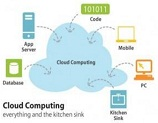
\includegraphics[scale=1]{saatu.jpg} \\
\textbf{Gambar 1.1} Ilustrasi Cloud Computing
\end{center}
\begin{center}
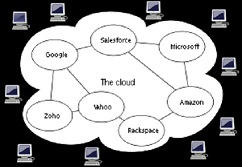
\includegraphics[scale=1]{sdua.jpg} \\
\textbf{Gambar 1.2} Diagram Konsep Cloud Computing
\end{center}
\tab yang menjadi pertanyaan, Apa bedanya dengan pemakaian komputer biasa selama ini? Pada pemakaian komputer biasa, diperlukan sistem operasi dan program aplikasi. Sistem operasi sangat menentukan program aplikasi. Kalau pemakai memilih sistem operasi MS Windows misalnya, maka aplikasinya pun harus berbasis Windows. Demikian juga kalau sistemnya berbasis DOS, Linux, Mac, dan sebagainya. Padahal memilih sistem operasi sendiri sering membuat user pusing, mau yang gratisan, atau yang berbayar? Program aplikasi harus dipasang di komputer sesudah sistem operasi terpasang. \\Untuk aplikasi berbasis DOS, relatif gampang, karena tidak perlu diinstal. Asal dikopi ke komputer, sudah siap dijalankan. Aplikasi ini sering disebut dengan stand alone software, karena tidak dapat dijalankan bersamaan dengan program lain. Keuntungannya, bila akan dijalankan di komputer lain, tinggal disalin saja, selesai. Tapi kalau sistemnya berbasis grafis dan multitasking (seperti MS Windows), program harus diinstal dulu. Kalau komputer lain diinginkan untuk menjalankan aplikasi tersebut, harus diisi dengan proses instal lagi, tidak bisa hanya dengan disalin seperti pada sistem DOS. Program seperti ini disebut dengan desktop application. Keunggulannya, dapat berjalan bersamaan dengan program lain. Kelemahannya, kalau ada program versi baru, harus beli lagi, instal lagi. Sebetulnya hal ini juga berlaku untuk program-program berbasis DOS.
\\Adapun struktur dari Cloud computing:
\begin{center}
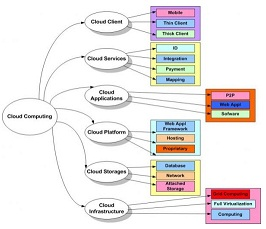
\includegraphics[scale=1]{stiga.jpg} \\
\textbf{Gambar 1.3} Struktur Cloud Computing
\end{center}
\section{Manfaat dan Tujuan Cloud Computing}
\tab Dengan adanya cloud computing akan mengubah paradigma perusahaan ataupun organisasi IT dalam memandang investasi teknologi komunikasi informasi. "Investasi untuk modal kapital berubah menjadi biaya operasional dengan besaran yang lebih efisien akibat adanya cloud computing,dan Ini membuat para pengguna (user) bebas berkreasi dan tidak perlu menyediakan infrastruktur (data center, processing power, storage, sampai ke aplikasi desktop) untuk dapat memiliki sebuah sistem, karena semuanya sudah disediakan secara virtual Disaat ini kebutuhan akan pemakaian , pemeliharaan dan keamanan sistem informasi semakin meningkat, mendorong perusahaan ataupun organisasi untuk meningkatkan dan mengamankan sistem mereka, namun Karena perusahaan ataupun organisasi tidak memiliki sumber daya yang besar untuk membeli sistem untuk keperluan mereka dan bahkan untuk memelihara sistem informasi mereka ,terlebih lagi untuk mengamankan sistem tersebut maka kemungkinan besar Cloud Computing akan menjadi pilihan pertama dan kemungkinan besar akan berkembang, khusunya di Indonesia. Bahkan dengan Cloud Computing, mereka (perusahaan / organisasi) hanya menyewa layanan atau jasa dari penyedia Cloud Computing.
\tab Seperti sudah dijelaskan sebelumnya dengan Cloud Computing ini dapat mengurangi investasi awal dari sebuah perusahaan atau organisasi yang membutuhkan pememakaian, pemeliharaan dan keamanan sistem informasi yanglebih baik. Dalam hal ini investasi yang besar bagi sebuah perusahaan atau organisasi akan berubah menjadi suatu sistem operasional yang mudah dikelola, bahkan penyedia jasa seperti Software as a Service (SaaS) yand ada di Cloud dapat menawarkan harga yang sangat rendah karena faktor ekonomi. Dengan Cloud Computing kita tidak perlu lagi dikuatirkan dengan adanya kompleksitas Teknologi saat ini. Perusahaan dan organisasi yang dalam usahanya menggunakan Teknologi Informasi tidak perlu takut dengan hal-hal yang dapat mengancam keamanan sistem informasi mereka dan bahkan dalam hal peng-updatetan suatu Teknologi atau aplikasi yang dipakai, karena semuanya itu bisa diserahkan kepada penyedia layanan di Cloud Computing. \\Cloud Computing jangan dijadikan sebagai "Core Business" bagi sebuah perusahaan tapi sebaliknya jadikan-lah Cloud Computing ini sebagai "Support Business", prinsip ini yang benar karena Cloud Computing sebagai penunjang suatu perusahaan dalam mengelola sistem informasi yang ada di perusahaan tersebut dengan maksud dan tujuan untuk kelangsungan bisnis dari perusahaan tersebut, karena Cloud Computing memberikan solusi bagi perusahaan untuk meringankan operasional perusahaan tersebut dalam hal pengolahan data. \\Manfaat Cloud Computing :
\begin{itemize}
\item Skalabilitas \\Mudah meningkatkan kapasitas, sebagai kebutuhan komputasi berubah, tanpa membeli peralatan tambahan.
\item Accessibility \\Akses data dan aplikasi melalui internet dari mana saja.
\item Mengurangi Biaya
\item Shift Beban \\Free staf TI internal dari pembaruan dan isu-isu konstan.
\end{itemize}
\tab Keprihatinan utama mengenai cloud computing adalah keamanan dan kehandalan. Banyak organisasi mengalami kesulitan mempercayai informasi mereka dengan vendor pihak ketiga, dan juga penyedia dipublikasikan padam telah meningkatkan keprihatinan mereka. Ketika mengevaluasi kebutuhan komputasi Anda, penting untuk mempertimbangkan baik manfaat dan risiko dari Cloud Computing. Sebagai contoh, data-kerugian yang mungkin baik itu dalam Cloud Computing dan sistem perusahaan tradisional, tetapi dalam banyak kasus vendor Cloud Computing akan memiliki lebih banyak sumber daya yang tersedia dengan cepat dan akurat memperbaiki kegagalan ini. Selain itu dengan teknologi Cloud Computing (komputasi awan) akan memberikan dampak lebih ekonomis dan sumber daya IT yang digunakan lebih efisien, saat aplikasi bisnis dioperasikan dalam suatu lingkungan. Jasa Cloud adalah bisnis yang paling cepat tumbuh dan berkembang pendekatannya untuk memberikan aplikasi dan layanan dari mana saja ke pelanggan apapun, pada perangkat apapun. Sebuah pergeseran yang terjadi dengan komputasi awan yang membentang di alam teknologi dan bisnis, sebuah pergeseran yang dramatis akan mengubah bisnis dan bagaimana menggunakan teknologi untuk memenuhi persyaratan. \\Dengan Cloud Kemampuan untuk menangani tugas-tugas penting, dapat dilakukan
lebih efisien oleh karena dilakukan oleh pihak ketiga, apakah mereka merupakan inti atau bukan inti dengan bisnis anda, adalah sebuah model bisnis yang umum dan merupakan layanan yang bisa menguntungkan anda.
Cloud computing membawa tujuh manfaat potensial, seperti :
\begin{enumerate}
\item Data yang disimpan terpusat.
\item Respon cepat.
\item Kehandalan kode uji.
\item Log (records tak terbetas).
\item Kinerja Perangkat Lunak dengan tingkat keamanan yang tinggi.
\item Konstruksi yang handal.
\item Menghemat Biaya uji keamanan yang mahal.
\end{enumerate}
\tab Selain itu cloud computing dapat memenuhi persyaratan skalabilitas untuk memenuhi permintaan pengguna dengan cepat, namun tidak mengharuskan pengguna untuk menjadi ahli pada bidang teknologi. Dengan teknologi ini kita dapat memfasilitasi workflow application yang berskala besar. Sehingga setiap user yang berorientasi pada penggunaan sistem yang berskala besar untuk keperluan organisasi atau perusahaan-nya, tidak perlu kuatir. Mengapa? teknologi ini (Cloud Computing) hadir untuk mengatasi itu. Sebagai contoh perusahaan yang memerlukan tempat penyimpanan yang besar untuk keperluan kerja perusahaan mereka, cloud dapat menyediakannya, tanpa harus perusahaan tersebut menyediakan server / storage yang besar untuk keperluan data mereka, yang sudah barangtentu memerlukan biaya yang besar. \\Selain itu manfaat dan tujuan dari cloud computing dalam rangka mendukung perangkat lunak yang di gunakan pada Cloud Computing adalah sebagai berikut :
\begin{enumerate}
\item Sistem penagihan yang terencana dan biaya untuk komputasi yang murah pada tingkat yang sangat mantap.
\item Memberikan performance database yang baik dan handal.
\item Memiliki jaminan keamanan yang tinggi yang didukung dengan dedicated server.
\item Memungkinkan pengguna dapat meminta penyimpanan dalam jumlah besar atau kecil dengan cepat serta menyediakan system penyimpanan yang terstruktur yang disebabkan karena ruang penyimpanan yang di atur secara teratur.
\item Mengefisienkan penggunaan aplikasi dan pengefisienan perangkat keras yang selama ini di pergunakan user (semuanya tersedia di Cloud Computing).
\item Menghemat / menekan penggunaan ruang yang berlebihan.
\item Mendukung program go green.
\end{enumerate}
\section{Sejarah Perkembangan Cloud Computing}
\tab Cloud (Awan) adalah suatu istilah yang dipinjam dari telepon. Sampai tahun 1990an, sirkuit data (termasuk yang membawa lalu lintas internet) yang berkabel keras diantara tujuan. Kemudian perusahaan telepon long-haul mulai menawarkan jasa Virtual Private Network (VPN) atau Jaringan Maya Privat untuk komunikasi data. Perusahaan telepon memungkinkan menyediakan layanan yang berdasarkan VPN dengan jaminan bandwidth sebagai sirkuit yang diperbaiki dengan biaya yang lebih murah karena mereka dapat mengganti lalu lintas untuk menyeimbangkan penggunaan yang mereka lihat cocok. Sehingga penggunaan jaringan mereka secara keseluruhan lebih efektif. Sebagai hasil dari penyusunan ini, memungkinkan untuk menentukan dengan cepat dan tepat jalan mana yang akan dilalui. Simbol cloud (Awan) digunakan untuk menunjukkan tanggung jawab sebuah provider (penyedia layanan), dan Cloud Computing (Komputerisasi awan) memperluasnya untuk melindungi server sebaik infrastruktur jaringannya. \\Hal yang mendasari konsep cloud computing berawal pada tahun 1960-an, saat John McCarthy, pakar komputasi MIT yang dikenal juga sebagai salah satu pionir intelejensi buatan, menyampaikan visi bahwa "suatu hari nanti komputasi akan menjadi infrastruktur publik--seperti listrik dan telpon". Namun baru di tahun 1995, Larry Ellison, pendiri Oracle, memunculkan ide "Network Computing" sebagai kampanye untuk menggugat dominasi Microsoft yang saat itu merajai desktop computing dengan Windows 95-nya. Larry Ellison menawarkan ide bahwa sebetulnya user tidak memerlukan berbagai software, mulai dari Sistem Operasi dan berbagai software lain, dijejalkan ke dalamPC desktop mereka. PC Desktop bisa digantikan oleh sebuah terminal yang langsung terhubung dengan sebuah server yang menyediakan environment yang berisi berbagai kebutuhan software yang siap diakses oleh pengguna. Ide "Network Computing" ini sempat menghangat dengan munculnya beberapa pabrikan seperti Sun Microsystem dan Novell Netware yang menawarkan Network Computing client sebagai pengganti desktop. \\Namun akhirnya, gaungNetwork Computingini lenyap dengan sendirinya, terutama disebabkan kualitas jaringan komputer yang saat itu masih belum memadai, sehingga akses NC (Network Computing) ini menjadi sangat lambat, sehingga orang-orang akhirnya kembali memilih kenyamananPC desktop, seiring dengan semakin murahnya harga PC. Merasakan ketidakpraktisan dengan program-program web-based, maka kini diciptakanlah suatu terobosan baru, yaitu Cloud Computing.
\tab Aplikasi yang ada di Cloud Computing tidak tergantung pada sistem operasi yang digunakan oleh pemakai (jadi boleh saja memakai Linux, Mac OS, MS Windows, bahkan sistem operasi PDA atau ponsel). Yang penting, user dapat mengakses Internet, menuju ke alamat atau situs tertentu, untuk menjalankan program yang dia perlukan.Contoh yang paling mudah dijumpai adalah aplikasi Google (di alamat www.google.com/apps) yang di antaranya terdiri atas organiser (pengelola data relasi, jadwal atau kalender, dan email) dan aplikasi bisnis (pengolah kata, pengolah angka, dan program presentasi). Aplikasi tersebut selain gratis, juga selalu diperbarui oleh pembuatnya. Pemakai tidak perlu membayar apapun, kecuali kalau membutuhkan fitur-fitur yang lebih bagus. \\Tonggak selanjutnya adalah kehadiran konsep ASP (Application Service Provider) di akhir era 90-an. Seiring dengan semakin meningkatnya kualitas jaringan komputer, memungkinkan akses aplikasi menjadi lebih cepat. Hal ini ditangkap sebagai peluang oleh sejumlah pemilik data center untuk menawarkan fasilitasnya sebagai tempat hosting aplikasi yang dapat diakses oleh pelanggan melalui jaringan komputer. Dengan demikian pelanggan tidak perlu investasi di perangkat data center. Hanya saja ASP ini masih bersifat "private", di mana layanan hanya dicustomisasi khusus untuk satu pelanggan tertentu, sementara aplikasi yang di sediakan waktu itu umumnya masih bersifat client-server. \\Kehadiran berbagai teknik baru dalam pengembangan perangkat lunak di awal abad 21, terutama di area pemrograman berbasis web disertai peningkatan kapasitas jaringan internet, telah menjadikan situs-situs internet bukan lagi berisi sekedar informasi statik. Tapi sudah mulai mengarah ke aplikasi bisnis yang lebihkompleks. Dan seperti sudah sedikit disinggung sebelumnya, popularitas Cloud Computing semakin menjulang saat di awal 2000-an, Marc Benioff ex VP di Oracle, meluncurkan layanan aplikasi CRM dalam bentuk Software as a Service, Salesforce.com, yang mendapatkan sambutan luar biasa di dunia Teknologi Informasi. Dengan misinya yang terkenal yaitu "The End of Software", Benioff bisa dikatakan berhasil mewujudkan visi bos-nya di Oracle, Larry Elisson, tentang Network Computing menjadi kenyataan satu dekade kemudian. Selanjutnya Cloud Computing bergulir seperti bola salju menyapu dunia teknologi informasi. Dimulai di tahun 2005, mulai muncul inisiatif yang didorong oleh nama-nama besar seperti Amazon.comyang meluncurkan Amazon EC2 (Elastic Compute Cloud), Google dengan Google App Engine-nya, tak ketinggalan raksasa biru IBM meluncurkan Blue Cloud Initiative dan lain sebagainya. 
\tab Semua inisiatif ini masih terus bergerak, dan bentuk Cloud Computing pun masih terus mencari bentuk terbaiknya, baik dari sisi praktis maupun dari sisi akademis. Bahkan dari sisi akademis, jurnal-jurnal yang membahas tentang hal ini baru bermunculan di tiga tahun belakangan. Akhirnya seperti yang kita saksikan sekarang, seluruh nama-nama besar terlibat dalam pertarungan menguasai "awan" ini. Bahkan pabrikan Dell, pernah mencoba mempatenkan istilah "Cloud Computing", namun ditolak oleh otoritas paten Amerika. Walaupun di luaran perebutan ?awan? ini begitu dasyat, tidak demikian dengan di tanah air Indonesia tercinta ini. Pemain yang benar-benar mencoba masuk di area ini masih sangat sedikit, bahkan jumlahnya bisa dibilang belum sebanyak jari sebelah tangan. Salah satu yang cukup serius bermain di area ini adalah PT Telkom, yang setidaknya saat ini sudah menawarkan dua layanan aplikasi berbasis Software as a Service. \\Salah satunya melalui anak usahanya, "Sigma Cipta Caraka", yang menawarkan layanan aplikasi core banking bagi bank kecil-menengah. Kemudian bekerjasama dengan IBM Indonesia dan mitra bisnisnya, PT Codephile, Telkom menawarkan layanan e-Office on Demand untuk kebutuhan kolaborasi/korespondensi di dalam suatu perusahaan atau organisasi. Sepinya sambutan dunia teknologi informasi dalam negeri terhadap Cloud Computing ini, mungkin disebabkan beberapa faktor, di antaranya:
\begin{enumerate}
\item Penetrasi infrastruktur internet yang bisa dibilang masih terbatas.
\item Tingkat kematangan pengguna internet yang masih menjadikan media internet utamanya sebagai media hiburan atau sosialisasi.
\item Tingginya investasi yang dibutuhkan menyediakan layanan cloud ini, karena harus merupakan kombinasi antara infrastruktur jaringan, hardware dan software sekaligus.
\end{enumerate}
\tab Namun demikian, sebagai negara dengan jumlah penduduk terbesar ke-5 di dunia, yang berarti juga pasar terbesar ke-5 di dunia, para pelaku teknologi informasi dalam negeri harus sesegera mungkin mempersiapkan diri dalam arti mulai mengembangkan layanan-layanan yang siap dicloud-kan. Sehingga saat gelombang besar Cloud Computing ini sampai di sini, tidak hanya pemain asing besar saja yang akan menangguk keuntungan. Tentu saja peran pemerintah sebagai fasilitator dan regulator sangat diperlukan di sini. Sampai saat ini paradigm atau pandangan tentang Cloud Computing ini masih berevolusi, dan masih menjadi subyek perdebatan yang melibatkan akademisi, vendor teknologi informasi, badan pemerintah, dan pihak-pihak terkait lainnya. Dan untuk memberikan satu common ground bagi publik, pemerintah Amerika melalui National Institut of Science and Technology (NIST) sebagai bagian dari Departemen Perdagangan Amerika, telah membuat beberapa rekomendasi standar tentang berbagai aspek dari Cloud Computing untuk dijadikan referensi. Beberapa contoh dari sejarah membuktikan bahwa telah berkembang konsep pembuatan kerangka kerja komputasi secara online tersebut - sebagai berikut :
\begin{itemize}
\item Sebuah portal internet yang memiliki berbagai fasilitas layanan umum mulai dari surat elektronik (e-mail), forum diskusi sampai dengan penyimpanan dokumen dengan media penyimpanan yang sangat luas (bahkan ada beberapa yang menyediakan dalam kapasitas tanpa batas/unlimited storage space) - sampai pada mekanisme berbagi dokumen, layananblogdsb. Kesemuanya disediakan dalam sebuah tempat.
\item Layanan Software as a Service atau SaaS dari berbagai vendor teknologi informasi terkemuka - mulai dari layanan pemindaian virus secara online hingga layanan pemindaianspam, dsb.
\item Layanan SpeedyWiki ini secara sederhana dapat dirujuk sebagai dasar-dasar Cloud computing dalam artian fasilitas SpeedyWiki ini dapat diakses dan dipergunakan secara bersamaan untuk berkolaborasi dalam menyusun dokumentasi yang sangat kompleks.
\item Aplikasi Point of Sale atau POS pada kasir pasar swalayan dengan metode Terminal Servicejuga dapat dikategorikan dasar-dasar Cloud Computing.
\end{itemize}
\section{Ragam Penerapan Cloud Computing}
\subsection{Fujitsu terapkan Cloud Computing}
\tab Komputasi awan (cloud computing) saat ini memang sedang marak dilakukan oleh
perusahaan-perusahaan IT, baik lokal maupun internasional. Kini vendor asal Jepang, Fujitsu, yang menerapkannya. perusahaan ini mengumumkan strategi global mereka untuk menerapkan cloud computing yang berlandaskan pada empat model pemakaian sumber daya komputasi, yaitu infrastruktur, aplikasi, aktivitas dan konten. Dalam strategi yang dikembangkan dari pengalaman Fujitsu selama bertahun-tahun, pelanggan bisa menerapkan sebagian atau seluruh model komputasi awan tanpa gangguan. \\Fujitsu telah menawarkan platform ini untuk model infrastruktur yang diperkuat dengan penerapan platform standar komputasi awan global secara luas. Fujitsu Indonesia telah mengembangkan teknologi komputasi awan dengan melihat perubahan dalam masyarakat dan bagaimana teknologi bisa membantu manusia melewati perubahan tersebut. "Inilah yang disebut sebagai sudut pandang human-centric. Di Jepang, Fujitsu berhasil menjalankan uji coba yang melibatkan pertanian dan kesehatan", ujar Achmad S. Sofwan selaku Chief Operation Officer Fujitsu Indonesia. Dimana Uji coba layanan ini sudah dilakukan pada bulan Mei 2010, dilanjutkan dengan komersialisasi pada Oktober 2010 di Jepang, Australia, Singapura, Amerika Serikat, Inggris dan Jerman. Platform komputasi awan global akan menjadi pelengkap platform awan lokal, dengan memenuhi kebutuhan infrastruktur Teknologi Informasi dan Komunikasi (TIK) yang terstandarisasi secara global. Dimana melalui cara ini, diharapkan pelanggan bisa mengadopsi layanan baik dari platform lokal maupun global secara fleksibel. \\Hasilnya, pelanggan bisa mengurangi biaya-biaya TIK, lebih tanggap terhadap kebutuhan bisnis dan bisa menyediakan layanan TIK tanpa mengorbankan keamanan dan tingkat ketersediaan. Pelanggan juga memperoleh manfaat dari keahlian Fujitsu dalam bidang telekomunikasi dan jaringan. Fujitsu sendiri melihat layanan cloud computing sebagi evolusi, bukan revolusi. Untuk itu, model pemakaian sumber daya komputasi di tingkat infrastruktur dan aplikasi adalah perpanjangan dari layanan konvensional yang selama ini ditawarkan Fujitsu. Namun di tingkat aktivitas dan konten, keduanya mencerminkan perubahan signifikan di industri TIK dalam hal menciptakan nilai dengan mengembangkan berbagai model bisnis dan layanan baru bagi para pembeli. \\Berbekal pengalaman selama beberapa dekade dalam menyediakan layanan bisnis, Fujitsu bisa memberikan dukungan kepada pelanggannya untuk berpindah dan bermigrasi ke model komputasi awan secara aman tanpa gangguan. Guna mewujudkan hal ini, perusahaan yang membuka cabang di Indonesia pada 1995 tersebut telah menjalin aliansi dengan sejumlah pihak yang terkait dengan komputasi awan. Mereka menjamin pelanggan tidak akan terjebak dalam sistem-sistem tertutup (proprietary). Berikut kutipan dari Corporate Senior Executive Vice President Fujitsu Richard Christou menyatakan bahwa "Fujitsu akan memberikan layanan komputasi awan terstandarisasi melalui platform cloud global yang digelar secara luas". "Kami akan memberikan pengumuman lanjutan untuk memenuhi fase-fase lain dari model komputasi awan, bersama dengan para mitra kunci di bulan-bulan mendatang. Fujitsu kini dalam posisi untuk bekerja bersama para pelanggan untuk mewujudkan manfaat komputasi awan".
\subsection{Penarapan Cloud Computing pada Google Docs}
\tab Google Docs adalah salah satu produk Google yang dapat mengolah (menyimpan,
membuat, meng-edit) program-program aplikasi perkantoran (seperti microsoft office jika diwindows) secaraonline, diantaranya program-programnya adalah pengolah kata (word processor), pengolah lembar kerja (spreadsheet) dan presentasi (presentation). Penggunakan fasilitas Google DOcs yang harus online/ terkoneksi lewat internet merupakan kelemahan dari program ini, namun aplikasi ini banyak mempunyai kelebihan, misalnya jika kita berpergian keluar kota atau bahkan keluar negeri untuk tujuan seminar atau apa saja kita tidak akan bingung ketinggalan dokumen jika semua sudah disimpan di Google Docs selain itu kita tidak akan kawatir dokumen akan hilang atau rusak seperti halnya jika kita menyimpan di harddisk yang sewaktu-waktu harddisk dapat rusak dan dokumen hilang. Berikut ini adalah hal-hal yang dapat kita lakukan dengan menggunakan Google Docs :
\begin{enumerate}
\item Dalam menggunakan dokumen, yang dapat dilakukan:
\begin{itemize}
\item Upload dokumen Word, OpenOffice, RTF, HTML, atau teks (atau membuat dokumen dari awal).
\item Menggunakan editor WYSIWYG yang sederhana untuk memformat dokumen, memeriksa ejaan, dll.
\item Sharing dengan orang lain (melalui alamat e-mail) untuk mengedit atau melihat dokumen dan spreadsheet.
\item Meng-edit dokumenonlinedengan siapa pun yang kita pilih.
\item Melihat riwayat revisi dokumen dan spreadsheet.
\item Mempublikasikan dokumen secara online ke dunia, sebagai halaman Web atau mengirimkan dokumen keblog.
\item Mendownload dokumen kedesktop sebagai Word, OpenOffice, RTF, PDF, HTML atau zip.
\item Email dokumen sebagai lampiran. \\Dalam menggunakan perangkat lunakspreadsheet, yangdapat dilakukan:
\end{itemize}
\begin{itemize}
\item Mengimpor dan mengekspor data berformat .xls, .csv, .txt dan .ods (dan mengekspor fungsionalitas untuk .pdf dan html).
\item Menikmati navigasi dan pengeditan intuitif, seperti dokumen atau spreadsheet tradisional.
\item Menggunakan format dan formula pengeditan.
\item Mengobrol dengan orang lain yang sedang mengedit.
\item Memasukkan spreadsheet, atau bagian dari spreadsheet, ke blog atau situs web kita. \\Dalam menggunakan perangkat lunak presentasi, yang dapat dilakukan:
\end{itemize}
\begin{itemize}
\item Mengimpor presentasi yang ada dalam jenis file ppt dan .pps.
\item Mengekspor presentasi kita menggunakan fitur Simpan sebagai Zip dari menu File.
\item Mengedit presentasi kita menggunakan editor WYSIWYG yang sederhana.
\item Menyisipkan gambar, dan memformat slide kita agar sesuai dengan keinginankita.
\item Berbagi-pakai dan mengedit presentasi bersama teman dan rekan kerja.
\item Mengizinkan melihat presentasi pada waktu-nyata, online, dari lokasi jauh yang terpisah.
\item Mempublikasikan presentasi kita di web, dan dapat di akses oleh orang lain. \\Untuk besarnya dokumen yang dapat kita kerjakan dalam Google Docs adalah :
\end{itemize}
\end{enumerate}
\begin{enumerate}
\item Dokumen \\
\begin{itemize}
\item Setiap dokumen dapat mencapai sebesar 500K, ditambah 2MB per gambar yang dimasukkan.
\item Dapat meng-upload dokumen dengan format file berikut : \\
\begin{enumerate}
\item HTML
\item Teks biasa (.txt)
\item Microsoft Word(.doc)
\item .rtf
\item Open Office (.odt)
\item Setiap pengguna memiliki batas kombinasi 5000 dokumen dan presentasi serta 5000 gambar.
\end{enumerate}
\end{itemize}
\item Spreadsheet \\
\begin{itemize}
\item Setiapspreadsheet dapat mencapai hingga 10,000 baris, atau hingga 256 kolom, atau hingga 100,000 sel, atau hingga 40 sheet batas mana saja yang tercapai lebih dulu.
\item Setiap pengguna memiliki batas hingga 200 spreadsheet.
\item Batas untuk spreadsheet terbuka pada saat bersamaan adalah 11.
\item Dapat mengimpor spreadsheet hingga mencapai 1 MB dalam format xls, csv, atau ods, txt, tsv, tsb.
\end{itemize}
\item Presentasi \\
\begin{itemize}
\item Setiap presentasi dapat mencapai sebesar 500K, ditambah 2MB per gambar yang dimasukkan.
\item Kita dapat meng-uploadpresentasi dalam format .ppt maupun .pps.
\item Setiap pengguna memiliki batas kombinasi 5000 dokumen dan presentasi serta 5000 gambar
\end{itemize}
\end{enumerate}
\subsection{Penerapan Cloud Computing pada Salesforce.com}
\tab Salesforce.com adalah aplikasi Customer Relationship Management (CRM) berbasis
software as services, dimana kita bisa mengakses aplikasi bisnis: kontak, produk, sales tracking, dashboard, dll. Penerapan Cloud Computing pada Amazon Web Services (AWS) Amazon menawarkan berbagai macam service yang sangat mirip dengan serviceservice yang terdapat pada suatu jaringan konvensional. Membangun jaringan virtual dengan Amazon Web Services sangat mudah dilakukan, namun ada sedikit kesulitan menentukan standar dalam infrastruktur Amzon Web Services, yang disebabkan oleh tidak ada batasan dari penggunaan setiap service yang ada pada Amazon Web Servicies.
\subsection{Penerapan Cloud Computing pada Microsoft Windows Azure (MWA)}
\tab Pada MWA user dimungkinkan untuk mengembangkan aplikasi-aplikasi dengan basis
NET. Dimana user mengembangkan jaringan sesuai dengan kebutuhan, namun MWA menetapkan standar-standar yang tidak bisa dilanggar. Dapat dikatakan atau disimpulkan bahwa MWA merupakan framework-framework aplikasi lengkap yang diimplementasikan dalam jaringan virtual yang memiliki basis yang sama dengan jaringan konvensional.
\subsection{Penerapan Cloud Computing pada Biznet}
\tab Biznet Cloud Computing adalah platform komputer generasi masa depan yang dapat
memberikan keuntungan untuk perusahaan, dimana keuntungannya tetap fokus pada bisnis, tanpa harus memikirkan cara untuk setup, operasi dan menjaga platformkomputer yang berkembang. Platform Biznet Cloud Computing menyediakan pilihan beberapa prosesor, ukuran memory, storage (hard disk) dan berbagai jenis Operating System. Platform ini juga secara otomatis melakukan load balancing sehingga dapat mengirim aplikasi secara maksimal. \\Biznet Cloud Computing menyediakan kemampuan proses komputerisasi dengan standar -standar sebagai berikut :
\begin{itemize}
\item Pilih platform server dan ukuran sesuai kebutuhan
\item Dapat men-setup beberapa server dalam hitungan menit
\item Teknologi virtualisasi berbasis VMware ESXi
\item Akses online melalui control panel danopen API
\item Administration dengan root access
\item Kapasitas Backbone Global Internet Tier-1 secara redundant dengan beberapa Gbps
\item Minimum kontrak 6 bulan
\end{itemize}
\begin{table}
    \begin{tabular}{|c|c|c|}
        \hline
        Layanan                                            & Biaya Bulanan ( Rp ) & Biaya Setup ( Rp ) \\ \hline
        Cloud Server 1 Core, 1 GB RAM, 100 GB SAN Storage  & 2,250,000            & 2,000,000          \\ \hline
        Cloud Server 2 Core, 2 GB RAM, 100 GB SAN Storage  & 3,000,000            & 2,000,000          \\ \hline
        Cloud Server 4 Core, 4 GB RAM, 100 GB SAN Storage  & 4,000,000            & 2,000,000          \\ \hline
        Cloud Server 8 Core, 8 GB RAM, 100 GB SAN Storage  & 5,750,000            & 2,000,000          \\ \hline
        Cloud Server 8 Core, 16 GB RAM, 100 GB SAN Storage & 9,000,000            & 2,000,000          \\ \hline
        Cloud Server 8 Core, 32 GB RAM, 100 GB SAN Storage & 14,500,000           & 2,000,000          \\
        \hline
    \end{tabular}
\end{table}
\tab Seluruh paket Cloud Server termasuk bandwidth inbound \& outbound sebesar 500 GB. Setelah alokasi bulanan telah terpakai, maka ada biaya tambahan sebesar Rp. 2,000/GB untuk tambahan bandwidth yang terpakai. Pada Biznet, pengguna Cloud Computing hanya membayar layanan yang mereka pakai, dimana layanan yang dipakai disesuaikan dengan kebutuhan dari setiap pengguna (user). Sehingga proses pembayaran dilakukan juga sesuai dengan layanan yang mereka pakai (sesuai kebutuhan). Satu virtual Data Center dari layanan Cloud Computing dapat dibagi menjadi beberapa mesin virtual. (kutipan dari Presiden Director Biznet Networks, Adi Kusuma). Cloud Computing adalah teknologi penyimpanan data secara virtual, yang memungkinkan user (pengguna) dapat menyimpan data secara konvensional. \\Melalui Biznet, Cloud Computing yang difokuskan kepada para pengusaha UKM, dimana pengusaha UKM (dalam hal ini sebagai pemilik data) dapat fokus ke bisnis mereka tanpa harus memikirkan biaya yang harus dikeluarkan untuk "membangun" penyimpanan data, karena semua layanan ini dapat disewa dengan mudah, cepat dan yang pasti harga terjangkau. Selain menghemat biaya, Cloud Computing juga mendukung gerakan Green Computing. Ini disebabkan karena layanan Cloud Computing menggunakan server blades yang sangat efisien dalam penggunaan ruang data center dari konsumsi listrik, sehingga dapat mengurangi pemakain listrik yang berlebihan serta polusi lingkungan akibat pembangunan data center yang tidak efisien. Berikut ada beberapa paket yang ditawarkan, antara lain : Cloud Server dengan biaya bulanan Rp. 2,5 juta/bulan, Cloud Hosting Rp. 7 juta/bulan, dan Cloud Storage Rp. 3 juta/bulan.
\section{Riset Cloud Computing}
\tab sumber dari kompas.comdantechno.okezone.com \\
\tab PT Telekomunikasi Indonesia Tbk (Telkom) memperkirakan nilai pasar cloud computing di Indonesia mencapai Rp 2,1 triliun tahun depan. Direktur Whole Sales and Enterprise Telkom Arief Yahya menjelaskan, dari tiga jenis layanan yang bisa diberikan teknologi cloud computing yaitu Software as a Service (SaaS), Platform as a Service (PaaS) dan Infrastructure as a Service (IaaS), maka layanan SaaS paling banyak digunakan. "Dari nilai pasar Rp 2,1 triliun, SaaS menyumbang 40 persen. Kami sendiri akan mengupayakan untuk bisa menguasai pasar sampai 70 persen," kata Arief, Senin (18/10/2010). Arief menambahkan, pasar yang paling banyak menyerap teknologi cloud computing berasal dari instansi pemerintah. Misalnya National Single Windows (NWS), yang berhasil membuat semua pelaku usaha berlomba mendukung program tersebut. \\Hal ini didukung pula oleh belanja IT pemerintah daerah dan pemerintah pusat yang lumayan besar, khususnya untuk pendidikan dan kesehatan. "Di sektor pendidikan saja, ada alokasi Rp 200 triliun, dimana 20 persen untuk belanjaIT". Untuk itu, pemerintah daerah diharapkan tidak segan untuk memanfaatkan cloud computing karena bisa menekan biaya investasi dan menciptakan efisiensi. "Supaya Cloud Computing bisa berkembang, pemerintah harus menerbitkan aturan yang bisa mendorong kerjasama. Mulai dari pemasaran hingga kepemilikan bersama. Di bisnis software saja banyak sekali pemain asingnya. Padahal Cloud Computing modalnya kreativitas. Direktur Utama Teknologi Riset Global Investama (TRG Investama) Gatot Tetuko mengakui, perusahaannya mulai tertarik untuk mencicipi rezeki di bisnis layanan Cloud Computing. "Setelah aktif di penyedian menara dan perangkat Wimax, mereka akan melebarkan sayap ke Cloud Computing karena peluangnya bagus ke depan. TRG Investama adalah pemilik sebagian saham Indonesian Tower dan TRG.
\tab Di bisnis Cloud Computing, TRG Investama akan mengeluarkan merek dagang "Indonesian Cloud". Langkah pertama yang disiapkan oleh perusahaan ini untuk menggarap bisnis cloud computing adalah menggandeng Institut Teknologi Bandung untuk melakukan riset tentang konten-konten spesifik yang terkait dengan Cloud Computing. Dimana TRG Investama menanam Rp 10 miliar untuk melakukan riset hingga jangka waktu tiga tahun mendatang. Cloud computing sama dengan konsep berbagi infrastruktur. Seperti diketahui, selain berpengalaman di bisnis penyediaan menara, Indonesian Tower juga dikenal sebagai penyedia perangkat WiMax. "Ini adalah peluang masa depan yang harus dioptimalkan anak bangsa", tegas Gatot. Menurut dia (Gatot), TRG Investama memiliki keunggulan independen sebagai perusahaan Cloud Computing. \\Pasalnya, posisi independen membuat TRG Investama bebas untuk bekerjasama dengan semua lapisan. Dimana yang menjadi sasaran utama TRG Investama adalah pasar pemerintah dan Usaha Kecil Menegah (UKM). Perlu diketahui,TRG Investama sendiri adalah perusahaan investasi yang memfokuskan diri pada inovasi dan pengembangan teknologi di Indonesia. Dengan dorongan untuk mengembangkan teknologi baru, didukung dengan advance engineering dan manajemen yang berkualitas, TRG Investama bertujuan untuk menciptakan industrial powerhouse di Indonesia melalui anak perusahaannya. Sebelumnya, lembaga riset Gartner memperkirakan dalam waktu dua tahun mendatang sebanyak 80 persen dari perusahaan besar di dunia akan menggunakan Cloud Computing untuk meningkatkan daya saingnya. International Data Corporation memperkirakan tahun lalu pendapatan dari public cloud mencapai 16 miliar dollar AS dan diperkirakan pada 2014 akan mencapai 55,5 miliar dollar AS.
\subsection{Pergerakan Komputasi Awan(Cloud Computing)Semakin Cepat}
\tab sumber dari detik.com \\Sebanyak 83 persen perusahaan berskala besar di Asia Pasifik menilai komputasi awan sebagai teknologi yang relevan bagi bisnis mereka. Persentase ini meningkat lebih dari dua kali lipat dalam 18 bulan terakhir. Demikian hasil survei Springboard Research yang disponsori penyedia solusi virtualisasi VMware. Survei terhadap 6.593 responden pada Bulan September, menunjukkan pergerakan komputasi awan di tujuh pasar Asia Pasifik meningkat pesat selama 18 bulan terakhir ini,khususnya di kalangan perusahaan berukuran besar. Kini, sebanyak 59 persen dari firma regional telah menggunakan atau berencana memakai inisiatif awan (cloud), dibandingkan 45 persen enam bulan lalu dan 22 persen pada 2009. \\Organisasi di Jepang dan Australia memimpin adopsi Awan(cloud), masing-masing dengan 36 persen dan 31 persen telah menjalankan inisiatif yang berkaitan dengan awan(cloud). India dan China adalah yang terdepan dalam hal rencana adopsi, masing-masing 43 persen dan 39 persen tengah berencana menerapkan komputasi Awan(Cloud Computing). Untuk pasar ASEAN, perusahaan di Singapura memimpin dengan 23 persen, disusul Malaysia dan Thailand dengan masing-masing 21 persen. Namun untuk perencanaan awan(cloud), Malaysia dan Thailand adalah yang terdepan masing-masing 29 persen dibandingkan Singapura. Perusahaan-perusahaan yang ahli IT seperti telekomunikasi dan teknologi memimpin baik dalam hal adopsi awan maupun rencana adopsi awan. Perusahaan-perusahaan berukuran besar - terutama yang mempekerjakan lebih dari 10.000 karyawan, memimpin adopsi Awan (39 persen) dibandingkan organisasi yang lebih kecil dengan 100-999 karyawan (20 persen).
\subsection{Teknologi Informasi Berbasis Layanan}
\tab Sebagian besar perusahaan di Jepang (86), Singapura (84) dan Thailand (74)
mengasosiasikan komputasi awan(Cloud Computing) dengan IT-as-a-Service (ItaaS) atau TI sebagai layanan. Di Australia (80), Malaysia (78) dan India (75) mengasosiasikan awan sebagai application-on-demand. Di China, sebanyak 80 responden melihat Awan(cloud) sebagai cara untuk menyediakan storage danjaringan sesuai kebutuhan (on-demand). "Bagi sebagian besar responden survei di Asia Pasifik, TI sebagai layanan adalah tema terbesar hari ini. Perusahaan-perusahaan seperti itu mencari vendor dan konsultan yang mampu membantu mereka menikmati TI berbasis layanan, terutama di area infrastruktur dan manajemen Awan", kata Michael Barnes, VP of Software \& Asia Pacific Research, Springboard Research dalam keterangannya yang dikutip detikINET, Selasa (9/11/2010). Lebih dari separuh organisasi (60) ingin mengadopsi awan(cloud) untuk mencapai skalabilitas sesuai permintaan sehingga bisa lebih cepat memenuhi kebutuhan bisnis, mengurangi biaya infrastruktur peranti keras dan pengadaan server dan sumber daya yang lebih sederhana. Penghematan biaya adalah daya tarik utama dalam mengadopsi komputasi Awan(Cloud Computing), bagi 57 perusahaan di Asia Pasifik. Hanya 37, umumnya perusahaan berukuran besar dengan lebih dari 10.000 karyawan, mengadopsi atau berencana mengadopsi Awan sebagai investasi strategis dalam jangkapanjang.
\subsection{Cloud Computing: Sensasi Masa Depan Dunia IT}
\tab Cloud Computing diperkirakan akan mengubah TI di perusahaan besar karena memungkinkan enterprise dari berbagai ukuran untuk memanfaatkan skala ekonomi dan mendapat keuntungan dari hanya membayar sumber daya yang digunakan saja. Sesungguhnya, banyak aspek komputansi yang sudah (atau akan) tersedia dalam bentuk layanan cloud: Infrastructure as a Service (IAAS) seperti Amazon Services, Microsoft Windows Azure, VMWare vCloud serta Eucalyptus dan Cloudera yang open-source menyediakan komputansi, jaringan serta kapasitas penyimpanan yang elastic. Software as a Service (SAAS) merujuk pada aplikasi online, termasuk software produktivitas, database dan proses bisnis. \\Contoh SAAS termasuk Microsoft Business Productivity Online Suite (BPOS), Google Docs dan Gmail, Salesforce CRM dan Oracle CRM on Demand. Sedangkan, Platform as a Service (PASS), memungkinkan pengembangan aplikasi (contoh, Google Apps dan Windows Azure), Desktop as a Service (DAAS), dan bahkan apa yang disebut sebagai XAAS atauEAAS, yaitu "Everything as a Service". Dengan cloud computing, heterogenitas telah menjadi sebuah karakteristik utama dari komputansi. Sumber daya di awan bisa jadi proprietary atau open-source atau gabungan dari keduanya. Contoh yang menarik bisa dilihat dari profil penawaran dari satu perusahaan berikut ini: Citrix menawarkan aplikasi proprietary seperti GoToMeetings untuk komunikasi desktop dan software konferensi, serta Desktops To Go untuk aplikasi remote desktop. Bersama itu, mereka juga menawarkan produk Open-source seperti server Xen dan XenDesktop, sebuah virtual desktop.
\tab Proyek open-source Xen, yang berada di Citrix, telah melahirkan insiatif bernama Xen Cloud Platform, didukung oleh Citrix, Hewlett-Packard, Intel, Oracle dan Novell. Dengan aplikasinya di Apple iPad, Corix Receiver, Citrix bisa menghadirkan desktop Windows pada iPad, sehingga fungsi desktop dan aplikasi Windows bisa diakses sepenuhnya. Ada tujuh produk Cloud baru, tergabung dalam Citrix Cloud Solutions, yang bersifat open-source dan bisa diperluas sesuai kehendak pengguna. Citrix menyebut Cloud Solutions ini sebagai framework yang memungkinkan interoperabilitas dengan software lain, termasuk virtualisasi pihak ketiga seperti VMWare yang merupakan pesaingnya. Bukan hanya bersifat heterogen karena mencampurkan solusi proprietary dan opensource-- cloud computing juga bersifat global. Sebagai contoh, Windows Azure tersedia di 41 negara. \\Di cloud, pengguna bisa saja mengakses aplikasi yang di-hosting di Hong Kong dari kantornya di Korea Selatan. Datanya, bisa jadi disimpan di server yang ada di Polandia routingnya melalui Amerika Serikat. Dari sudut pandang pengembang piranti lunak, sifat yang global dari cloud ini tak hanya ditentukan oleh perilaku jejaringnya, tapi juga struktur bisnis itu sendiri. Peneliti yang bekerja untuk perusahaan multinasional asal AS di Russia mungkin berkolaborasi dengan tim di Singapura. Produk akhirnya bisa jadi dirancang di AS dan Taiwan, dibuat di India, Malaysia, dan Filipina untuk dijual di Amerika Selatan. Peluang ekonomi ada bagi negara yang memiliki kebijakan publik dan hukum yang netral secara teknologi dan kompatibel. Contohnya, pemerintah Singapura yang sejak lama menyadari bahwa teknologi mendorong pertumbuhan ekonomi negara itu. Di 2008, pemerintahannya bekerjasama dengan Hewlett Packard, Intel dan Yahoo, serta lembaga penelitian di Russia, Jerman dan AS untuk membuat test bed open-source yang mendukung penelitian layanan cloud pada skala global. HP juga membuka Cloud Labs di Singapura. Di saat yang sama, pemerintahannya memberi subsidi pada proyek yang bisa memberikan Cloud Computing pada eGovernment dan Usaha Kecil Menengah. Singapura adalah pemimpin dalam melihat Cloud Computing sebagai alat menumbuhkan ekonomi IT-nya serta menjaga perannya di pasar global. Memang masih di tahap awal, tapi jelas bahwa ini akan mengubah komputansi di enterprise, memenuhi kebutuhan pengguna dengan kelenturan yang belum pernah dilihat sebelumnya. \\Dengan makin tumbuhnya Cloud Computing, maka semakin penting bagi pembuat kebijakan untuk menjamin bahwa kebijakan domestiknya tidak berpihak pada teknologi tertentu. Bukan hanya untuk memenuhi kebutuhan perdagangan global, hukum internasional dan kepentingan pertumbuhan ekonomi, hal ini juga memungkinkan perusahaan domestik untuk meraup keuntungan besar dari peluang yang dihasilkan cloud computing.
\subsection{Membangun Infrastruktur Cloud Computing Masa Depan}
\tab sumber : CHIP.co.id \\Cloud Computing membawa perubahan mendasar pada cara orang dan berbisnis menggunakan internet serta perangkat komputasi. Tercatat 175 exabyte data melintasi internet pada tahun 2010, setara dengan 43.750 juta DVD. Dengan kondisi seperti ini, evolusi Cloud Computingyang mengandung arti lebih banyak pengguna, lebih banyak perangkat, konten lebih kompleks dan harapan yang lebih besar di mana saja, kapan saja untuk mengakses data. Cloud Computing menjadi sebuah kenyataan di Asia Pasifik dan industri telah mulai berpikir tentang bagaimana hal ini akan menguntungkan dan memajukan bisnisdi masa akan datang. Jason Fedder, General Manager, Asia Pasific \& Cina, Data Center Products Group,
Intel, mengundang CHIP.co.id bergabung dalam telekonferensi dengan wartawan dari berbagai negara di Asia Pasific dan Cina dalam sebuah diskusi tentang masa depan Cloud Computing. Pada telekonferensi kali ini dibicarakan teknologi yang dibutuhkan untuk mendukung Cloud Computing dan kemitraan di masa depan. Intel membagikan visi pada CHIP.co.id tentang Cloud Computing di Tahun 2015, dan menjelaskan beberapa gagasan dan istilah, tentang Cloud yaitu Federated, Automated, Client Aware.
\begin{enumerate}
\item Federated berarti sejumlah data yang ada pada berbagai perangkat dapat dipertukarkan secara aman melalui Cloud, baik lintas publik maupun private.
\item Automated berarti Pertukaran data tersebut juga dapat berjalan sendiri secara otomatis sehingga di masa depan, berbagai pihak dapat lebih fokus pada inovasi dan berkurang dari sisi manajemen data.
\item Client Aware berarti, layanan bisa dioptimasi, ditingkatkan sesuai dasar kemampuan perangkat yang ada.
\end{enumerate}
\tab Selain tiga hal ini Jason Fedder juga membahas Open Data Center Alliance di mana lebih dari 70 bisnis global disatukan oleh Intel untuk membuat panduan untuk interoperabilitas, fleksibilitas dan standar industri untuk Cloud Computing. Open Data Center Alliance ini telah diluncurkan sejak 27 Oktober 2010. Intel juga membentuk Intel ® Cloud Builders, sebuah kemitraan 20 hardware terkemuka di dunia dan pembuat perangkat lunak yang akan menjadi referensi serta mengikat sumber daya untuk mendorong inovasi dan membuat teknologi Cloud Computingmudah untuk disebarkan, digunakan dan berbagi pengetahuan. Yang menjadi pertanyaan bagaimana dengan perkembangan Teknologi Cloud Computing untuk masa yang akan datang di Indonesia? "Cloud computing tidak bisa dihindari, dengan menggunakan layanan tersebut para pelaku industri akan lebih meningkatkan efisiensi perusahaannya, terutama untuk kelas UKM (usaha kecil menengah)", jelas Philip Sargeant, Research VP Gartner kepada sejumlah wartawan, seperti yangdilansir oleh laman detikcom. \\Menurut data Gartner, di tahun 2010 ini diperkirakan nilai bisnis dari pemanfaatan teknologi internet untuk menyediakan sumber komputer itu sendiri secara global mencapai USD 80 miliar dengan tingkat pertumbuhannya setiap tahun sebesar 25 persen dalam jangka waktu lima tahun mendatang. Jadi, bisnis ini akan menjadi bisnis yang akan semakin ramai seiring dengan murahnya harga bandwidth. Semua tergantung kebutuhan, jika data bersifat tidak confidential saat ini pun bisa dimulai. Sebaliknya jika memerlukan sistem keamanan yang baik, maka akan bisa dimulai beberapa tahun kedepan, tergantung dari layanan yang dibutuhkan.
\let\cleardoublepage\clearpage
\chapter{Pengembangan Element Cloud Computing}
\date{}
\section{Topologi Jaringan \textit{Cloud Computing}}
Berbicara tentang sistem \textit{Cloud computing}, akan sangat membantu bila kita membaginya menjadi dua kelompok, yakni : front-end dan back-end. Keduanya terhubung melalui sebuah jaringan (Internet). Front-end terletak pada sisi pengguna atau client. Sementara back-end adalah bagian "awan" dalam sistem ini (dalam diagram jaringan internet kerap digambarkan sebagai awan).\\
\tab Front-end mencakup komputer (atau jaringan komputer) client, dan aplikasi yang diperlukan untuk mengakses sistem \textit{Cloud computing}. Tidak semua sistem \textit{Cloud computing} memilikin interface yang sama. Untuk mengakses layanan Web 2.0 seperti email berbasis web hanya dibutuhkan web browser biasa, seperti Firefox, Internet Explorer, atau  Opera.
Namun, adapula sistem\textit{Cloud computing} yang memiliki aplikasi sendiri \textit{(proprietary)} yang harus diinstall di komputer client. Sementara itu, pada sisi backend dari sistem \textit{Cloud computing} terdapat beragam komputer, server, dan sistempenyimpanan data, yang kesemuanya menciptakan "awan" bagi layanan komputasi.
\\
\tab Secara teori, sebuah sistem\textit{Cloud computing} mencakup semua programkomputer yang dapat Anda bayangkan, dari data processing hingga video game. Biasanya, setiap aplikasi dijalankan dan memiliki server sendiri (dedicated server). Sebuah server pusat mengatur jalannya sistem, seperti memonitor lalu lintas, dan permintaan client untuk memastikan semuanya berjalan dengan baik.\\
Bila sebuah perusahaan \textit{Cloud Computing} memiliki banyak client, maka kebutuhan akan ruang penyimpanan data (storage space) pun akan membengkak. Sistem \textit{Cloud Computing} paling tidak membutuhkan ruang penyimpanan data dua kali lebih besar daripada kebutuhan riil untuk membuat salinan (copy) semua data client. Hal ini dimaksudkan untuk mencegah kehilangan data bila terjadi gangguan pada media penyimpanan utama.\\

\begin{center}
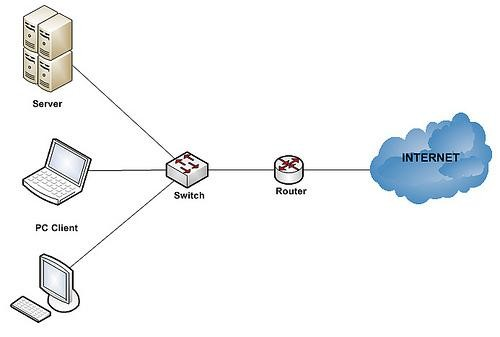
\includegraphics[scale=1]{gambar21.jpg} \\
\textbf{Gambar  2.1} gambaran umum topologi \textit{Cloud computing}
\end{center}
\textbf{Distribusi beban vertikal untuk Komputasi Awan melalui Pilihan Implementasi  Multiple.}
\\\\
\textit{Cloud Computing} menyediakan perangkat lunak sebagai layanan "cadangan" untuk pengguna terakhir, tapi infrastruktur yang mendasari harus cukup terukur dan kuat.dan harus fokus pada sistem \textit{Cloud} perusahaan skala besar dan meneliti  bagaimana  perusahaan dapat menggunakan service-oriented architecture (SOA) untuk menyediakan antarmuka yang efisien untuk proses bisnis.\\
\tab Untuk meningkatkan proses bisnis, masing-masing tingkatan SOA biasanya menyebarkan beberapa server untuk muatan distribusi dan toleransi kesalahan. Salah satu keterbatasan dari pendekatan ini adalah beban yang tidak dapat didistribusikan lebih lanjut saat semua server pada tingkatan /jajaran yang sama dimuat.\\
\textit{Cloud computing} terlihat untuk perhitungan dan penyimpanan data menjauh dari end user dan ke server yang berlokasi di pusat data, dengan demikian mengurangi beban pengguna dari penyedian aplikasi dan manajemen. \\
\tab Dalam sistem awan enterprise, arsitektur berorientasi layanan  (SOA)  dapat digunakan untuk menyediakan antarmuka yang mendasari proses bisnis, yang ditawarkan melalui awan(\textit{cloud}). SOA dapat bertindak sebagai sebuah front-end terprogramke berbagai komponen layanan yang dibedakan           sebagai individu dan pendukung server. Permintaan yang masuk ke layanan yang disediakan oleh gabungan SOA harus diteruskan ke komponen yang benar dan server masing-masing, dan seperti routing harus  terukur untuk mendukung sejumlah besar  permintaan.\\
Dalam rangka untuk meningkatkan proses bisnis, setiap tingkatan dalam sistem biasanya menyebarkan beberapa server untuk mendistribusikan beban dan toleransi kesalahan. seperti distribusi beban di beberapa server dalam tingkat yang sama dapat dilihat sebagai distribusi beban horisontal, tampak seperti gambar berikut :\\
\begin{center}
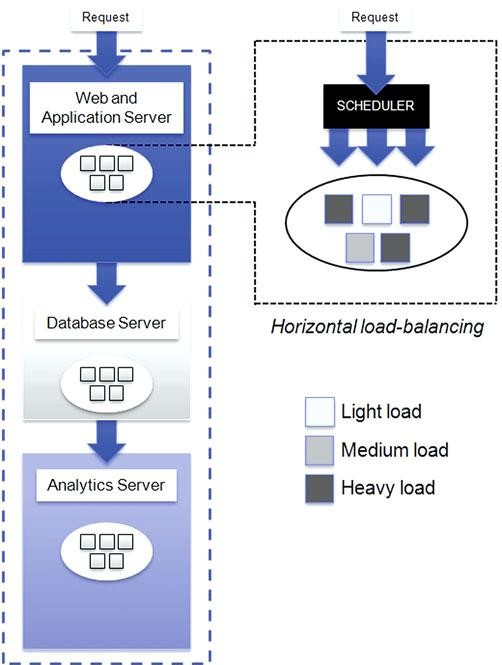
\includegraphics[scale=1]{gambar22.jpg} \\
\textbf{Gambar 2.2} Horizontal distribusi beban: beban didistribusikan di dalamserver, dalamtingkat yang sama.
\end{center}
Salah satu batasan dari distribusi beban horisontal adalah bahwa beban tidak dapat didistribusikan lebih lanjut ketika semua server dalam tingkatan tertentu mengambil hasil dari kesalahan konfigurasi infrastruktur. dimana terlalu banyak server yang dikerahkan pada satu tingkat sementara dilain pihak ada sedikit server yang dikerahkan di lain tingkatan.\\
\tab Sebuah pengamatan penting adalah bahwa dalam sistem kompleks SOA multi-tier, proses bisnis tunggal sebenarnya bisa dilaksanakan oleh beberapa jalur yang berbeda melalui tingkat perhitungan dalamrangka memberikan ketahanan dan skalabilitas.\\
Sebuah layanan komposit dapat direpresentasikan sebagai tingkatan pemanggilan beberapa komponen dalam sebuah infrastruktur TI berbasis SOA. Dalam sistem seperti itu, kami membedakan distribusi beban horisontal, dimana beban dapat tersebar di  beberapa  server untuk satu komponen layanan, dari distribusi beban vertical, dimana beban dapat tersebar di beberapa implementasi dari layanan yang diberikan. Gambar berikut menggambarkan istilah- istilah di atas.\\\\
\begin{center}
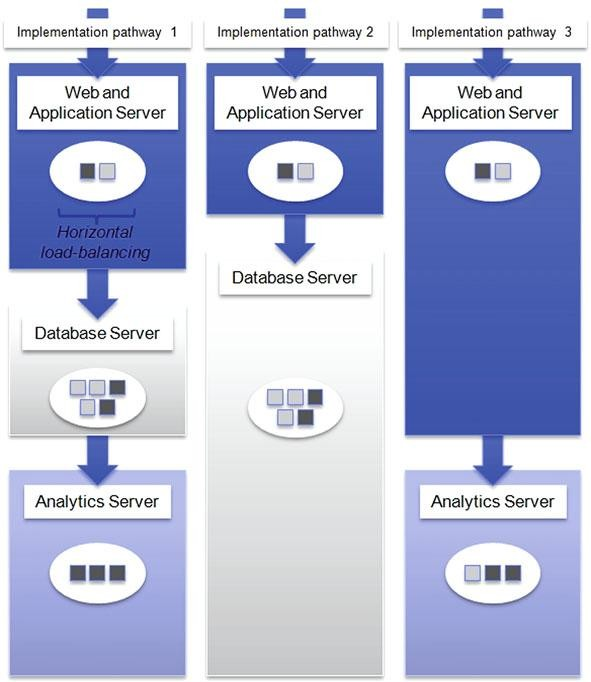
\includegraphics[scale=1]{gambar23.jpg} \\
\textbf{Gambar  2.3} Distribusi beban vertical.
\end{center}
Berikut tugas analitik komposit online dapat direpresentasikan sebagai panggilan  untuk Web  dan Aplikasi Server (WAS) untuk melakukan pra-pemrosesan tertentu, diikuti dengan sebuah panggilan dari WAS ke server database (DB) untuk mengambil  data yang dibutuhkan,  setelah itu WAS meneruskan data yang ditetapkan ke server analitik khusus untuk tugas-tugas komputasi data mining yang mahal.\\
\tab Tugas komposit memiliki beberapa implementasi di pusat data modern IT. Implementasi alternatif dapat memanggil prosedur yang tersimpan pada database untuk menjalankan data mining dan bukan memiliki server analitik khusus untuk melakukan tugas ini. Implementasi alternatif menyediakan distribusi     beban vertikal dengan memungkinkan penjadwalan pekerjaan untuk memilih\ implementasi WAS-dan-DB saat analitik server tidak tersedia.\\
\textit{Reusability} adalah salah satu tujuan utama dari pendekatan SOA. Sehubungan dengan reusability yang tinggi dari komponen aplikasi, adalah mungkin untuk menentukan alur kerja yang kompleks dengan beberapa cara. Namun sulit untuk menilai, mana yang merupakan penerapan yang terbaik.\\
Pada bagian ini diberikan gambaran sistem arsitektur dan contoh komputasi awan yang disederhanakan(seperti  gambar berikut).\\
\begin{center}
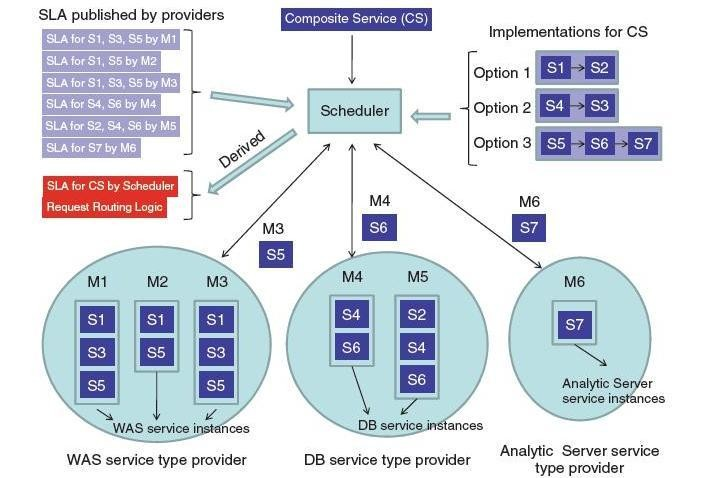
\includegraphics[scale=1]{gambar24.jpg} \\
\textbf{Gambar  2.4} Request routing for SOA-based enterprise computing with multiple implementation options.
\end{center}
di mana sebuah proses analitik berjalan pada Web dan Aplikasi Server (WAS),  Database  Server (DB), dan Server Analytic khusus. proses analitik dapat diimplementasikan  oleh salah satu dari tiga pilihan (seperti yang ditunjukkan pada gambar di atas):
\begin{itemize}
\item Mengeksekusi beberapa pra-pengolahan di WAS (S1) dan kemudian memiliki DB untuk menyelesaikan perhitungan analitik (S2); atau
\item Mengambil data dari DB (S4) ke WAS dan kemudian menyelesaikan sebagian besar perhitungan analitik di WAS (S3); atau
\item Mengeksekusi  beberapa   pra-pengolahan   di  WAS   (S5),   dan   kemudian   memiliki DB setelah itu mengambil data yang diperlukan (S6), dan akhirnya menampilkan AS untuk   melakukan perhitungan sisa analitik(S7).
\end{itemize}
Proses analitik memerlukan tiga jenis layanan yang berbeda, yaitu layanan jenis WAS, layanan jenis DB, dan layanan jenis AS. S1, S3, dan S5 adalah contoh dari jenis layanan WAS karena mereka adalah layanan yang diberikan/disediakan oleh WAS \textit{(Web and Application Server)}. Demikian pula, S2, S4, dan S6 merupakan contoh dari jenis layanan DB\textit{(Database Server)}, dan S7 adalah turunan dari jenis layanan AS \textit{(Analytic Server)}.\\
\tab Selain itu, ada tiga jenis server: WS server (M1, M2, dan M3); DB server (M4 dan M5), dan AS server (M6). Meskipun server dapat mendukung hal lain dari jenis layanan yang diberikan, secara umum hal ini tidak selalu terjadi. Sebagai contoh : setiap server dapat mendukung semua contoh jenis layanan perusahaan, kecuali M2 dan M4 adalah server yang kurang kuat sehingga mereka tidak dapat mendukung layanan komputasi yang mahal , S3 dan S2.\\
\tab Setiap server memiliki \textit{Service Level Agreement} (SLA) untuk setiap contoh layanan yang mendukung, dan SLA ini diterbitkan dan tersedia untuk penjadwal. SLA termasuk informasi seperti beban profil versus waktu respon dan batas atas permintaan ukuran beban  dimana server dapat memberikan jaminan waktu respon nya.\\
\textit{Scheduler} bertanggung jawab untuk routing dan mengkoordinasikan pelaksanaan pelayanan komposit/gabungan dari satu atau lebih implementasi. Sebuah SLA yang diperoleh hanya dapat digunakan sesuai logika routing. \textit{Scheduler} dapat memperoleh SLA dan logika routing serta menangani permintaan routing. Atau, \textit{Scheduler} dapat digunakan hanya untuk tujuan menurunkan SLA dan logika routing saat mengkonfigurasi isi router , seperti  (Cisco System  Inc), untuk kinerja tinggi dan hardware berbasis routing.\\
\tab \textit{Scheduler} juga dapat ditingkatkan untuk melakukan tugas pemantauan yang actual dari QoS \textit{(Quality of Service)} yang dicapai oleh eksekusi alur kerja dan oleh penyedia layanan individu. Jika \textit{scheduler} mengamati kegagalan penyedia layanan tertentu untuk QoS yang dipublikasikan, dapat menghitung kembali kelayakan dari QoS dan logika routing sesuai kebutuhan/permintaan yang dapat   beradaptasi dengan lingkungan  runtime.
\section{Perangkat Lunak \textit{Cloud Computing}}
\textbf{\textit{OpenStack,} perangkat lunak \textit{Cloud computing} Open  Source.}\\\\
\textit{OpenStack} merupakan open source \textit{\textit{\textit{Cloud}computing}} software untuk membangun infrastruktur \textit{Cloud}yang reliabel dimana baru saja dipublikasikan beberapa hari lalu yaitu pada tanggal 19 Juli 2010. Tujuan OpenStack adalah untuk memungkinkan setiap organisasi atau perusahaan untuk membuat dan menyediakan layanan \textit{Cloud computing} dengan menggunakan perangkat lunak open source yang berjalan diatas perankat keras yang standar.\\
\tab Terdapat dua jenis OpenStack, yaitu OpenStack Compute dan OpenStack Storage. OpenStack Compute adalah perangkat lunak untuk melakukan otomasi saat membuat ataupun mengelola virtual private server (VPS) dalam jumlah besar. Sedangkan OpenStack Storage adalah perangkat lunak untuk membuat object storage yang bersifat scalable serta redundant dengan menggunakan cluster untuk menyimpan data data dalamukuran terabytes atau bahkan petabytes.\\
Seluruh kode OpenStack berada dibawah lisensi Apache 2.0. Sehingga  memungkinkan siapapun untuk menjalankan, membangun perangkat lunak lain diatas perangkat lunak OpenStack atau mengirimkan perubahaan kode entah sebagai  patch atau fitur baru.\\
\tab OpenStack saat ini telah digunakan perusahaan besar hosting seperti  Rackspace Hosting dan NASA. Mereka menggunakan teknologi OpenStack untuk mengelola puluhan ribu compute instance dan storage dalamukuran petabytes.\\\\
\textbf{\textit{Amazon Elastic Compute \textit{Cloud}(EC2).}}\\\\
Amazon telah memberikan solusi universal dan komprehensif yang populer untuk \textit{Cloud computing}, yang disebut Amazon Elastic Compute \textit{Cloud}(EC2) (2010). Solusi ini dirilis sebagai versi "beta" umumyang terbatas pada tanggal 25 Agustus 2006, tetapi tumbuh pesat di tahun- tahun berikutnya.\\
\tab EC2 menyediakan banyak fitur yang berguna bagi pelanggan, termasuk sistem penagihan yang terencana dan biaya untuk komputasi yang murah pada tingkat yang sangat mantap (penggunaan memori, penggunaan CPU, transfer data, dll), penyebaran antara beberapa lokasi, elastis alamat IP, infrastruktur yang ada sambungan ke pelanggan melalui Virtual Private Network (VPN), jasa pemantauan oleh \textit{Amazon CloudWatch}, dan \textit{load balancing} elastis. Amazon‘s EC2 provides virtual machine based computation environments. EC2 menggunakan hypervisor Xen (2010) untuk mengelola Amazon Mesin Gambar (AMI). AMI (Amazon EC2, 2010) adalah "gambar terenkripsi mesin yang berisi semua informasi yang diperlukan untuk perangkat lunak yang kita pakai ". Dengan menggunakan interface layanan web sederhana, pengguna dapat memulai, menjalankan, memonitor dan menghentikan kasus mereka seperti ditunjukkan pada Gambar di bawah ini.\\
\begin{center}
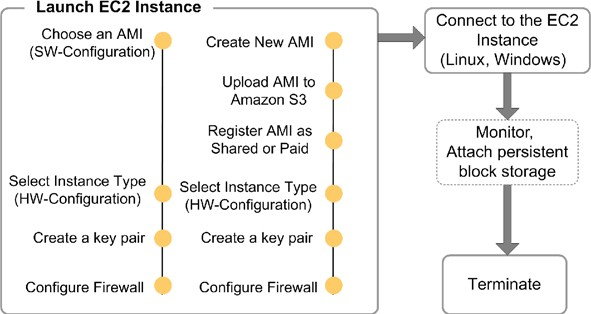
\includegraphics[scale=1]{gambar25.jpg} \\
\textbf{Gambar  2.5} Launch EC2 Instance 
\end{center}
Selain itu mereka dapat dengan cepat menambahkan satu fitur seperti yang disebutkan di atas untuk konfigurasi sesuai  dengan apa yang pengguna inginkan.\\\\
\textbf{GoGrid.}\\\\
GoGrid memiliki  karakteristik umumdengan Amazon di area klasik komputasi  awan,  dalam hal ini mendukung beberapa sistemoperasi melalui gambaran manajemen sendiri, dan mendukung dalamhal menyeimbangkan beban, penyimpanan awan, dan sebagainya. Selain itu, GoGrid menyediakan pelanggan dengan antarmuka web yang user-friendly service, mudah dimengerti demonstrasi video, dan sistempenagihan yang ketat tapi tidak  mahal.\\
Jadi baik EC2 dan GoGrid, kedua-nya menyediakan fitur dasar dan umum dari \textit{Cloud} Computing. Perbedaan antara layanan yang mereka(EC2 dan  GoGrid)  berikan  terutama berasal dari model bisnis mereka masing-masing.\\
Sebagai contoh, GoGrid menyediakan awan(\textit{Cloud}) bebas dan penyimpanan yang spesifik, sedikit berbeda dari Amazon.\\
\tab GoGrid juga menyediakan Hybrid Hosting, yang merupakan fitur pembeda. Banyak aplikasi namun tidak dapat berjalan dengan baik di lingkungan server yang murni  multi-tenant.\\
Performa Database lebih baik pada dedicated server, dimana EC2 dan GoGrid tidak perlu bersaing untuk input / output sumber daya, situasi ini mirip dengan aplikasi web server. GoGrid menyediakan aplikasi-aplikasi khusus dengan dedicated server  yang memiliki  jaminan keamanan yang tinggi.\\\\
\textbf{\textit{Amazon Simple Storage Service (S3).}}\\\\
Amazon Simple Storage Service (2010) (S3) adalah layanan web penyimpanan online yang ditawarkan oleh Amazon Web Services. S3 dapat diakses pengguna melalui layanan web, REST-style interface HTTP, atau dengan melibatkan antarmuka SOAP. Seperti halnya layanan komputasi awan lainnya, pengguna dapat meminta penyimpanan dalamjumlah kecil atau besar dengan cepat, serta menyediakan sistempenyimpanan sangat  terukur.\\
\tab Amazon S3 mengatur ruang penyimpanan ke dalam banyak kotak, dengan setiap kotak diberi namespace yang pada umunya unik dengan maksud untuk membantu menemukan  alamat data, mengidentifikasi \textit{user account} untuk pembayaran, dan mengumpulkan informasi penggunaan. Amazon S3 berurusan dengan semua jenis data sebagai obyek. Sebuah objek dapat diakses melalui URL yang terdiri dari kunci dan versi ID dengan \textit{namespace} sebagai awalan.\\
Pengguna Amazon S3 tersebar di banyak bidang, misalnya, SmugMug, Slideshare dan Twitter. Twitter menggunakan Amazon S3 untuk \textit{host images}, Apache Hadoop menggunakan S3 untuk menyimpan data komputasi, dan utilitas sinkronisasi online seperti Dropbox dan Ubuntu One gunakan Amazon S3 sebagai  tempat penyimpanan dan fasilitas transfer.\\\\
\textbf{\textit{Rackspace Cloud.}}\\\\
Rackspace Awan awalnya diluncurkan pada tanggal 4 Maret 2006 dengan nama "Mosso". Dalam tiga tahun berikutnya, ia(\textit{Raskspace Cloud}) telah mengubah namanya dari "Mosso LLC" menjadi "Mosso: \textit{The Hosting Cloud}", dan akhirnya menjadi "\textit{Rackspace Cloud}" pada  tanggal  17 Juni 2009.\\
\tab Perusahaan  ini  menyediakan layanan  termasuk   \textit{Cloud server},   \textit{Cloud  file},   dan  \textit{Clousite}. \textit{Cloudfile service} adalah layanan penyimpanan awan\textit{(cloud)} yang menyediakan penyimpanan  online yang tak  terbatas  dan  Jaringan Pengiriman  Konten  untuk media  secara komputasi utilitas. Selain control panel online, perusahaan ini menyediakan layanan API\textit{(Application Programming Interface)} yang dapat diakses melalui \textit{Application Programming Interface} yang aman dengan kode klien \textit{open source}.\\
Rackspace memecahkan masalah keamanan dengan mereplikasi tiga salinan penuh data di beberapa komputer pada beberapa zona, dengan setiap tindakan yang dilindungi oleh SSL\textit{(Secure Socket Layer)}.\\\\
\textbf{\textit{Google App Engine.}}\\\\
\textit{Google App Engine} (GAE) tujuan utama adalah untuk mengefisienkan pengguna menjalankan aplikasi web. Seperti yang ditunjukkan pada gambar berikut.\\
\begin{center}
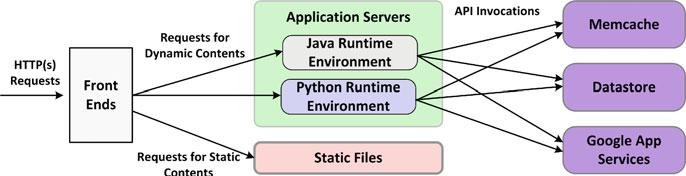
\includegraphics[scale=1]{gambar26.jpg} \\
\textbf{Gambar  2.6} Arsitektur dari \textit{Google App Engine}
\end{center}
\textit{Google App Engine} mempertahankan \textit{Python} dan lingkungan runtime Java  pada  server aplikasi, bersama dengan beberapa \textit{Application Programming Interface} sederhana untuk mengakses layanan Google.\\
\tab Selanjutnya menyebar permintaan HTTP dengan load balancing dan  routing  strategi yang didasarkan pada \textit{Contents}(isi). Runtime sistem yang berjalan pada aplikasi server yang ideal dengan pengolahan logika aplikasi dan menyediakan konten web dinamis, sedangkan halaman statis dilayani  bersama oleh infrastruktur Google.\\
Untuk memisahkan data terus-menerus dari server aplikasi, GAE ( \textit{Google App Engine} ) menempatkan data ke dalam Datastore dari sistem file lokal. Aplikasi dapat mengintegrasikan layanan data dan \textit{Google App} Layanan lainnya, seperti email, penyimpanan  foto  dan sebagainya melalui API ( \textit{Application Programming Interface} ) yang disediakan oleh GAE ( \textit{Google App Engine} ).\\
Selain layanan, Google juga menyediakan beberapa tool untuk pengembang dalam hal ini membantu mereka (pengembang) membangun aplikasi web dengan mudah di GAE (\textit{ Google App Engine} ). Namun, sejak mereka (pengembang) erat terhubung ke infrastruktur Google, ada beberapa pembatasan yang membatasi fungsionalitas dan portabilitas dari  aplikasi.\\
\textbf{Microsoft Azure.}\\\\
Strategi awan Microsoft adalah untuk membangun sebuah  platform  awan  yang mana pengguna dapat memindahkan aplikasi mereka ke dalam cara yang sempurna, dan memastikan bahwa sumber daya yang dikelola dapat diakses untuk kedua layanan awan tersebut   pada aplikasi lokal.\\
\tab Untuk mencapai ini, Microsoft memperkenalkan Windows Azure Platform (WAP), yang terdiri dari sistem operasi Awan(\textit{Cloud}) yang bernama Windows Azure, dan satu set layanan pendukung, seperti ditunjukan pada gambar  berikut.\\
\begin{center}
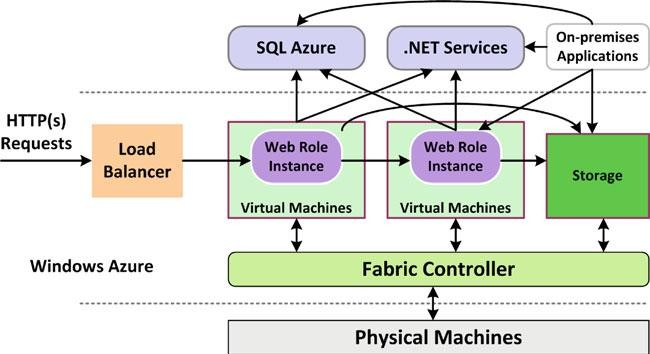
\includegraphics[scale=1]{gambar27.jpg} \\
\textbf{Gambar  2.7} Arsitektur  dari platform Windows Azure
\end{center}
Windows Azure adalah bagian utama dari WAP(\textit{Wireless Application Protocol}). WAP adalah sebuah protokol atau sebuah teknik \textit{messaging service} yang memungkinkan sebuah telepon genggam digital atau \textit{terminal mobile} yang mempunyai fasilitas WAP, melihat/membaca isi sebuah situs di internet dalam sebuah format teks khusus.\\
Ini mempekerjakan mesin virtual sebagai lingkungan runtime nya. Penawaran Aplikasi dalam awan Microsoft dibagi menjadi dua jenis: instansi peran Web, yang dapat melayani permintaan web melalui layanan informasi internet; dan instansi peran pekerja, yang hanya dapat menerima pesan dari instansi peran Web lain atau aplikasi lokal. Windows Azure  mempekerjakan "controller kain" untuk mengelola semua mesin virtual dan server penyimpanan pada mesin fisik di pusat data Microsoft.\\
\tab Windows Azure menggunakan sebuah pengendali kontrol untuk  mengelola  semua mesin virtual dan server penyimpanan pada mesin fisik di pusat data Microsoft. Serupa dengan Datastore di GAE(\textit{Google Application Engine}),WAP(\textit{Wireless Application Protocol}) juga menyediakan layanan database yang disebut SQL Azure, untuk menyimpan data di  awan(\textit{cloud}). Salah satu fitur dari SQL Azure adalah menyediakan alat untuk sinkronisasi data dilokasi lokal.\\
Layanan infrastruktur didukung oleh WAP melalui layanan .NET yang saat ini include dengan kontrol akses dan layanan ekspos. Keduanya tersedia untuk layanan \textit{Cloud}dan layanan lokal.\\
Berikut ini ada 11 top open-source \textit{Cloud}application yang diambil dari GigaOm untuk keperluan pelayanan, pendidikan, support, general itemof interest, dan  lainya.\\
\begin{enumerate}
\item Eucalyptus. Ostatic menggemparkan berita dimana UC Santa Barbara membuat sebuah open-source \textit{Cloud}project tahun kemarin. Dikeluarkan sebagai open-source (dengan menggunakan lisensi FreeBSD-style) Eucalyptus dapat digunakan untuk infrastruktur \textit{Cloud computing} dalam cluster yang dapat menduplikasi fungsionalitas Amazon EC2, Eucalyptus secara langsung menggunakan command-line tool dari Amazon. Sebagai langkah awal Eucalyptus System terlebih dahulu membuat venture funding, untuk  membiayai  staff termasuk arsitek dari Eucalyptus project. Baru baru ini mereka mengeluarkan update software framework nya, yang juga dilengkapi dengan fitur \textit{Cloud computing} yang akan digunakan pada Linux Ubuntu versi terbaru.
\item \textit{Red Hat's Cloud}. Salah satu pemain open-source terlama Red Hat memang telah memfokuskan diri pada \textit{Cloud computing}. Pada akhir juli kemarin,  Red  Hat  membuka sebuah Open Source \textit{Cloud computing} Forum, yang berisi banyak persentasi mengenai ide perpindahan dari open-source untuk mengikuti teknologi cloud.  Anda  dapat  mengikuti  semua free webcast dari semua persentasi Redhat. Pembicaranya Rich Wolski (CTO dari Eucalyptus Systems), Brian Stevens (CTO dari Red Hat), dan juga Mike Olson (CEO dari Cloudera). Steven akan membawa anda mengenai strategi Red Hat terhadap \textit{Cloud computing}. Novell juga open source sedang mencoba untuk memfokuskan ke \textit{Cloud computing}, anda juga dapat  membaca strategi mereka disini.
\item Traffic Server. Yahoo kali ini berpindah ke open-source untuk memberikan inisiatif untuk mewujudkan \textit{Cloud computing} dengan memberikan donasi ke produk \textit{Traffic Server} kepada \textit{Apache Software Foundation}. \textit{Traffic Server} adalah sebuah sistem yang digunakan secara in-house oleh Yahoo untuk mengatur traffic mereka sendiri, dengan ini mereka dapat mengatur \textit{session management, authentication, configuration management, load balancing}, dan juga routing untuk semua \textit{Cloud computing software stack}. Dengan kata lain \textit{Traffic Server} memberikan kemudahan bagi para \textit{IT} administrator untuk mengalokasikan sumber daya, termasuk didalamnya menghandle ratusan dari \textit{virtualized services} secara online.
\item Cloudera. Sebuah \textit{open-source Hadoop software framework} yang saat ini mulai banyak di gunakan pada \textit{Cloud computing deployment} karena fleksibilitas nya yang tinggi dan menggunakan \textit{cluster-based, data-intensive queries tools }ini jadi banyak disukai. Tentu saja ini terlewat oleh I, dan Yahoo juga memiliki \textit{time-tested Hadoop distribution} sendiri. Cloudera nampaknya saat ini menjajikan untuk tahap awal yang memberikan support komersil  untuk Hadoop. anda dapat  membaca tentan Cloudera disini.
\item Puppet. Adalah sebuah teknolosi Virtual server yang dapat di implemetasikan pada \textit{Cloud computing}, dan juga dapat digunakan sebagai \textit{Reductive Lab open-source software} (kurang faham maksudnya apa), software ini dibangun dengan menggunakan \textit{Cfengine system}, dan hebatnya banyak system administrator yang memanfaatkan software ini . Anda dapat dengan mudah mengatur berapapun jumlah virtual machine dan dapat melakukan  automated routine, tampa harus melakukan \textit{complex scripting}.
\item Enomaly. Adalah \textit{Elastic Computing Platform} (ECP) yang merupakan akar dari \textit{ Enomalism open-source provisioning and management software}, teknologi ini di desain untuk mengatur kompleksitas dari implementasi infrastruktur cloud.  ECP  adalah  sebuah  programmable virtual \textit{Cloud computing} infrastructure untuk ukuran kecil, sedang dan juga enterprise besar dan anda dapat  membaca lebih detail disini.
\item 7.	Joyent. Adalah sebuah software yang didirikan pada Januari awal tahun ini, yang memulai open-source  \textit{Cloud} dengan  memanfaatkan  JavaScript  dan  Git.  Infrastruktur  Joyent  cloudhosting dan \textit{Cloudmanagement software} membuka banyak open-source tools untuk public dan private cloud. Perusahaan ini juga membantu mengoptimasi kecepatan  implementasi dari open-source MySQL database untuk penggunaan \textit{Cloud use}.
\item Zoho. Banyak orang mengenal Zoho sebagai free, \textit{online application}, yang menjadi pesaing dari Google Docs. Yang terpenting untuk diketahui adalah bawasanya Zoho core adalah betul betul open source mdash; sebuah contoh bagaimaa solusi SaaS dapat  bekerja  secara harmonis dengan open source. Anda dapat menemukan bagaimana Zoho mengimplementasikan open-source tool melalui interview  mereka.
\item Globus Nimbus. Open-source toolkit ini mampu merubah bisnis anda dari infrastruktur  cluster menjadi Infrastructure-as-a-Service (IaaS) cloud. Amazon EC2 interface digunakan sepenuhnya namun ini bukan hanya sebuah interface yang dapat anda manfaatkan.
\item Reservoir. Adalah sebuah inisiatif dari European research  untuk  mengembangkan virtualized infrastructure and \textit{Cloud computing}. Akhirnya membawa mereka untuk mengembangkan teknologi open-source untuk \textit{Cloud computing}, dan membantu para pengguna bisnis untuk menghemat  biaya IT.
\item OpenNebula. OpenNebula VM Manager adalah sebuah komponen dasasr dari Reservoir. Ia adalah sebuah jawaban open-source untuk berbagai macam jenis virtual machine management yang banyak di gunakan secara proprietary, Interface nya pun dapat dengan mudah dipahami dengan \textit{Cloud infrastructure tools and services}.  "OpenNebula  adalah sebuah open-source virtual infrastructure engine yang akan memberikan anda implementasi dan re-placement dari virtual machines pada physical resources," menurut project lead mereka.
\end{enumerate}
Nampaknya banyak \textit{open-source tools} sudah mulai berkompetisi dalam dunia \textit{Cloud computing}. Hasil akhir dari ini tentu saja nantinya kita akan menemukan fleksibilitas dari organisasi untuk mengkostumasi pendekatan yang mereka inginkan. Open-source \textit{Cloud}akan  memberikan potensi akan harga yang sangat kompetitif  untuk mendapatkan service cloud.
\section{Manajemen  Pengelolaan \textit{Cloud computing}}
Secara teori, sumber daya awan-berbasis layanan tidak harus berbeda dari sumber daya di lingkungan dimana kita berada. Idealnya, Anda memiliki pandangan yang lengkap dari sumber daya yang Anda gunakan saat ini atau mungkin ingin menggunakan di masa depan, namun untuk mencapai ini bukan merupakan sesuatu yang mudah. Dalam lingkungan awan(\textit{cloud}) kebanyakan, pelanggan hanya dapat mengakses layanan, yang berhak mereka  gunakan.\\
Tiga aspek manajemen sumber daya awan(\textit{Cloud Computing}):\\
\begin{itemize}
\item Keamanan TI
\item Kinerja manajemen
\item Provisioning
\end{itemize}
\textbf{Kinerja Manajemen.}\\\\
Manajemen kinerja adalah tentang bagaimana layanan perangkat lunak berjalan efektif  di  dalam lingkungan sendiri(PC sendiri) ataupun melalui awan(\textit{Cloud}). Jika Anda mulai dapat terhubung dengan perangkat lunak yang berjalan di pusat data, lalu Anda sendiri langsung ke perangkat lunak yang berjalan di awan(\textit{Cloud}), kemungkinan besar Anda akan ada potensi kemacetan pada titik koneksi.\\\\
\textbf{Jasa manajemen}\\\\
Jasa manajemen dalamkonteks ini mencakup semua kegiatan operasi data \textit{centre}.\\
Disiplin yang luas ini mempertimbangkan teknik yang diperlukan dalam manajemen \textit{Cloud Computing} dan alat untuk mengelola jasa/layanan oleh penyedia awan(\textit{Cloud}) dan data internal manajer pusat di lingkungan ini, hal –hal yang diperlukan antara lain:\\
\begin{itemize}
\item Fisik
\item TI
\item Virtual
\end{itemize}
Layanan manajemen mencakup berbagai  disiplin,  yaitu :\\
\begin{itemize}
\item Konfigurasi  manajemen
\item Aset Manajemen
\item Jaringan manajemen
\item Kapasitas  perencanaan
\item Analisis akar penyebab
\item Beban Kerja manajemen
\item Patch dan memperbarui manajemen
\end{itemize}
Namun Kenyataannya adalah bahwa \textit{Cloud}itu sendiri adalah sebuah platform manajemen layanan. Oleh karena itu, portofolio layanan \textit{Cloud}dirancang dengan baik  termasuk integrasi ketat dari  kemampuan layanan manajemen inti dan antarmuka yang terdefinisi dengan baik.\\\\
\textbf{Mengelola beban kerja di Awan ( \textit{Cloud})}\\\\
Bagaimana Anda mengatur Teknologi ini (\textit{cloud})? Persyaratan dasar adalah bahwa beban kerja perlu untuk diorganisir.Beban kerja adalah sebuah layanan independen atau kumpulan kode yang dapat dieksekusi.\\
Oleh karena itu, beban kerja tidak perlu bergantung pada unsur luar. Beban kerja bisa menjadi sebuah aplikasi kecil atau lengkap. Dimana kita harus dapat menyeimbangkan dua hal:\\
\begin{itemize}
\item Aplikasi atau komponen yang berjalan di awan(\textit{cloud})
\item Kebutuhan bisnis untuk melakukan perkiraan /estimasi kebutuhan bisnis, terutama saat beban puncak.
\end{itemize} 
Organisasi harus secara aktif mengelola beban kerja sehingga mereka tahu\\
\begin{itemize}
\item Bagaimana aplikasi  mereka berjalan
\item Apa yang mereka lakukan
\item Berapa banyak departemen individu atau UKM harus dikenakan biaya untuk setiap penggunaan layanan \textit{Cloud computing}
\end{itemize}
\tab Setiap provider layanan \textit{Cloud computing} dalam menjalankan jasa bisnis-nya membutuhkan suatu perencanaan untuk beban kerja mereka, bahkan  ketika  perusahaan layanan tersebut sedang menggunakan operator eksternal Cloud. Manajemen perlu memahami jenis beban kerja mereka untuk ditempatkan di \textit{Cloud}.\\
Beban kerja bisa menjadi segalanya dari data intensive untuk penyimpanan beban kerja atau proses transaksi  beban kerja.\\
\tab Hal yang perlu diperhatikan dalammanajemen pengolahan \textit{Cloud computing} adalah
"Mendeklarasikan Jenis Data", jumlah data yang tersedia untuk digunakan Perusahaan yang menggunakan layanan \textit{Cloud}sangatlah banyak dan sifat datanya berubah,  meliputi :\\
\begin{itemize}
\item Keragaman data meningkat\\
Data dalam\textit{Cloud computing} menjadi lebih beragam, selain data "tradisional" terstruktur (pendapatan, nama dan sebagainya) termasuk email, gambar,  blog dan lain-lain.
\item Jumlah data meningkat\\
Coba pikirkan berapa banyak pengelolaan video You Tube atau dapat menangani semua gambar. Bahkan dalam pemakaian data tradisional, bidang, organisasi yang memakai data tersebut jumlah agregatnya mulai besar.
\item Latency persyaratan menjadi lebih  menuntut. 
Perusahaan-perusahaan  semakin menuntut latency yang lebih rendah (misalnya, waktu untuk mendapatkan data dari satu titik ke titik lainnya) untuk banyak aplikasi.
\end{itemize}
Dengan demikian  \textit{Cloud}dapat :\\
\begin{itemize}
\item Menyediakan sumber daya untuk mengakses permintaan data dengan harga  yang  jauh lebih rendah.
\item Mendukung bisnis dalam penggunaan data secara kolaboratif ( seluruh  karyawan, pelanggan dan mitra bisnis.
\end{itemize}
\textbf{Penyelengara Jasa \textit{Cloud}}\\\\
\tab Dalam penyelengaraan jasa \textit{Cloud computing}, Perusahaan yang menyelengarakan teknologi  ini sudah seharusnya bertanya pada diri sendiri dengan pertanyaan:\\
\begin{itemize}
\item Layanan \textit{Cloud}seperti  apakah yang user mau dari penyedia layanan Cloud?
\item Bagaimana "kita" tahu apakah kinerja dari\textit{Cloud computing} yang diberikan atau ditawarkan kepada user berada pada tingkat yang tepat?
\item Bagaimana "kita" bisa menilai apakah data yang telah dihapus benar-benar hilang?
\end{itemize}
Mengelola biaya \textit{IT}\\\\
Semua departemen \textit{IT} memonitor biaya, tetapi hanya sedikit dari   "mereka" yang memantau dalam hal aset kinerja - keharusan untuk mengoptimalkan hasil investasi baik untuk hardware dan software.\\
Hal ini mungkin berubah dengan munculnya layanan \textit{Cloud}, tidak seperti model lisensi tradisional, proposisi \textit{Cloud}di  dasarkan pada pengaturan sewa.\\
Anda harus membandingkan dua model biaya :\\
\begin{enumerate}[label=\alph*]
\item Beban usaha (membayar per bulan,  per pengguna untuk setiap layanan)
\item Modal investasi (membayar biaya beli ditambah pemeliharaan tahunan untuk perangkat lunak yang berada dalamorganisasi  Anda - sebagai pengguna).
\end{enumerate}
Ada beberapa hal yang harus dipertimbangkan user sebagai pengguna layanan \textit{Cloud computing},  terkait manajemen pengelolaan \textit{Cloud}:\\
\begin{itemize}
\item Apakah vendor  bersedia untuk memecahkan masalah Anda(user) ?
\item Seberapa efektif  penyedia dalammengelola lingkungan mereka sendiri ?
\item Apakah vendor  menyediakan layanan berulang ?
\item Bagaimana vendor menangani sebuah outage ?
\item Apa pengalaman vendor dalammenangani  masalah pelanggan ?
\end{itemize}
\textbf{Pengantar  Manajemen Penyimpanan.}\\\\
\tab Salah satu tren komputasi terbesar dalam komunitas bisnis adalah konsep jaringan komputasi awan. Ketika tenaga teknis dan manajemen menggunakan istilah "awan," mereka berbicara mengenai  solusi jaringan berbasis internet.\\
Desain adalah memberikan layanan on demand ke pengguna akhir, tanpa mengharuskan mereka untuk memiliki  keahlian teknis untuk mendukung layanan tersebut.\\
Arsitektur lingkungan komputasi awan agak sederhana secara keseluruhan,  meskipun  komponen individu mungkin sangat kompleks. Ini terdiri dari tiga bagian yang berbeda. Infrastruktur IT adalah data center, di mana informasi klien diproses dan disimpan.\\
Sisi lain dari arsitektur awan adalah lingkungan klien.  Antara keduanya  adalah awan(\textit{cloud}):  satu set kontrol untuk melindungi, mengelola, dan mendistribusikan akses dari lingkungan klien ke infrastruktur TI. Bagaimana tiga bagian yang dibangun didasarkan pada kebijakan, prosedur, dan perangkat keras yang digunakan oleh pihak administrasian.\\
Tidak peduli bagaimana lingkungan komputasi awan terlihat, konsep ini adalah untuk memberikan kemampuan IT "sebagai layanan." Dimana Layanan-layanan  tersebut  dapat berupa aplikasi web yang dapat diakses, manajemen file, dan penyimpanan data. Dari semua layanan ini, yang terbesar dan paling populer adalah \textbf{manajemen penyimpanan}.\\
Untuk kebanyakan bisnis, penyimpanan adalah yang paling penting dan paling mahal sumber daya \textit{IT} dalam infrastruktur mereka. Sayangnya, tenaga ahli yang bertugas untuk manajemen penyimpanan tidak konsisten dengan kebutuhan yang diperlukan.\\
Manajemen Penyimpanan adalah kemampuan untuk menyimpan dan mengatur file dan data pada jaringan. Perangkat lunak yang digunakan untuk memastikan kemampuan ini disebut \textit{Storage Resource Management } (SRM).\\
Perhatian utama untuk manajemen penyimpanan adalah kapasitas, penggunaan, kebijakan dan manajemen "peristiwa". Dalam penyimpanan komputasi awan, tujuannya adalah kemampuan berpikir Internet untuk   mengakses penyimpanan.\\
\tab Berbicara mengenai manajemen pengolahan \textit{Cloud Computing}, secara otomatis  kita akan membahas juga tentang manajemen keamanan pada \textit{Cloud Computing} ditinjau dari orang atau individu.\\
Salah satu tindakan yang paling penting bagi tim keamanan adalah untuk mengembangkan sebuah penyewaan formal bagi organisasi keamanan dan program. Ini akan menumbuhkan visi bersama antara tim yang menuju pada suatu pengharapan bersama mengenai jaminan keamanan data yang diatur secara baik dan benar demi  berlangsungnya proses pengolahan data dengan manajemen yang baik di dalam layanan \textit{Cloud}. Penyewaan harus diselaraskan dengan rencana strategis organisasi  atau perusahaan tersebut  bekerja untuk timkeamanan.\\
Kurangnya peran dan tanggung jawab yang jelas, dan kesepakatan tentang harapan, dapat mengakibatkan kehilangan dan kerancuan antara tim keamanan tentang apa yang diharapkan dari mereka, bagaimana ketrampilan / kemampuan mereka dan pengalaman yang bertambah dan memenuhi  tujuan kinerja mereka.
\section{Sumber  Daya Manusia \textit{Cloud computing}}
Memahami "pemain" dalamlingkungan komputasi awan adalah hal yang penting untuk lebih memahami cara kerja yang lebih dalamdari penyedia platform, untuk kelangsungan bisnis atau individu.\\
Berikut ini adalah sumber daya manusia yang terlibat dalam Komputasi Awan  (\textit{Cloud Computing}) :
\begin{itemize}
\item \textbf{Subscribers (Pelanggan).}\\
Kelompok ini terdiri dari pebisnis yang menggunakan penawaran  platform-as-a-service untuk mengembangkan dan menyebarkan aplikasi mereka. Dimana mereka mencari penawaran \textit{Cloud}yang tepat untuk menjalankan usaha mereka, sehingga mempermudah mereka dalam berbisnis, menekan biaya usaha, efisien waktu dapat mereka peroleh  dengan menggunakan  penawaran ini.
\item \textbf{Publishers (Penerbit).}\\
Ketika pelanggan mulai menggunakan suatu penawaran, mereka sering memiliki akses ke katalog global dari aplikasi yang diterbitkan, alat-alat, prasarana, dan platform yang meningkatkan atau memperluas penawaran asli. item yang ditemukan di katalog disediakan oleh penerbit. Dalam dunia bisnis, perusahaan dapat berlangganan ke layanan ini, sementara para pengembang mempublikasikan   layanan tersebut.
\item \textbf{Operator  Pusat  Data (Data Center Operators).}\\
Se-golongan dengan penerbit (dan yang utama untuk menawarkan) adalah operator pusat data yang menyediakan server, penyimpanan, dan konektivitas jaringan untuk platform.
\item \textbf{Vendor untuk layanan Web Terpadu (Vendors for Integrated Web Services).}\\
Berbagai layanan yang tersedia di Internet, banyak yang mungkin tidak disertakan dalam katalog global karena layanan tersebut diasumsikan atau karena popularitas mereka atau karena pelayanan yang belumdipublikasikan ke dalam catalog.\\
\item \textbf{Penyedia Jasa OutSource (Providers for  Outsourced Services).}\\
Selain operator pusat data yang mendukung infrastruktur aplikasi, beberapa kegiatan lain untuk mengembangkan dan mengelola aplikasi dapat dikelola oleh sumber daya lain, biasanya melalui  \textit{outsourcing} pekerjaan.
\item \textbf{Klien (Clients).}\\
Klien adalah pengguna internet yang dapat mengakses sumber daya yang diterbitkan.
\end{itemize}
\textbf{Sponsor   \textit{Cloud}(Awan)  adalah Pelanggan}\\\\
Sebagian besar percakapan ditemukan di media adalah berbicara tentang manfaat komputasi awan dan  penawaran \textit{platform-as-a-service}.\\
Keuntungan yang ditemukan berkisar dari pengurangan biaya dengan kemampuan  aplikasi  yang memiliki konektivitas yang lebih baik. \textit{Cloud computing}  pasti  memiliki  banyak  manfaat yang tersedia bagi orang-orang yang mengambil keuntungan dari itu. Yang menjadi pelanggan seringkali diwajibkan untuk mengakses layanan  utilitis  berbasis  komputasi. Dalam berlangganan perlu terlebih dahulu melakukan Pendaftaran, dan dalam proses pendaftaran memerlukan biaya pendaftaran dari pihak-pihak yang ingin  berlangganan.  Pihak  –pihak tersebut mungkin dari perorangan untuk platform sosial, atau untuk usaha kecil dan menegah, Web 2.0 dan perusahaan SaaS, dan perusahaan besar  untuk platformlainnya.\\
\tab Kebanyakan pelanggan mencari utilitas berbasis platform untuk meringankan beban pemilik dan mengelola server, pusat data, jaringan, atau apapun yang terkait dengan penunjang infrastruktur komputasi. Dengan berlangganan mereka dapat menyebarkan  aplikasi, mendapatkan skala aplikasi secara dinamis, atau memberikan hak akses ke  aplikasi  dari seluruh dunia. Mereka dapat menggunakan platform ini secara permanen atau untuk menutup beban kerja yang berlebihan atau proyek tertentu secara temporer.\\
\tab Karena pelanggan memiliki tanggung jawab untuk melakukan pembayaran atas penggunaan platform, mereka biasanya memiliki tujuan bisnis yang spesifik dan memenuhi tujuan tersebut.\\
Platform yang mereka pilih harus mampu memenuhi tujuan bersama mereka, baik  jangka pendek maupun jangka panjang dengan pengurangan biaya yang disediakan oleh langganan platform-as-a-service mereka. Tujuan ini berkisar, menyadari manfaat dari fleksibilitas dan skalabilitas dari komputasi awan untuk mendapatkan "kepemimpinan" pasar melalui   konsep global positioning di Internet.\\
Pelanggan bergantung pada penerbit untuk memastikan bahwa layanan yang dibeli dimanfaatkan secara efektif dan efisien, dan apapun yang digunakan klien dipublikasikan di platform. Dalam banyak kasus pelanggan memiliki akses ke segala sesuatu yang diterbitkan di dalamplatform \textit{Cloud}.\\\\
\textbf{Pembuatan \textit{Cloud}: Penerbit.}\\\\
Penerbit membuat kompilasi dari vendor untuk perangkat lunak independen, peralatan virtual, infrastruktur, platform, dan peralatan. vendor dapat mempublikasikan peralatan, arsitektur siap pakai dan aplikasi. Apapun yang dibuat vendor ditemukan dalam sebuah katalog global. Setiap \textit{platform-as-a-service} memiliki katalog global mereka sendiri, meskipun beberapa  item seperti Web API(\textit{Application Programming Interface}) dan plug-in pada umunya dapat ditemukan dalam beberapa katalog. Penerbit dapat menentukan pelanggan mana yang memiliki akses ke item yang di publikasikan dan berapa harga-nya. ini pasti bermanfaat bagi platform sosial yang dibangun berdasarkan kontribusi berbagai penerbit. Untuk platform yang fokus pada aplikasi bisnis, penerbit dapat membagi kode aplikasi  dengan  penerbit  lain atau menyediakan  produk jadi kepada klien.\\
\tab Mayoritas penerbit adalah pengembang aplikasi. Mereka bisa membangun aplikasi yang mendukung pelanggan tertentu, untuk digunakan oleh pelanggan lain, untuk digunakan oleh pengembang lain dalam rangka meningkatkan atau memperluas aplikasi mereka untuk penerbitan, atau untuk pelanggan komersial. Aplikasi mereka mungkin gratis atau ber-bayar. Dalam beberapa platform seperti Second Life, biaya tersebut mungkin biaya virtual yang hanya berlaku di  dalam platformtersebut.\\
\tab Jenis lain dari penerbit dapat ditemukan di dalam Internet. Vendor alat perangkat keras dapat membuat perangkat lunak virtual setara dengan peralatan mereka, seperti firewall, \textit{load balancers}, peralatan keamanan dan sejenisnya. Vendor dari platform dan \textit{middleware} mempublikasikan paket perangkat lunak yang siap digunakan tanpa instalisasi atau konfigurasi yang canggih. Bahkan semua arsitektur dapat ditemukan di internet dan diumumkan oleh para ahli professional.\\
Penerbit mengandalakan operator pusat data untuk mempertahankan sebuah platform yang handal, terukur dan aman serta memelihara katalog global. Klien dan pelanggan yang menggunakan  produk yang diterbitkan penerbit  memberikan  umpan  balik langsung  pada  nilai produk mereka.bagi banyak penerbit umpan balik ini mungkin dalam bentuk pendapatan. Untuk produk yang gratis, umpan balik mungkin dalam hal popularitas. Setiap aplikasi, alat, layanan, atau bahkan situs Web ditemukan di Internet dan disampaikan oleh penerbit. Tanpa penerbit, World Wide Web tidak akan ada.\\\\
\textbf{Pendukung \textit{Cloud computing} : Operator Pusat Data.}\\\\
Setiap menawarkan utilitas yang berbasis sekelompok individu untuk memastikan bahwa infrastruktur yang mendukung penawaran berfungsi seperti yang diharapkan dan menangani masalah tak terduga yang mungkin timbul. Kegiatan ini adalah inti dari apa yang disebut manajemen data center dan orang yang mendukung proses ini adalah operator pusat data.\\
Kelompok ini sebagian besar transparan untuk operasi. Perwakilan Dukungan pelanggan mungkin tersedia untuk pertanyaan dan pelaporan masalah. Namun orang-orang ini adalah bagian kecil dari operator pusat data. Mayoritas kelompok ini memiliki tanggung jawab langsung terikat pada pemeliharaan server, perangkat penyimpanan, koneksi  jaringan,  perangkat  lunak dan alat-alat.\\
\tab Operator pusat Data adalah bentuk khusus dari penerbit: apa yang mereka terbitkan adalah infrastruktur yang besar untuk menangani hosting, mengatur layanan, pusat data perusahaan, serta layanan lainnya. Sebagai penerbit, mereka menentukan harga untuk sumber daya yang mereka sediakan , siapa yang dapat menggunakan sumber daya tersebut, dan dalambeberapa kasus bagaimana sumber  daya tersebut akan digunakan.\\
Tujuan dari operator pusat data adalah untuk mempertahankan keandalan, ketersediaan, dan keamanan infrastruktur. Sejak infrastruktur \textit{Cloud}sebagian besar adalah virtualisasi operator ini bertanggung jawab untuk menerapkan dan memelihara setiap kontrol virtual yang diperlukan. Mereka mengatur konfigurasi dan kontrol otomatisasi untuk memungkinkan sejumlah  fitur jaringan dari keseimbangan beban kerja, replikasi, dan penyimpanan  cadangan.\\
\tab Operator pusat data bergantung pada orang dan bisnis yang menggunakan infrastruktur. Beberapa layanan utilitas sudah banyak yang menggunakannya disamping  bisnis  utama mereka .Provider seperti Amazon.com, IBM, EMC2, dan Google memiliki bisnis inti  yang  berhasil  sebelummenawarkan layanan utilitas.\\\\
\textbf{Vendor untuk Integrated Services Web.}\\\\
Layanan Web yang diintegrasikan ke dalam penawaran platform dapat bermanfaat bagi semua pelanggan. Biasanya layanan web ini tidak ditawarkan oleh pelayanan ini, tetapi dibuat ada  oleh layanan yang  bersangkutan.  Sumber  layanan  web  berasal dari  serangkaian  vendor yang telah mengembangkan layanan ini secara khusus. World Wide Web konsorsium mendefinisikan layanan web sebagai "sistem software yang didesain untuk mendukung mesin yang dioperasikan dengan interaksi mesin melalui jaringan". Layanan web yang paling umum adalah dalam bentuk akses API (\textit{Application Programming Interface}) Web melalui Internet atau jaringan apapun dan dijalankan pada sistemremote host  layanan tersebut.\\
\tab Jasa tersebut biasanya terbagi dalam dua kategori: \textit{Big Web Services} dan \textit{RESTful Web Services}. \textit{Big Web Services} menggunakan standar SOAP untuk membangun / membuat pesan XML. Layanan ini menjadi populer untuk saat-saat ini Namun, \textit{RESTfulL Web Services} mendapatkan popularitas. Berdasarkan protokol  REST,  layanan Web ini cenderung    melakukan proses integrasi yang lebih baik dengan  HTTP  daripada  layanan  berbasis  SOAP(\textit{Simple Object Access Protocol}). Mereka juga tidak memerlukan penggunaan XML atau WSDL.\\
\tab \textit{Web services} dapat digunakan dalam beberapa cara; tiga yang paling populer adalah RPC, SOA dan REST.\\\\
\begin{enumerate}
\item Remote procedure call (RPC) adalah teknologi antara proses-proses yang memungkinkan atau mengijinkan aplikasi secara jarak jauh menjalankan subrutin atau prosedur di komputer lain dengan berbagi jaringan tanpa pengkodean yang jelas untuk interaksi.
\item Layanan web Arsitektur berorientasi layanan (SOA) didasarkan  pada  arsitektur dan membuat fungsi SOA diakses melalui protokol Internet standar tanpa ketergantungan pada platformatau bahasa pemrograman.
\item Representasi state transfer (REST) adalah jasa / layanan yang meniru protokol dengan membatasi antarmuka untuk seperangkat operasi  standar.
\end{enumerate}
Salah satu layanan Web ini mungkin diperlukan oleh aplikasi dan layanan yang terdapat pada platform. Web services menambahkan komunikasi yang dibutuhkan sebagai nilai tambah untuk sejumlah tugas yang berkaitan dengan penggunaan dan pemantauan aplikasi pada web.  Mereka dapat digunakan oleh perangkat monitoring, penagihan jasa, pelacak transaksi, mesin untuk penyimpanan dan kebijakan,  dan sejenisnya.\\\\
\textbf{Penyedia Jasa Outsource.}\\\\
Dengan manfaat dari utilitas berbasis layanan, memungkinkan perusahaan untuk meringankan keuangan dan beban kerja sehingga bisnis inti dapat difokuskan pada beberapa kegiatan yang masih diperlukan/dibutuhkan oleh bisnis. Ini bisa dari pengembangan aplikasi, untuk memantau aplikasi dalam produksi, untuk mendukung pelanggan dan untuk manajemen aplikasi. Ada beberapa perusahaan jasa teknologi yang telah memberikan keseluruhan manajemen operasional bisnis bagi perusahaan. Hal ini biasanya disebut sebagai operasi yang dikelola dan meliputi seluruh solusi IT. Meskipun komputasi awan telah meringankan banyak beban untuk mengelola solusi IT ;\\
Beberapa perusahaan masih melihat kegiatan outsource untuk manajemen IT ke penyedia lainnya. Mereka mungkin tidak memiliki keahlian atau ketrampilan yang diperlukan untuk mengelolah manajemen, tidak memiliki peralatan yang diperlukan. Atau mereka  hanya  lebih suka tidak mengikat usaha mereka dalamhal-hal tersebut.\\
\section{Model  Keamanan \textit{Cloud computing}}
Komputasi awan telah didefinisikan sebagai penggunaan sekumpulan layanan terdistribusi, aplikasi, informasi dan prasarana terdiri dari komputer, jaringan, informasi dan sumber daya penyimpanan. Komponen-komponen ini dapat dengan cepat diatur,  ditetapkan, diimplementasikan, dan dihentikan dengan menggunakan utilitas  on-demandseperti  model alokasi  dan pemakaian.\\
\tab Penyedia layanan awan memanfaatkan teknologi virtualisasi  yang dikombinasikan dengan kemampuan layanan mandiri untuk menghitung sumber daya melalui Internet. Dalam lingkungan operator selular, mesin virtual dari beberapa organisasi  harus  co-terletak  pada server fisik yang sama dalam rangka untuk memaksimalkan efisiensi  virtualisasi.\\
Penyedia layanan \textit{Cloud} harus belajar dari model penyedia layanan yang dikelola dan memastikan bahwa aplikasi dan data dari pelanggan mereka  aman,  jika mereka  berharap  untuk   mempertahankan   pelanggan   dan   daya   saing.   Saat   ini,   perusahaan   mencari arah cakrawala/wawasan komputasi awan untuk memperluas infrastruktur lokal, tapi kebanyakan  tidak mampu membayar resiko mengorbankan keamanan dari aplikasi  dan  data.  Sebagai contoh, IDC baru-baru ini melakukan survei (lihat Gambar ) dari 244 eksekutif  IT / CIO dan rekan line-of-business (LOB) mereka, untuk mengukur pendapat mereka dan memahami perusahaan mereka dalam menggunakan layanan teknologi awan. Keamanan menduduki peringkat  pertama sebagai tantangan dan masalah besar komputasi awan.(\textit{Cloud  Computing}).\\
\begin{center}
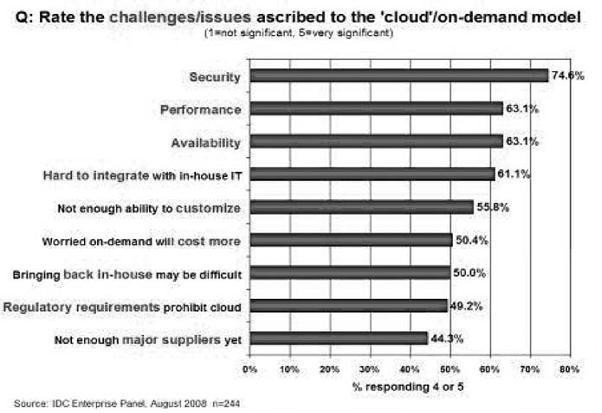
\includegraphics[scale=1]{gambar28.jpg} \\
\textbf{Gambar  2.8} Hasil survey tantangan keamanan IDC(\textit{International Data Corporation})
\end{center}

Terinspirasi oleh pergerakan industri \textit{IT} menuju SaaS, di mana perangkat lunak  tidak  dibeli, tetapi menyewa layanan dari penyedia, \textit{IT-as-a-Service} (ITaaS) sedang diusulkan untuk mengambil konsep ini lebih lanjut, untuk membawa hak model layanan untuk Infrastruktur TI anda. organisasi \textit{IT} modern harus menjalankan dirinya sebagai operasi yang terpisah dan menjadi  lebih strategis dalam pengambilan keputusan operasional.\\
Banyak organisasi dalam proses transformasi departemen IT mereka ke pusat biaya  operasional mandiri, memperlakukan pengguna internal yang seolah-olah mereka adalah pelanggan.\\
\tab Transformasi ini tidak sepele dan biasanya melibatkan unsur-unsur manajemen proyek portofolio, alur kerja rekayasa ulang, dan perbaikan proses. Transformasi ini memerlukan waktu yang lama untuk diselesaikan. Banyak organisasi IT besar yang telah mengadopsi  kerangka kerja \textit{Information Technology Infrastructure Library} (ITIL) dengan maksud membantu melalui trasformasi ini.\\\\
\textbf{Tantangan Keamanan \textit{Cloud}}\\\\
Meskipun virtualisasi dan komputasi awan dapat membantu perusahaan mencapai /melakukan sesuatu yang lebih dengan melanggar ikatan fisik antara infrastruktur \textit{IT} dan penggunanya, ancaman keamanan yang tinggi harus diatasi dalam rangka untuk mendapatkan manfaat sepenuhnya dari paradigma komputasi baru. Hal ini terutama berlaku untuk penyedia SaaS. Beberapa kekhawatiran keamanan adalah diskusi bernilai lebih. Sebagai contoh, di awan, Anda kehilangan kendali atas aset dalam beberapa hal, sehingga model keamanan Anda harus ditinjau kembali. Keamanan yang baik bagi perusahaan adalah yang menjadi mitra, department yang dapat diandalkan atau dipercaya. Dapatkah Anda mempercayai data Anda ke penyedia layanan Anda? Dalam paragraf berikut, kita membahas beberapa isu yang harus Anda pertimbangkan sebelummenjawab  pertanyaan.\\
\tab Dengan model awan, Anda kehilangan kontrol atas keamanan fisik. Dalam awan umum, Anda berbagi sumber daya komputasi dengan perusahaan lain. Di luar perusahaan anda tidak memiliki pengetahuan atau kendali dimana sumber daya dijalankan. Mengekspos data anda dalam lingkungan bersama dengan perusahaan lain , menjadikan "alasan yang masuk  akal" bagi pemerintah untuk menyita aset Anda karena perusahaan lain tersebut telah melanggar hukum. Hanya karena Anda berbagi lingkungan/tempat/ruangan di awan, dapat menempatkan data Anda pada resiko penyitaan/penyerangan.\\
\tab Layanan Penyimpanan yang disediakan oleh satu vendor awan mungkin tidak kompatibel dengan layanan vendor lain namun disatu sisi anda harus memutuskan untuk berpindah dari satu ke yang lain, dalamrangka memenuhi kebutuhan perusahaan anda.\\
Jika informasi dienkripsi saat melewati awan(\textit{Cloud}), siap yang mengontrol kunci enkripsi / dekripsi? Apakah pelanggan atau perusahaan \textit{Cloud} ? kebanyakan nasabah  mungkin  ingin data mereka dienkripsi dengan dua tipe control diatas (pengontrolan oleh pelanggan atau perusahaan \textit{Cloud}) di internet menggunakan SSL (\textit{Secure Sockets  Layer  protocol}).  Mereka juga mungkin ingin data mereka terenkripsi ketika sedang beristirahat di pool penyimpanan perusahaan awan(\textit{Cloud}). Pastikan anda sebagai pelanggan mengontrol kunci enkripsi/dekripsi, sama seperti ketika data masih tinggal di server anda sendiri.\\
\tab Integritas data artinya: memastikan bahwa data yang identik dijaga selama operasi apapun (seperti transfer, penyimpanan, atau pengambilan). Secara sederhana, integritas data adalah jaminan bahwa data konsisten dan benar. Memastikan keutuhan benar-benar dari data berarti bahwa perubahan hanya sebagai respons terhadap transaksi yang berwenang. Ini kedengarannya bagus, tetapi Anda harus ingat bahwa standar umum untuk  memastikan integritas data belum ada. Menggunakan penawaran SaaS di awan berarti bahwa ada sedikit kebutuhan untuk pengembangan perangkat lunak. Jika Anda berencana untuk menggunakan kode yang dikembangkan secara internal di awan(\textit{Cloud}), bahkan lebih penting untuk memiliki siklus pengembangan  perangkat  lunak  yang  aman  secara formal.  Penggunaan "teknologi mashup" yang belum matang (kombinasi layanan web), yang merupakan dasar aplikasi awan (\textit{Cloud}),tanpa disadari akan menyebabkan kerentanan keamanan dalam aplikasi tersebut. Pengembangan alat pilihan Anda , harus memiliki model keamanan yang tertanam/ melekat di dalamnya untuk membimbing pengembang dalam tahap pengembangan dan membatasi user dalampenggunaan data resmi mereka ketika sistemsedang digunakan di dalamproduksi.\\
\tab Aplikasi Awan(\textit{Cloud}) mengalami penambahan fitur yang konstan, dan pengguna harus terus up to date dengan perbaikan aplikasi untuk memastikan bahwa mereka dilindungi. kecepatan aplikasi yang akan berubah dalam awan(\textit{Cloud}) akan  mempengaruhi  SDLC (software    development     life    cycle)dan  keamanan. Sebagai     contoh,     Microsoft SDLC mengasumsikan bahwa misi penting perangkat lunak akan memiliki tiga sampai lima tahun periode dimana ia tidak akan berubah secara substansial, namun Awan (\textit{Cloud}) mungkin memerlukan perubahan aplikasi setiap beberapa minggu sekali. lebih buruk lagi, SLDC yang aman tidak akan mampu memberi siklus keamanan yang terus menerus terjaga dengan perubahan yang terjadi begitu cepat. Ini berarti bahwa pengguna harus terus-menerus upgrade, karena versi lama tidak dapat berfungsi, atau tidak dapat melindungi  data.\\
\tab Disini akan diambil contoh keamanan pada Layanan SaaS (\textit{Software as a Service}). Model \textit{Cloud computing} masa depan kemungkinan besar akan menggabungkan penggunaan SaaS, utilitas komputasi, dan kolaborasi teknologi Web 2.0 untuk memanfaatkan Internet untuk memenuhi  kebutuhan pelanggan mereka.\\
Model bisnis baru yang dikembangkan sebagai hasil dari peralihan ke \textit{Cloud Computing} tidak hanya menciptakan teknologi baru dan proses operasional bisnis tetapi juga persyaratan keamanan baru dan tantangan yang baru. Sebagai langkah evolusi terbaru dalam model layan \textit{Cloud} (seperti gambar di bawah ini), SaaS kemungkinan akan tetap menjadi model layanan awan yang dominan untuk masa yang akan datang dan sebagai tempat kebutuhan yang paling penting untuk praktik keamanan dan pengawasan.\\
\begin{center}
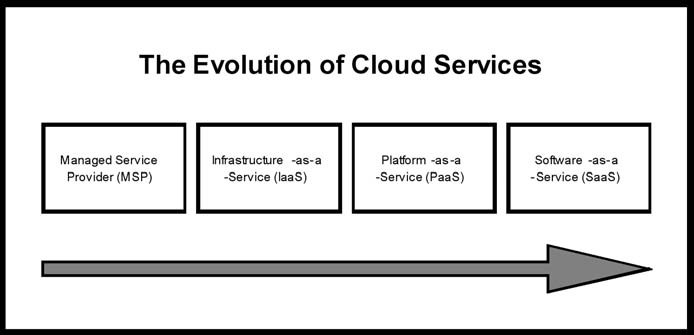
\includegraphics[scale=1]{gambar29.jpg} \\
\textbf{Gambar  2.9} Evolusi Layanan Awan. 
\end{center}
Seperti halnya dengan penyedia layanan yang diatur, perusahaan atau pengguna akhir perlu kebijakan penelitian vendor pada keamanan data sebelum menggunakan jasa vendor untuk menghindari  kehilangan atau tidak dapat mengakses data mereka.\\
Analis teknologi dan perusahaan konsultan Gartner mendaftar tujuh isu keamanan yang mana salah satu diantaranya  harus dibahas dengan perusahaan \textit{Cloud Computing} :\\
\begin{enumerate}
\item \textbf{Hak istimewa dari pengguna akses.}\\
Menanyakan tentang siapa yang memiliki akses khusus untuk data, dan tentang pengangkatan dan pengelolaan administrator tersebut.
\item \textbf{Peraturan kepatuhan.}\\
Pastikan bahwa vendor bersedia untuk menjalani audit eksternal dan / atau sertifikasi keamanan.
\item \textbf{Lokasi data.}\\
Apakah   penyedia   layanan   dalam   hal   ini   perusahaan   \textit{Cloud  Computing} melakukan pengendalian terhadap lokasi data.
\item \textbf{Pembagian / pemisahan data.}\\
Pastikan bahwa enkripsi tersedia di semua tahapan, dan bahwa skema enkripsi dirancang dan diuji  oleh para profesional berpengalaman.
\item \textbf{Pemulihanan / pembaruan.}\\
Cari tahu apa yang akan terjadi pada data sewaktu terjadi bencana / kerusakan. Mereka menawarkan pemulihan lengkap? Jika demikian, berapa lama waktu yang dibutuhkan untuk pemulihan tersebut sehingga pengguna layanan dapat menerima / mengambil data mereka sesuai kebutuhan denganmcepat dan tepat.
\item \textbf{Bantuan investigasi / bantuan penyelidikan.}\\
Apakah vendor memiliki kemampuan untuk menyelidiki setiap kegiatan  yang  tidak  patut atau ilegal?
\item \textbf{Kelayakan / kelangsungan jangka panjang.}\\
Apa yang akan terjadi pada data jika perusahaan yang bersangkutan(vendor) keluar/berhenti  dari bisnis? Bagaimana data yang dikembalikan, dan dalamformat apa?
\end{enumerate}
Menentukan jaminan keamanan data untuk jaman sekarang(hari-hari ini) begitu sulit, sehingga fungsi keamanan data menjadi begitu penting dibandingkan masa lalu. Taktik yang tidak terhandle oleh Gartner adalah meng-enkripsi data diri anda. Jika Anda mengenkripsi data menggunakan algoritma yang terpercaya, maka terlepas dari keamanan penyedia layanan dan kebijakan enkripsi, data hanya akan dapat diakses dengan kunci dekripsi.Tentu saja, ini mengarah ke tindak lanjut pada masalah: Bagaimana Anda mengelola kunci pribadi dalam infrastruktur komputasi  \textit{pay-on-demand} ?\\\\
\textbf{Masalah  keamanan data \textit{Cloud Computing.}}
\begin{enumerate}[label=\alph*]
\item \textbf{Masalah keamanan dari Virtual  machine.}\\\\
Apakah \textit{Blue Cloud} IBMatau Windows Azure di Microsoft, teknologi mesin virtual dianggap sebagai platform komputasi awan dari komponen fundamental, perbedaan antara \textit{Blue Cloud} dan Windows Azure adalah bahwa virtual mesin berjalan pada sistem operasi Linux atau sistem operasi Microsoft Windows. Teknologi virtual mesin membawa keuntungan yang nyata, ini memungkinkan pengoperasian server tidak lagi bergantung pada perangkat fisik. Tapi pada server virtual.  Pada  mesin virtual, perubahan yang fisik terjadi atau migrasi tidak  mempengaruhi layanan yang diberikan oleh penyedia layanan. jika pengguna membutuhkan jasa lebih, penyedia dapat memenuhi kebutuhan pengguna tanpa harus memperhatikan perangkat keras fisik.\\
\tab Namun, server virtual dari kelompok server logis membawa banyak masalah keamanan. Pengamanan terhadap pusat data tradisional diukur pada platformperangkat keras, sementara \textit{Cloud Computing} mungkin merupakan server dari   beberapa server virtual, server virtual mungkin milik kelompok server yang berbeda logis, server virtual, sehingga ada kemungkinan saling menyerang, yang membawa server virtual pada banyak ancaman keamanan.\\
Virtual mesin membentang pada tepi \textit{Cloud} yang membuat hilangnya batas jaringan sehingga mempengaruhi hampir semua aspek keamanan, isolasi fisik tradisional dan infrastruktur keamanan berbasis hardware tidak dapat menghentikan lingkungan komputer \textit{Cloud} yang saling menyerang antara virtual mesin.\\
\item \textbf{Keberadaan super – user.}\\\\
Untuk perusahaan yang menyediakan layanan komputasi awan (\textit{Cloud Computing}), mereka memiliki hak untuk melaksanakan pengelolaan dan pemeliharaan data, adanya super-user sangat bermanfaat untuk menyederhanakan fungsi manajemen data, tetapi merupakan  ancaman serius bagi pengguna pribadi. Dalam era privasi pribadi, data pribadi harus benar- benar dilindungi, dan fakta membuktikan bahwa \textit{platform  Cloud  Computing} memberikan layanan pribadi dalam kerahasiannya. Bukan hanya pengguna individu tetapi juga organisasi memiliki potensi ancaman serupa, misalnya pengguna korporat dan rahasia dagang disimpan dalam platform komputasi awan mungkin dicuri. Oleh karena itu penggunaan hak super user harus dikendalikan di awan(\textit{Cloud}).
\item \textbf{Konsistensi data.}\\\\
Lingkungan Awan (\textit{Cloud}) merupakan lingkungan yang dinamis, dimana data pengguna mentransmisikan data dari data center ke pengguna. Untuk sistem, data pengguna berubah sepanjang waktu. Membaca dan menulis data berkaitan dengan identitas otentikasi pengguna dan hal perijinan. Dalamsebuah mesin virtual, mungkin ada data pengguna yang berbeda 'yang harus wajib dikelola. Model  kontrol akses tradisional  dibangun di  "tepi" komputer, sehingga sangat lemah untuk mengendalikan pembaca dan penulis di antar komputer   yang terdistribusi.\\
\tab Hal ini jelas bahwa kontrol akses tradisional, jelas sangat tidak cocok untuk lingkungan komputasi awan. Dalam lingkungan komputasi awan, mekanisme kontrol akses tradisional memiliki  kekurangan serius.\\
\end{enumerate}
Prinsip keamanan data.\\\\
Semua teknik keamanan data dibangun pada kerahasiaan, integritas dan ketersediaan dari tiga prinsip dasar. Kerahasiaan mengacu pada apa yang disebut dengan data aktual atau informasi yang tersembunyi, terutama pada daerah yang sensitive, kerahasian data berada pada persyaratan yang lebih ketat. Untuk komputasi awan, data disimpan di "pusat data", keamanan dan kerahasiaan data pengguna, merupakan hal  yang penting.\\\\
Model  keamanan data.\\\\
Berikut gambar  model  keamanan data pada \textit{Cloud Computing}.\\
\begin{center}
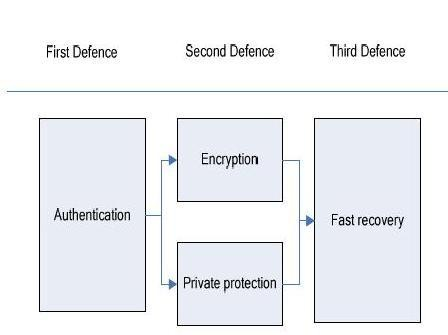
\includegraphics[scale=1]{gambar210.jpg} \\
\textbf{Gambar  2.10} Model Keamanan Data. 
\end{center}
Model struktur yang digunakan adalah system pertahanan tiga tingkat. di mana setiap tingkat melakukan tugas masing-masing untuk memastikan keamanan data dari lapisan awan(\textit{cloud}). Lapisan pertama: bertanggung jawab untuk otentikasi pengguna, pengguna  sertifikat  digital  yang diterbitkan oleh yang sesuai/berwenang, mengatur  hak akses pengguna.\\
Lapisan kedua: bertanggung jawab untuk enkripsi data pengguna, dan melindungi privasi dari pengguna melalui cara tertentu;\\
Lapisan ketiga: Data pengguna untuk pemulihan sistem yang cepat, perlindungan sistem lapisan terakhir dari data pengguna.\\\\
Kesimpulan :\\\\
Sebagai pengembangan komputasi awan, masalah keamanan telah menjadi prioritas utama. Akhirnya kami menyimpulkan teknologi komputasi awan ini sangat tepat untuk  menjaga keamanan data.
\let\cleardoublepage\clearpage
\chapter{Jenis Layanan Cloud Computing}
\date{}
\section{Jenis Layanan \textit{Cloud Computing}}
\tab Kata - kata \textit{Cloud}, merujuk kepada suatu simbol model pada dunia IT yang menggambarkan jaringan internet. Tidak semua layanan pada internet yang dapat dikategorikan sebagai cloud computing.\\
\tab Ada setidaknya beberapa persyaratan yang harus terpenuhi oleh suatu layanan berbasis internet untuk dapat diketagorikan sebagai \textit{Cloud computing} yaitu :\\
\begin{enumerate}
\item Layanan tersebut harus bersifat on demand ; kebebasan dalam memilih salah satu layanan yang disediakan oleh provider kepada pengguna dan pengguna membayarnya berdasarkan apa yang mereka gunakan.
\item Layanan bersifat elastis / scalable ; elastis suatu layanan berbasis internet harus dapat mengakomodasi dan memenuhi permintaan serta kebutuhan pengguna kapan saja
\item Layanan yang tersedia sepenuhnya dikelola oleh provider sedangkan pengguna hanya membutuhkan koneksi internet untuk menggunakan layanan tersebut.
\item Layanan tersebut harus terukur ; sumber daya cloud yang tersedia secara transparan harus dapat dioptimasi dan terukur oleh pengguna untuk menjadi acuan dalam memenuhi kebutuhan pengguna.
\end{enumerate}
\tab Berdasarkan layanan, cloud computing terbagi dalam 7 tingkatan yang biasanya digunakan oleh pengguna yaitu \textit{software as a service, utility computing, web service, platform layanan, management service provider, e-commerce, dan integrated network}.\\
\section{\textit{Software as Service}}
\tab \textit{Software as Service} merupakan evolusi lanjutan dari konsep ASP (\textit{Application Service Provider}). \textit{Software as Service} adalah istilah terhadap software atau aplikasi tertentu berbasis internet yang ditawarkan oleh provider kepada pengguna. Dalam hal ini, provider sebagai pemegang license atas software tersebut hanya memberikan service atau layanan kepada pengguna untuk menggunakannya sesuai kebutuhan pengguna dengan demikian menghilangkan kerumitan dalam hal pemeliharaan software, operasional dan support. License, maintenance, support, tingkat kenyamanan dan keamanan atas software tersebut sepenuhnya menjadi tanggung jawab dari provider.\\
\tab Kata – kata \textit{Software} merujuk kepada perangkat lunak suatu system, dimana perangkat lunak pada umumnya memiliki beragam karakteristik. Tidak semua perangkat lunak yang beredar di pasaran dapat dikategorikan sebagai \textit{SaaS}, ada beberapa karakteristik yang harus terpenuhi :\\
\begin{itemize}
\item Berbasis internet ; software harus dapat diakses dan dikelola oleh pengguna melalui media internet.
\item Software bersifat terpusat atau ter-sentral sehingga memungkinkan pengguna untuk mengaksesnya darimana dan kapan saja.
\item Memiliki fasilitas untuk meng-update atau meng-upgrade secara terpusat sehingga pengguna tidak perlu download patch atau upgrade di masing – masing komputer.
\item Aplikasi yang ditawarkan oleh provider bersifat \textit{multi tenant}
\end{itemize}
\textit{Software as Service} menawarkan beberapa keuntungan kepada pengguna dibanding dengan model aplikasi desktop:
\begin{itemize}
\item Model rancangan dan distribusi software lebih menarik dan harga terjangkau karena memungkinkan membagi satu aplikasi kepada ratusan perusahaan dan berjalan dalam lingkungan sistem biasa. Secara luas memberikan improvisasi kepada model client /server.
\item Biaya pemakaian bandwidth untuk menjaga tingkat konektivitas relatif terjangkau.
\item Mempermudah pengguna untuk melakukan migrasi aplikasi, dengan menghilangkan sisi pembayaran license software dan keharusan membayar upgrade.
\item Meningkatkan produktivitas bagi pengguna
\end{itemize}
Gambar 3.1 menjelaskan ketika provider mempublikasikan suatu layanan \textit{SaaS} di internet dan satu atau beberapa pengguna saling menggunakannya secara bersama – sama atau on demand di dalam internet
\begin{center}
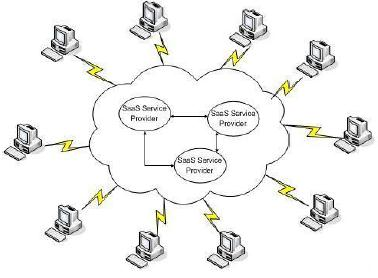
\includegraphics[scale=1]{Gambar31.jpg} \\
\textbf{Gambar 3.1}
\end{center}
\tab Implementasi \textit{cloud computing} dapat diterapkan pada jaringan yang bersifat public atau jaringan yang bersifat private. Jaringan yang bersifat public adalah suatu jaringan yang dapat diakses dan digunakan secara umum oleh setiap orang selama orang tersebut terkoneksi dengan internet sedangkan jaringan yang bersifat private adalah suatu jaringan yang hanya dapat diakses dan digunakan oleh orang – orang tertentu meskipun melalui koneksi internet.\\
\tab Ketika cloud computing diimplementasikan ke dalam jaringan public, maka seluruh sumber daya atau textit{resources} dari aplikasi sepenuhnya berada internet. Layanan textit{SaaS} yang bersifat public sering kita jumpai dalam bentuk aplikasi web atau web services. Ketika provider meletakkan seluruh sumber daya atau \textit{resources} dari aplkasi ke dalam internet tetapi hanya beberapa orang yang dapat menggunakannya maka layanan textit{SaaS} tersebut bersifat private.\\
\tab textit{SaaS} yang ditawarkan provider kepada pengguna baik melalui jaringan public maupun jaringan private pada dasarnya mempunyai satu karakteristik yang sama yaitu mudah diakses dan berskala luas (upgrade aplikasi, modifikasi aplikasi disesuaikan dengan kebutuhan dan keinginan pengguna).
\tab Berbagai textit{SaaS} yang dibuat oleh provider sering disebut dalam berbagai versi yaitu versi berbasis web, textit{on demand} dan sebagainya. Apapun versi yang dibuat oleh provider, yang diperlukan oleh pengguna adalah koneksi internet untuk dapat menggunakan textit{SaaS} tersebut.
\tab Metodologi pengembangan dari textit{SaaS} memiliki kesamaan dengan pengembangan software desktop baik dari sisi kemampuan aplikasi diakses dalam skala besar, tingkat keamanan dan aplikasi yang nyaman digunakan oleh pengguna. Beberapa faktor keberhasilan dalam implementasi dan pengembangan textit{SaaS} yaitu :\\
\begin{itemize}
\item Efisiensi sumber daya komputer : textit{SaaS} memiliki kemampuan memaksimalkan penggunaan sumber daya komputer seperti pemakaian memory dan bandwidth secara bersamaan, penggunaan database berskala besar untuk berbagai pengguna di berbagai lokasi yang berbeda dalam waktu bersamaan.
\item Optimasi data dan textit{multi tenant} : textit{SaaS} memiliki kemampuan untuk memilah data – data dan menseleksi data – data berdasarkan kepemilikan pengguna secara bersamaan dalam satu aplikasi ( textit{multi tenant} ).
\item Fleksibel aplikasi : textit{SaaS} memiliki tingkat fleksible yang tinggi dan memungkinkan pengguna memodifikasi aplikasi sesuai kebutuhan pengguna.
\end{itemize}
Berdasarkan ketiga faktor keberhasilan tersebut dan membandingkan berbagai aplikasi berbasis \textit{SaaS} yang ditawarkan oleh provider, maka kita dapat mengelompokkan berdasarkan kategori seperti yang terdapat pada gambar 3.1.1\\
\begin{center}
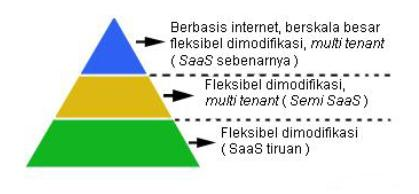
\includegraphics[scale=1]{Gambar311.jpg} \\
\textbf{Gambar 3.1.1}
\end{center}
\tab Secara arsitektur, \textit{SaaS} memiliki kesamaan dengan SOA ( textit{Service Oriented Architecture} ) yang dimiliki oleh software desktop, \textit{SaaS} memiliki dua lapisan tambahan yang tidak dimiliki oleh software desktop. Perbedaan tersebut adalah :\\
\begin{enumerate}
\item \textit{Meta data services} : lapisan ini memberikan kemudahan bagi pengguna untuk melakukan modifikasi terhadap aplikasi baik dari sisi memodifikasi tampilan aplikasi, memodifikasi fungsional aplikasi agar sesuai dengan konsep dan aturan bisnis di perusahaan pengguna, dan memodifikasi pengaturan atau kontrol terhadap data termasuk migrasi data yang tersedia. Kemudahan dalam memodifikasi aplikasi sepenuhnya di tangan pengguna.
\item \textit{Security services} : lapisan keamanan ini mendelegasikan setiap pengguna untuk bertanggung jawab sepenuhnya terhadap apapun yang dibuat di dalam aplikasi ini termasuk mendelegasikan keamanan password dari masing – masing \textit{user account ( tenant )} yang dibuat oleh pengguna. Meskipun provider sebagai pemilik sepenuhnya atas \textit{SaaS} yang ditawarkan, \textit{SaaS} memberikan kemampuan kepada pengguna untuk membuat aturan bisnis terhadap aplikasi, dan kontrol akses terhadap aplikasi sesuai keinginan pengguna.			
\end{enumerate}
Berdasarkan gambaran umum dari sisi pengguna, SaaS yang ditawarkan oleh provider terkesan sebagai satu aplikasi dalam satu database yang khusus diberikan oleh provider kepada pengguna. Gambaran umum dari sisi pengguna seperti ini tidak sepenuhnya salah karena aplikasi yang berbasis SaaS memiliki tiga model yang masing – masing model tersebut disesuaikan dengan keinginan dan kebutuhan pengguna.\\
\tab Pada gambar 3.1.2 menjelaskan tiga model berbasis SaaS yang umum ditawarkan oleh provider.\\
\begin{center}
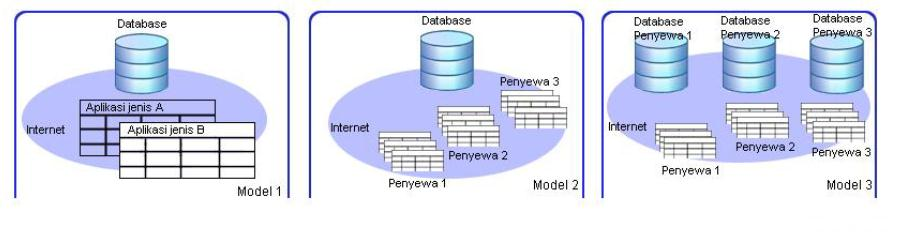
\includegraphics[scale=0.8]{Gambar312.jpg} \\
\textbf{Gambar 3.1.2}
\end{center}
Gambar 3.1.2 pada \textit{SaaS} model 1 menjelaskan pengguna atau penyewa \textit{SaaS} memiliki beberapa aplikasi yang berbeda jenis tetapi hanya memiliki satu database yang di share atau digunakan bersama – sama untuk beragam aplikasi yang dibuat oleh pengguna atau penyewa. Pengguna atau penyewa SaaS cukup melakukan modifikasi aplikasi, mengubah skala aplikasi melalui koneksi internet. \textit{SaaS} model 1 ini pada umumnya ditawarkan oleh provider dalam bentuk virtualisasi server ( VPS ) dan bersifat private.\\
\tab Pada \textit{SaaS} model 2 menjelaskan beberapa penyewa atau pengguna \textit{SaaS} memiliki aplikasi yang terpisah dan berbeda – beda tetapi mengakses database yang sama atau satu database digunakan secara bersama – sama oleh beragam aplikasi dan beragam penyewa. \textit{SaaS} model 2 ini pada umumnya ditawarkan oleh provider dalam bentuk aplikasi berbasis web atau \textit{web services}, salah satu contoh \textit{SaaS} model 2 adalah \textit{email}, terkadang demi menarik konsumen untuk menggunakan \textit{SaaS} model 2, provider memberikannya secara gratis.\\
\tab Pada SaaS model 3 menjelaskan beberapa penyewa \textit{SaaS} memiliki masing – masing aplikasi yang berbeda termasuk database yang berbeda dan bersifat private. Satu penyewa memiliki beragam aplikasi tetapi memiliki satu database private yang digunakan untuk aplikasi penyewa itu sendiri. Masing – masing penyewa terpisah secara mandiri baik dari aplikasi maupun secara database.
\textit{SaaS} model 3 ini adalah model gabungan dari model 1 dan model 2 yang memang dibangun dan dibuat oleh provider \textit{SaaS} untuk memenuhi kebutuhan pengguna. Salah satu contoh \textit{SaaS} model 3 adalah aplikasi \textit{office suite} berbasis web.\\
\tab Kesimpulan dari \textit{SaaS ( Software as a Service )} : \textit{SaaS} merupakan evolusi dari pengembangan software dimana aplikasi tersebut diletakkan di cloud atau internet. Aplikasi tersebut tersedia di internet atau cloud sehingga pengguna tidak perlu melakukan instalasi atau menjalankan aplikasi tersebut di masing – masing komputernya. Sebagai hasilnya pengguna terbebaskan dari urusan maintenance aplikasi. Oleh provider \textit{SaaS} ditawarkan sebagai \textit{pay as you use service} , artinya pembayaran atas software atau aplikasi termasuk license didalamnya tidak diperlukan, pembayaran hanya dilakukan ketika aplikasi digunakan dan biaya tersebut dihitung berdasarkan periode biasanya per bulan, per tahun.\\
\tab Untuk provider software atau yang dikenal dengan istilah \textit{software house}. \textit{SaaS} memberikan keuntungan karena aplikasi atau software yang dibuatnya terlindungi dari pembajakan software dan keuntungan dari kegunaan aplikasi yang diinginkan oleh pengguna. Pada umumnya mereka ( \textit{software house} ) meletakkan aplikasinya di dalam server berbasis cloud atau lingkungan hosting. Lingkungan hosting merupakan suatu platform yang menjadi landasan untuk aplikasi berjalan, karena itu hosting identik dengan layanan \textit{PaaS ( Platform as a service )}.\\
\tab Dari kedua sisi ini, \textit{SaaS} merupakan evolusi teknologi software yang dapat ditingkatkan menjadi \textit{multi tenant} atau banyak pengguna mengakses sumber daya yang sama. Layanan \textit{SaaS} identik dengan layanan \textit{PaaS}. \textit{PaaS} merupakan istilah dari \textit{platform as a service}, dimana pada \textit{SaaS} terfokus pada aplikasi sedangkan aplikasi itu sendiri merupakan suatu platform dan membutuhkan platform tertentu.\\
\tab Implementasi \textit{SaaS} tidak dapat berjalan dengan baik jika tidak didukung dengan infrastruktur penunjang yang solid dan baik. Dengan alasan pengembangan bisnis, jika infrastruktur penunjang sudah solid dan kuat, terkadang provider dapat menawarkannya kepada pengguna. Layanan infrastruktur ini dikenal sebagai \textit{utility computing}.\\

\section{\textit{Utility Computing}}
\tab \textit{Cloud computing} tidak hanya melibatkan sisi aplikasi atau perangkat lunak saja, tetapi juga melibatkan perangkat keras atau hardware dan sumber daya penunjang. Seperti yang telah kita ketahui layanan \textit{SaaS} lebih berfokus pada aplikasi atau perangkat lunak, sedangkan pada infrastruktur sebagai layanan \textit{utility computing}. Layanan \textit{utility computing} dikemas oleh provider dalam bentuk teknologi virtualisasi dan dikenal sebagai layanan \textit{IaaS ( Infrastructure as a Service )}. Pada gambar 3.2 menjelaskan arsitektur komputer secara traditional atau standalone.\\
\begin{center}
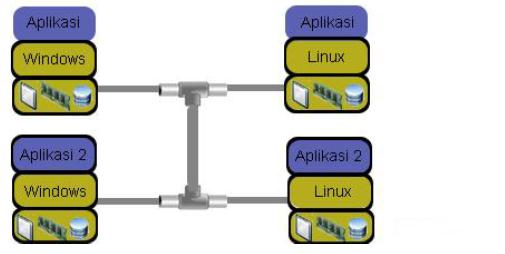
\includegraphics[scale=1]{Gambar32.jpg} \\
\textbf{Gambar 3.2}
\end{center}
\begin{center}
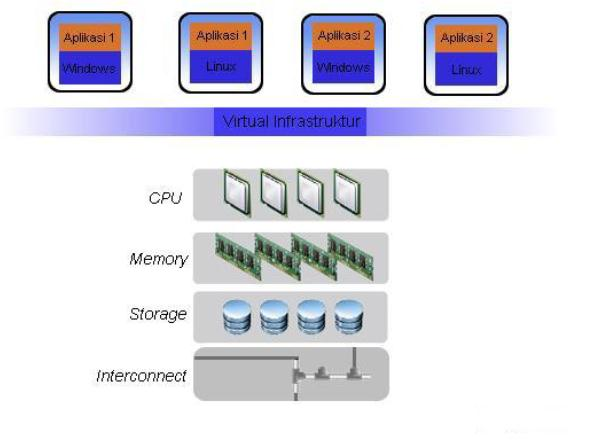
\includegraphics[scale=1]{Gambar321.jpg} \\
\textbf{Gambar 3.2.1}
\end{center}
Pada gambar 3.2.1 masing – masing aplikasi dan masing – masing sistem operasi ( windows dan linux ) menggunakan sumber daya komputer yang sama. Sistem operasi pada gambar tersebut bukanlah sesuatu yang special sebagai peranan utama dalam infrastruktur virtualisasi. Sistem operasi hanya sebagai perantara untuk dapat menjalankan virtual mesin.\\
\tab Peranan utama dalam infrastruktur virtualisasi adalah \textit{hypervisor}. \textit{Hypervisor} merupakan software yang menggantikan fungsi utama dari operating sistem ketika operating sistem selesai menjalankan virtual mesin. \textit{Hypervisor} diasumsikan sebagai \textit{virtual machine manager}, yang didesign untuk dapat menjalankan virtual mesin lainnya dan menjalankan sistem operasi dari awal seperti ketika komputer dinyalakan. Untuk lebih jelas mengenai arsitektur virtualisasi dapat dilihat pada bab 2.\\
\tab Dengan teknologi virtualisasi, pengguna atau penyewa \textit{IaaS} dapat mengakses dan menggunakan seluruh sumber daya komputer dan seluruh sumber daya lainnya yang tersedia di dalam \textit{cloud} sesuai kebutuhan dan keinginan pengguna.\\
\tab Teknologi virtualisasi memungkinkan untuk diimplementasikan berbagai aplikasi dengan tujuan yang beragam dalam 1 platform atau aplikasi, seperti \textit{storage computing, image manipulation, parallel processing, content distribution}, aplikasi web dan sebagainya. Dalam menawarkan layanan \textit{IaaS} kepada pengguna atau penyewa, provider membagi \textit{IaaS} dalam beberapa kategori layanan yaitu :\\
\begin{enumerate}
\item Layanan penyimpanan dan komputasi virtual : yaitu VMware rental, penyimpanan online ( \textit{Online Storage} ).
\item Layanan kustomise : yaitu \textit{server template}.
\item Layanan automasi dan control : yaitu \textit{automation}.
\item Layanan penghubung : yaitu \textit{remote control}, web 2.0.
\item Layanan monitoring : yaitu monitor secara fisik objek yang diinginkan ( posisi koordinat bumi, peta, kamera ).
\item Layanan optimasi objek : yaitu virtualisasi network, virtualisasi penyimpanan, virtualisasi server.
\item Layanan pengukuran objek : yaitu pengukuran fisik suatu objek.
\item Layanan integrated dan kombinasi objek : yaitu \textit{load balance}.
\item Layanan security : yaitu enkripsi data penyimpanan, VM isolation, VLAN dan SSL/SSH.		
\end{enumerate}
Jantung dari teknologi cloud computing adalah virtualisasi, dimana virtualisasi dapat diterapkan pada 2 sisi yaitu pada sisi provider dan sisi pengguna ( desktop pengguna ) seperti pada gambar 3.2.2.\\
\begin{center}
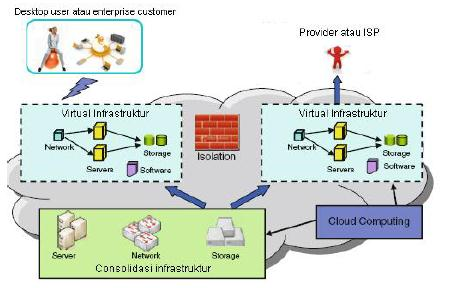
\includegraphics[scale=1]{Gambar322.jpg} \\
\textbf{Gambar 3.2.2}
\end{center}
\tab Beberapa software virtualisasi seperti VMware, citrix dan sebagainya mempunyai kemampuan untuk menciptakan fungsi lain yang disebut sebagai \textit{virtual desktop interface} ( VDI ).
\tab \textit{Virtual desktop interface} ( VDI ) menciptakan session untuk client atau user di dalam server, dan mengirimkan virtual PC tersebut kepada client atau user sehingga user dapat berinteraksi dengan server seakan client atau user tersebut berada di dalam server itu sendiri. Perbedaan yang cukup signifikan antara software remote dengan virtual PC :\\
\begin{itemize}
\item \textit{Software remote} adalah software yang dapat digunakan untuk melakukan pengendalian jarak jauh ke satu komputer atau satu server dalam satu koneksi hanya untuk satu user atau client. Jika satu komputer atau satu server diakses oleh lebih dari dua user maka komputer atau server yang diakses secara remote akan memutuskan salah satu koneksi dari dua koneksi yang terjadi.
\item \textit{Software remote} hanya software atau aplikasi penghubung ke komputer lain dan tidak dapat berfungsi untuk menciptakan komputer di dalam komputer itu sendiri.	
\end{itemize}
\tab Dalam gambar 3.2.2 user terkoneksi dan menggunakan layanan \textit{IaaS} ke server provider melalui \textit{virtual desktop interface} ( VDI ) di internet. Sedangkan pada sisi provider, provider melakukan konfigurasi server melalui jalur yang sama ( VDI ) di internet. Untuk dapat menerapkan teknologi virtualisasi di cloud maka server yang sudah diimplementasikan teknologi virtualisasi diletakkan di dalam cloud ( private cloud atau public cloud ) sebagai back end infrastruktur.\\
\tab Dari prespektif ini, sumber daya teknologi virtualisasi atau \textit{virtual resources} di dalam cloud diasumsikan sebagai sumber daya komputer yang bersifat independent atau mandiri termasuk lokasi dari sumber daya itu sendiri.\\
\tab Infrastruktur juga memegang peranan utama untuk memastikan semua komponen bekerja dengan baik dalam kondisi multi tenant dan bertanggung jawab terhadap segala aktifitas yang terjadi. Seperti yang sudah dijelaskan sebelumnya bahwa teknologi virtualisasi merupakan jantung utama dari \textit{cloud computing}, dimana teknologi virtualisasi hanyalah berupa aplikasi atau software. Teknologi virtualisasi tidak dapat berjalan sempurna tanpa didukung dengan infrastruktur yang baik dan solid. Teknologi virtualisasi memungkinkan untuk diterapkan \textit{redundancy, replication atau cluster, dan workload balancing.}\\
\begin{center}
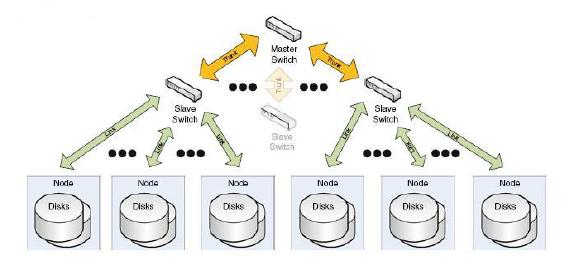
\includegraphics[scale=1]{Gambar323.jpg} \\
\textbf{Gambar 3.2.3}
\end{center}
\section{Web Service}
\tab Kemampuan unik dari \textit{web service} adalah membantu para programmer untuk membuat suatu aplikasi berbasis web dengan fungsi lain di atas platform web itu sendiri. Dalam beberapa kasus, coding – coding yang dihasilkan oleh programer yang menyewa layanan ini membagikan ( \textit{share} ) dan dikumpulkan dalam penyimpanan data yang dikelola oleh provider.\\
\tab Pada kasus lainnya, aplikasi – aplikasi tersebut dalam bentuk \textit{application programming interface} ( API ), plug-ins, atau full aplikasi yang dapat diintegrasikan dengan aplikasi berbasis web. Semua aplikasi tersebut tidak hanya tersedia hanya untuk kalangan programer yang menyewa layanan ini, tetapi juga untuk para programer pada umumnya.
\tab Pada layanan selain \textit{web service}, provider hanya bertanggung jawab untuk menjaga dan mengelola infrastruktur penunjang. Sedangkan pada layanan \textit{web service} ini, secara umum provider berusaha untuk menyediakan dan memberikan sekumpulan tools atau aplikasi penunjang yang lengkap yang dapat mempermudah para programer aplikasi web untuk membuat aplikasi. Kolaborasi dari aplikasi penunjang pada layanan ini diperoleh karena kerja sama antar partner bisnis dimana partner bisnis tersebut merupakan programmer atau institusi independent yang membangun aplikasi berbasis web.\\
\tab Bagi para programer, layanan ini merupakan pendekatan dan cara termudah dalam mendesign, dan membuat aplikasi berbasis web dengan komitmen pembayaran yang lebih murah dan terjangkau pada hardware dan software. Biaya yang dikeluarkan atas layanan ini masih terjangkau dibandingkan dengan menggunakan biaya atas jasa pembuatan aplikasi dan biaya maintenance.\\
\tab Layanan ini membantu programer untuk fokus kepada mendesign dan membuat aplikasi berbasis web. Ada dua faktor yang menentukan suatu aplikasi berbasis web dikategorikan sebagai buruk atau baik yaitu penampilan dan bobot kualitas isinya ( \textit{content} ).\\
\tab Penampilan membutuhkan keahlian dan kreatifitas dalam mendesign semua komponen, elemen serta style atau gaya design. Penampilan dari aplikasi berbasis web merupakan faktor penentu banyak orang yang berinteraksi dalam aplikasi tersebut, sedangkan content atau kualitas isinya yang mengelola informasi harus mudah dimengerti dan mudah dibaca oleh user.\\
\tab Peranan utama dari web service terletak pada \textit{application programming interfaces} ( API ) yang melekat pada \textit{web service}. Menggunakan \textit{web service} berbasis API identik dengan mengakses protocol berbasis SOAP ( \textit{Simple Object Access Protocol} ). Model pemograman API seperti mengakses dan menggunakan aplikasi di luar dari lingkungan seharusnya aplikasi tersebut berada, dimana lokasi data dan layanan protocol aplikasi tersebut berbeda lokasi.\\
\tab Karena aplikasi dengan lokasi data termasuk protocolnya terpisah dan berbeda lokasi, maka menjadi tanggung jawab programer untuk memastikan aplikasi berbasis API dapat digunakan.\\
\tab Pendekatan model pemograman API sudah digunakan dan diterapkan oleh banyak provider besar, beberapa contoh provider yang menerapkan model ini adalah google, facebook, dan Microsoft. Untuk pembahasan lebih lanjut mengenai penerapan yang dilakukan oleh provider ini dapat dilihat pada bab 4.\\
\tab Pada dasarnya web service merupakan aplikasi berbasis web yang mengkombinasikan antara data dan fungsi aplikasi dari berbagai lokasi. Aplikasi itu sendiri hanya merupakan sekumpulan kode – kode program yang diletakkan pada lokasi yang berbeda dari data dan protocol yang digunakan.\\
\tab Tiga faktor yang menjadi peranan utama dalam kesuksesan layanan web service adalah :
\begin{enumerate}
\item Menyediakan sarana berbasis aplikasi yang memungkinkan para programer untuk membangun atau membuat suatu aplikasi.
\item Menyediakan sarana bagi user atau pengguna untuk dapat menggunakan aplikasi yang memberikan efek manfaat atau kegunaan sesuai kebutuhan pengguna dan memiliki koneksitas berskala luas.
\item Menyediakan sarana bagi pengguna atau programer untuk dapat melakukan maintenance secara mandiri dan mengintegrasikan dengan aplikasi lainnya.
\end{enumerate}
Pada gambar 3.3, merupakan arsitektur dari \textit{web service}\\
\begin{center}
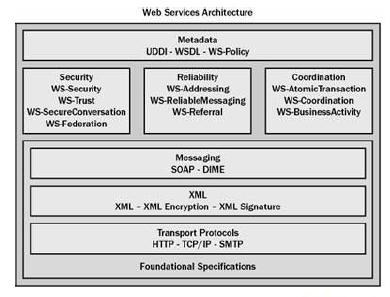
\includegraphics[scale=1]{Gambar33.jpg}\\
\textbf{Gambar 3.3}
\end{center}
\tab Seperti yang telah dibahas pada awal subbab 3.3, \textit{web service} menggunakan platform \textit{application programming interface} ( API ). Prinsip dasar dari API identik dengan SOAP ( simple object application protocol ) seperti pada gambar 3.3 didalam arsitektur web service terdapat lapisan yang disebut dengan SOAP.\\
\tab SOAP merupakan protocol yang bertanggung jawab terhadap pertukaran data atau informasi yang secara desentralisasi dan terdistribusi. Protocol yang digunakannya adalah http ( \textit{hypertext transfer protocol} ).\\
\tab Peranan SOAP di dalam teknologi \textit{web service} adalah sebagai protocol yang melakukan pemaketan pesan – pesan ( \textit{messages} ) yang digunakan secara bersama oleh aplikasi – aplikasi penggunanya. Spesifikasi pemaketannya sendiri tidak lebih dari sebuah amplop biasa berbasis XML untuk sebuah informasi yang akan dikirim, serta sekumpulan aturan bagi translasi aplikasi dan tipe – tipe data dari platform yang spesifik.\\
\tab Pesan dari SOAP adalah sebuah dokumen XML yang terdiri atas beberapa element :\\
\begin{enumerate}
\item Elemen \textit{envelope} : elemen yang mengidentifikasi dokumen XML sebagai sebuah pesan SOAP.
\item Elemen \textit{header} : elemen ini bersifat opsional, berisi informasi header.
\item Elemen \textit{body} : berisikan panggilan dan merespon informasi.
\item \textit{Fault} elemen : elemen yang bersifat opsional, berisikan pesan kesalahan yang terjadi pada waktu proses.

\end{enumerate}
Contoh bentuk dari dokumen XML seperti pada gambar 3.3.1.\\
\begin{center}
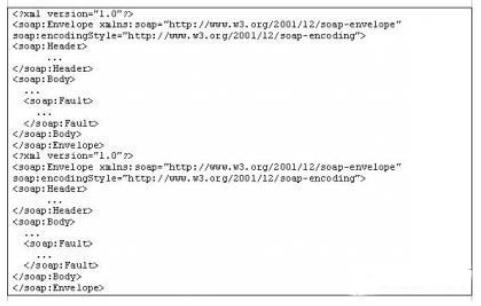
\includegraphics[scale=1]{Gambar331.jpg}\\
\textbf{Gambar 3.3.1}
\end{center}
\tab Pada gambar 3.3.2 secara umum \textit{web service} terbentuk dari semua komponen yang bersifat abstrak, bervariasi dan dinamis. Semua komponen tersebut saling terkait secara berkesinambungan dan menghasilkan suatu aplikasi yang \textit{user friendly} atau mudah digunakan bagi pengguna. Komponen – komponen tersimpan secara terpusat dalam lokasi yang dikenal sebagai portal.\\
\tab Beberapa provider seperti google, Microsoft dan facebook memperluas jangkauan layanan ini dalam berbagai device atau alat mobile untuk memperluas jangkauan penyebaran informasi.\\
\begin{center}
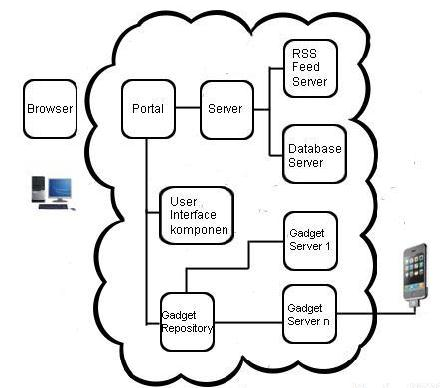
\includegraphics[scale=1]{Gambar332.jpg}\\
\textbf{Gambar 3.3.2}
\end{center}
\section{\textit{E Commerce}}
\tab Ketika aplikasi berbasis web menjadi salah satu teknologi penunjang yang menghubungi pelanggan, rekan bisnis dan karyawan kepada aplikasi perusahaan melalui jaringan internet, \textit{e commerce} berkembang pesat menjadi suatu aplikasi berbasis web yang mengakomodasi berbagai kebutuhan pelanggan.\\
\tab \textit{E commerce} yang merupakan istilah dari perdagangan berbasis elektronik mengharuskan perusahaan untuk melakukan integrasi antara sisi internal dan eksternal proses bisnis mereka kepada era teknologi dan informasi berbasis aplikasi web.\\
\tab Ketika perusahaan melibatkan proses bisnis mereka melalui jaringan intranet, extranet kemudian melalui jaringan internet, \textit{e commerce} berhasil menekan sisi biaya, menjangkau pemasaran lebih luas dan meningkatkan hubungan bisnis mereka kepada rekan bisnis.\\
\tab Seiring dengan berkembangnya \textit{e commerce}, perusahaan berhasil meraih keuntungan bisnis, salah satu contoh perusahaan yang berhasil meraih keuntungan terbesar melalui \textit{e commerce} adalah Amazon.com.\\
\tab Bagaimanapun juga keberhasilan yang diraih oleh \textit{e commerce} melalui jaringan internet memiliki beberapa resiko finansial dalam bertransaksi. Atas dasar ini subbab dari 3.4 lebih terfokus pada sisi arsitektur dari provider keamanan transaksi dan sisi skalabilitas aplikasi web.\\
\tab Melihat pada resiko keamanan secara finansial dalam bertransaksi \textit{e commerce}, banyak industri atau perusahaan yang meng-integrasikan aplikasi berbasis web mereka dengan provider keamanan transaksi atau perusahaan yang berfokus pada keamanan transaksi.\\
\tab Untuk mempermudah dalam memahami sisi arsitektur dan skalabilitas aplikasi web untuk diintegrasikan dengan provider keamanan transaksi, maka diambil salah satu contoh provider security ( keamanan transaksi ) yaitu paypal.\\
\tab Seperti yang telah dibahas arsitektur aplikasi berbasis web pada subbab 3.3, arsitektur dari paypal adalah \textit{web service} atau aplikasi web berbasis SOAP (\textit{ simple object access protocol }), yang memberikan skalabilitas untuk mengintegrasikan dan mengkombinasikan \textit{client side} dan \textit{server side}.
\begin{center}
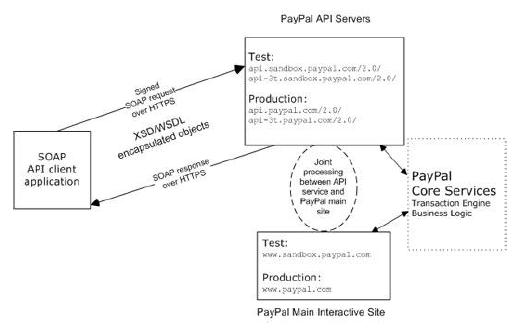
\includegraphics[scale=1]{Gambar34.jpg}\\
\textbf{Gambar 3.4}
\end{center}
\tab Pada gambar 3.4 dalam model OOP ( \textit{object oriented programming} ) ini, interface ke SOAP request/response merupakan objek dari bahasa pemograman native yang dapat diintegrasikan ke SOAP dari aplikasi web. Paypal menyediakan file – file WSDL dan XSD yang secara spesifik merupakan struktur message atau pesan dari paypal, isi data, dan layanan ( service ) API dari paypal.\\
\tab Aplikasi bisnis termasuk data didalamnya berada dan berjalan dalam property objek ini. Untuk mengirim dan menerima data dapat dilakukan dengan metode pemanggilan objek tersebut. Objek SOAP client menangani permintaan membentuk SOAP baru dan mengirimkan kepada layanan paypal, kemudian layanan paypal memberikan umpan balik atau \textit{feedback} ke objek SOAP client.\\
\tab Skema dan prinsip dasar dari web service paypal adalah \textit{eBay business language} ( eBL ). Dan inti komponen yang diperlukan dalam mengintegrasikan aplikasi web ke layanan paypal adalah API paypal yaitu file – file WSDL dan XSD.\\
\tab Secara mendasar konsep dan terminology dari API paypal adalah :\\
\begin{itemize}
\item \textit{API calls} : Layanan API paypal, melalui fungsi objek ini, perusahaan bisnis atau organisasi dapat melakukan pembayaran via online, pencarian transaksi, pengembalian ( refund ) pembayaran, melihat informasi transaksi dan beberapa fungsi lain yang diperlukan oleh dunia bisnis.
\item \textit{API certificate} : Merupakan \textit{API signature}, paypal akan memberikan satu digital sertifikat yang bersifat unik yang dapat didownload dari website paypal. Fungsi ini akan digunakan oleh setiap komputer user yang akan mengakses, dan sertifikat ini akan me-\textit{encrypt} data ketika objek \textit{API calls} dipanggil atau digunakan melalui protocol https dan mengirimnya ke API server.
API sertifikat ini sangat cocok diterapkan ke \textit{web server}.
\item \textit{API signature} : Merupakan \textit{API certificate}, paypal akan memberikan satu \textit{digital signature} ( satu baris dari text atau metode pengacakkan hash ) yang dapat diperoleh dengan mengcopy \textit{API calls} nya. Sebagai fungsi alternative dari \textit{API certificate}.
\textit{Digital signature, API username}, dan \textit{API password} semuanya merupakan bagian yang disebut sebagai tiga token \textit{authentication}.
\item \textit{API username }dan
\textit{API password} : Di \textit{generate} atau dibuat oleh paypal, yang meidentifikasikan nama rekening dan password yang secara special digunakan untuk \textit{API calls}.
Selalu melibatkan username dan password setiap kali menggunakan dan memanggil\textit{ API call.}
\textit{API username }dan \textit{API password} berbeda dengan penggunaan ketika login ke website paypal. Pada website paypal, untuk login yang diperlukan adalah email dan password yang berbeda dari \textit{API username} dan \textit{API password.}
\item \textit{Subject authorization} : Sebagai indikator bagi \textit{API call}, yang merupakan informasi rekening \textit{API call} itu dibuat.
Ini merupakan aspek yang dibuat oleh provider paypal sebagai authorisasi.
\item \textit{First-party access} : Perusahaan atau organisasi diberikan kebebasan untuk membuat \textit{API call} dari server miliknya ke server paypal.
Perusahaan diperbolehkan untuk memiliki \textit{API certificate }atau \textit{API signature, username} dan \textit{password} sebagai miliknya.
Sebagai contoh :
Programer dari perusahaan \textit{merchant}, memperoleh file \textit{API certificate} yang diterbitkan oleh paypal. Oleh programmer tersebut dibuatkan \textit{API call} untuk perusahaannya dari server milik perusahaannya.
\end{itemize}
Pada gambar 3.4.1 merupakan diagram dari \textit{SOAP request.}
\begin{center}
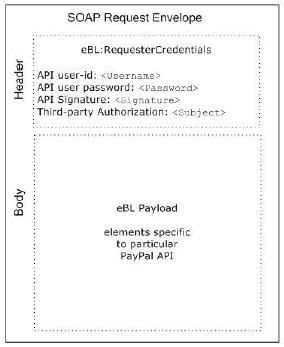
\includegraphics[scale=1]{Gambar341.jpg} \\
\textbf{Gambar 3.4.1}
\end{center}
\tab Kesimpulan dari \textit{ecommerce} : pondasi dari \textit{ecommerce} adalah tekonologi \textit{web service} yang memiliki skalabilitas untuk diintegrasikan dengan aplikasi lain yang berbeda lokasi dan berbeda provider. Karena \textit{e commerce} merupakan \textit{web service} yang terfokus pada bisnis, maka secara implisit \textit{e commerce} memiliki resiko keamanan dalam bertransaksi.\\
\tab Melihat dari resiko keamanan secara finansial, banyak perusahaan bisnis menyerahkan tanggung jawab keamanan bertransaksi online kepada provider lain yang fokus kepada keamanan transaksi. Salah satu arsitektur dari provider yang dibahas adalah paypal.\\
\tab \textit{E commerce} berbasis \textit{web service} memiliki kesamaan arsitektur dengan arsitektur yang dimiliki \textit{provider security} ( paypal ) yaitu API atau \textit{application programming language} sehingga memiliki kemampuan untuk diintegrasikan ke aplikasi milik provider paypal.\\
\tab Ketika \textit{provider security} ( keamanan transaksi ) seperti paypal terintegrasi melalui internet dengan banyak aplikasi \textit{e commerce} dari berbagai perusahaan bisnis (\textit{ multi tenant} ) maka dapat dikatakan \textit{e commerce} tersebut berbasis \textit{cloud computing}.
Provider paypal tidak hanya menawarkan layanan \textit{security} ( keamanan bertransaksi ) secara online melalui aplikasi web tetapi juga menyediakan \textit{plug ins} untuk \textit{payment online} berbasis aplikasi.\\

\section{\textit{Management Service Process}}
Seperti yang telah dibahas, cloud computing memiliki beberapa layanan seperti pada gambar 3.5.
\begin{center}
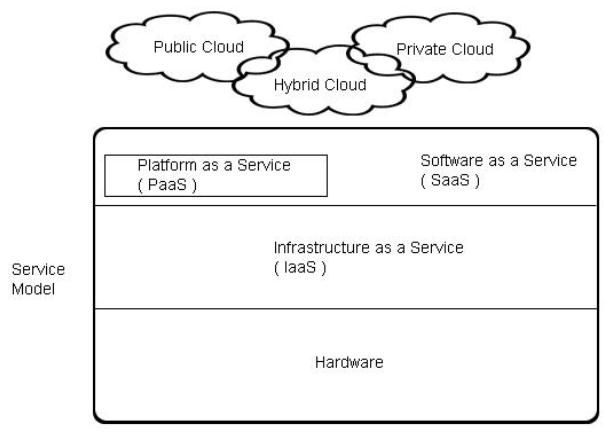
\includegraphics[scale=1]{Gambar35.jpg}\\
\textbf{Gambar 3.5}
\end{center}
\tab \textit{Cloud computing} memberikan banyak keuntungan yang secara umum yaitu dapat ditingkatkan skala pengembangan, dapat dihandalkan, dan keamanan. Sedangkan bagi pengguna memberikan kemudahan dan keuntungan dalam menekan biaya baik dari sisi IT maupun dari sisi operasional.\\
\tab Sedangkan bagi provider memberikan kemudahan bagi pengelolaan, menekan biaya dalam maintenance layanan, memberikan kemudahan dalam melakukan diffrensiasi produk dengan penggunaan SLA, optimasi resource, harga produk atau service yang dijual lebih terjangkau.\\
\tab Karena setiap layanan yang terdapat pada cloud terkait dengan pelayanan public dan bisnis serta teknologi informasi yang menjadi peranan utama ( IT ), maka organisasi ICT ( \textit{information and communication technologies} ) membuat standarisasi yang mengatur pelayanan cloud computing yaitu ITIL V3 dan ISO/IEC 20000 : 2005.\\
\tab Berikut ini adalah beberapa tolak ukur yang digunakan untuk menilai setiap layanan yang diberikan oleh provider cloud berdasarkan ITIL V3 dan ISO/IEC 20000 : 2005\\
\begin{itemize}
\item Konfigurasi manajemen database ( CMDB ) : Pengukuran dilakukan dari sistem database yaitu, Tipe dari database, aplikasi penunjang untuk dapat memodifikasi data dalam database, backup database, relasi atar database tersebut, integrasi database dengan tipe database lain dan mendapatkan bantuan teknis dalam melakukan konfigurasi database.\\
\item \textit{Service level management} : Pengukuran dilakukan dari secara implisit terhadap setiap level dari layanan yang diberikan oleh provider dan pengukuran dimulai dari \textit{SLA ( Service Level Agreement )} yang diberikan oleh provider \textit{service cloud}.
\item \textit{Service continutity} dan \textit{availability management} : Pengukuran dilakukan dari kemudahan dan fleksiblenya layanan yang diberikan oleh provider, baik dari sisi upgrade atau downgrade layanan, dan seberapa lama layanan tersebut sudah dipublikasi dan dijual ke pasaran.
\item \textit{Resolution process} : Pengukuran dilakukan dari kemampuan team manajemen provider dalam menangani berbagai proses seperti \textit{indicents} ( bencana ), \textit{problem technical} ( masalah teknis ) dan tanggapan atas permintaan tertentu atau perubahan tertentu.
\item \textit{Service reporting} : Pengukuran dilakukan dari kemampuan provider dalam menyediakan laporan baik terhadap layanan yang digunakan, laporan historical layanan tersebut digunakan, laporan waktu penggunaan layanan yang dibeli.
\item \textit{Capacity management} : Pengukuran dilakukan atas performance provider baik dari sisi teknis maupun sisi manajemen. Pengukuran ini menghasilkan nilai kemampuan provider dalam memenuhi setiap kebutuhan konsumennya.
\item \textit{Information security management} : Pengukuran dilakukan dari sisi keamanan sistem, jaringan atau network yang tersedia, dan sisi keamanan infrastruktur yang dimiliki oleh provider. Bahkan pengukuran ini dilakukan dari sisi teknologi keamanan data yang dimiliki oleh provider.
\item \textit{Business relationship management} : Pengukuran diukur dari beberapa faktor bisnis yang akhirnya akan memberikan hasil kemampuan provider dalam menfasilitasi dan menyediakan solusi bagi bisnis.
\end{itemize}
Dari beberapa pengukuran seperti yang dijelaskan diatas, maka dapat dikelompokkan dalam beberapa kategori yang dapat diukur :\\
\begin{itemize}
\item \textit{Incident} manajemen : kata \textit{incident} memiliki arti sesuatu hal yang tidak diinginkan dan terjadi dalam waktu yang tidak direncanakan. Konotasi dari \textit{incident} lebih memiliki nuansa negatif. \textit{Incident} manajemen adalah sebuah proses untuk mengatasi dan menangani segala kejadian buruk yang mungkin terjadi, termasuk masalah teknis dan pertanyaan yang diberikan oleh pengguna.\\
Penilaiannya termasuk:
\begin{itemize}
\item Kemampuan untuk mendeteksi dan mengatasi setiap kejadian. Hasilnya berupa nilai / presentasi \textit{downtime}.
\item Kemampuan untuk mengidentifikasi prioritas bisnis secara \textit{realtime} dan pengalokasian sumber daya komputer secara dinamis.
\item Kemampuan untuk mengidentifikasi potensi kejadian yang mungkin terjadi. Hasilnya berupa opini atau rekomendasi solusi.
\item Kemampuan \textit{helpdesk} dalam mengatasi keluhan dan masalah.
\end{itemize}
\item \textit{Change} manajemen : Memastikan setiap perubahan yang terjadi sepengetahuan pengguna, mendapatkan persetujuan, dan dikaji ulang kembali sebelum diimplementasikan oleh pengguna. \textit{Change} manajemen memastikan setiap perubahan yang terjadi dalam pengendalian pengguna. Dapat dilihat pada gambar 3.5.1
\begin{center}
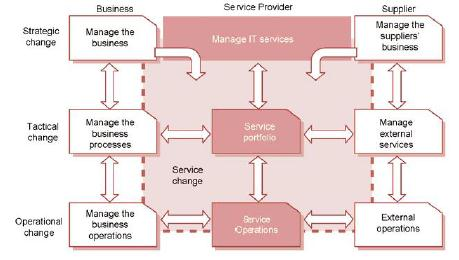
\includegraphics[scale=1]{Gambar351.jpg}\\ 
\textbf{Gambar 3.5.1}
\end{center}
\item \textit{Capacity} manajemen : Memastikan biaya yang dikeluarkan sesuai dan seimbang dengan ukuran atau harapan yang ingin dicapai melalui investasi TI. Pengukuran dilakukan dengan melihat 2 sisi yaitu :
\begin{itemize}
\item Sisi kapasitas bisnis : perencanaan dan kebutuhan bisnis diselaraskan dengan perencanaan TI di kemudian hari. Pengukuran dapat diambil dari beberapa data yang tersedia, layanan TI yang sudah tersedia, dan \textit{forecast} TI. Semua pengukuran tersebut pada dasarnya hanyalah sebuah strategi
\item Sisi kapasitas dalam pelayanan : terfokus pada pelayanan dan pengukuran performance TI yang sedang digunakan, performance operational \textit{helpdesk} TI.
\item Sisi komponen TI : terfokus pada pengendalian, utility, dan performance komponen TI. Dapat dilihat pada gambar 3.5.2.
\begin{center}
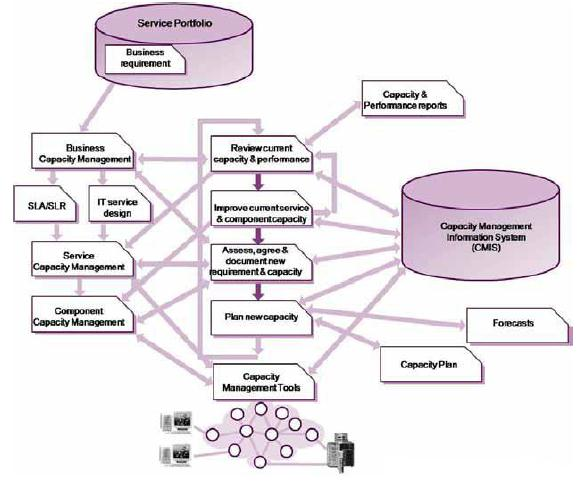
\includegraphics[scale=1]{Gambar352.jpg}\\ 
\textbf{Gambar 3.5.2}
\end{center}
\end{itemize}
\item \textit{Availability} manajemen : Terfokus pada kemampuan manajemen dalam memberikan layanan sesuai dengan kebutuhan dan keinginan pengguna. Dapat dilihat pada gambar 3.5.3
\begin{center}
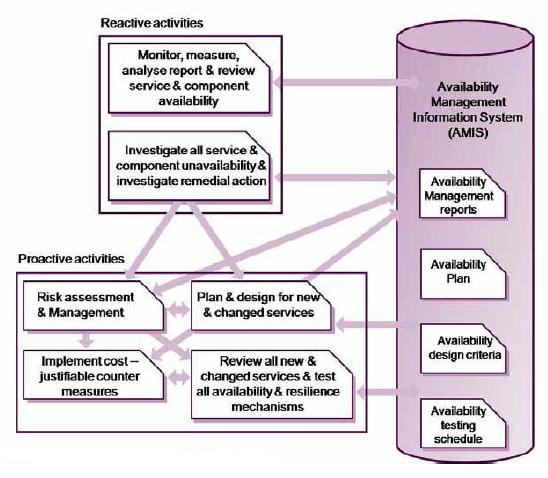
\includegraphics[scale=1]{Gambar353.jpg}\\
\textbf{Gambar 3.5.3}
\end{center}
\item \textit{Problem} manajemen : Terfokus pada usaha untuk meminimalkan akibat dari setiap kejadian, yang akan memberikan hasil kecilnya resiko yang akan ditanggung oleh bisnis. Problem manajemen terkait dengan \textit{change} manajemen setiap kali terjadi perubahan. Dapat dilihat pada gambar 3.5.4.
\begin{center}
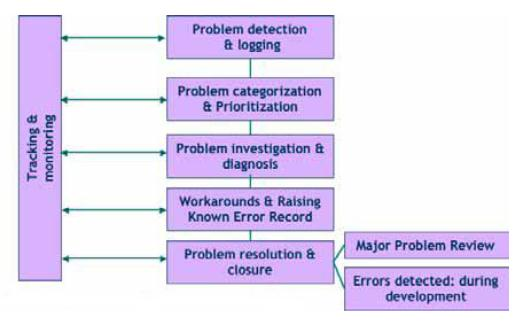
\includegraphics[scale=1]{Gambar354.jpg}\\
\textbf{Gambar 3.5.4}
\end{center}
\textit{Problem} manajemen memiliki beberapa kategori yaitu :
\begin{itemize}
\item \textit{Problem} : Sesuatu kejadian yang belum jelas, biasanya masih dalam tahap investigasi.
\item \textit{Know error} : Sesuatu kejadian yang diketahui penyebabnya, biasanya ini dilakukan setelah selesai mendiagnosis suatu masalah atau \textit{problem}.
\item KEDB : Penyebab error-nya database.
\item \textit{Workaround} : Dokumen teknis yang menjadi acuan user dalam bertindak ketika terjadi masalah.
\end{itemize}
\item \textit{Event} manajemen : Terfokus pada monitoring operasional dan pengendalian
\item \textit{Service} validasi dan \textit{testing} : Memiliki beberapa focus yang ingin diraih, yaitu:
\begin{enumerate}
\item Meningkatkan kepercayaan untuk membuat layanan baru atau mengubah layanan tertentu, meningkatkan nilai jual.
\item Menjadi validasi bahwa service atau layanan sesuai dengan kebutuhan dan keinginan pengguna.
\item Menjamin layanan sesuai dengan kebutuhan dengan menerbitkan \textit{terms and conditions use}.
\end{enumerate}
\end{itemize}
\tab Dari semua faktor pengukuran yang telah diuraikan dan mengacu kepada ITIL V3 dan ISO/IEC 20000:2005, beberapa provider memberikan jasa penilaian terhadap layanan dari provider \textit{cloud} yang lain.\\
\tab Kesimpulan dari \textit{management service process} ( MSP ) : provider cloud tertentu atau \textit{consultant cloud} memberikan jasa penilaian terhadap layanan \textit{cloud computing} yang tersedia di pasaran yang nantinya diselaraskan dengan kebutuhan dan keinginan pengguna atau bisnis, sehingga dengan jasa dari \textit{consultant cloud} ini akan didapatkan hasil layanan \textit{cloud} terbaik yang cocok untuk diimplementasikan dan mendukung kinerja dan produktifitas bisnis.\\
\tab Penilaian yang diberikan oleh \textit{consultant cloud} tentunya mengacu dan berorientasi kepada acuan dari ITIL V3 dan ISO/IEC 20000:2005\\\\
\section{\textit{Integrated Network}}
\tab \textit{Network} atau jaringan merupakan link utama atau jaringan utama yang menghubungkan antara pengguna layanan \textit{cloud} dengan penyedia pusat data dan provider layanan \textit{cloud}. Pada \textit{cloud computing} secara \textit{network} atau jaringan terbagi dalam tiga kategori :\\
\begin{enumerate}
\item \textit{Public Cloud}\\
Suatu model dari layanan \textit{cloud} yang mendeskripsikan layanan \textit{cloud} tersebut menggunakan sumber daya komputerisasi yang ditujukan, didesign dan dapat digunakan secara massal, seperti CPU atau kapasitas penyimpanan dan aplikasi atau software yang tersedia di internet.\\
Banyak provider \textit{cloud} yang menawarkan layanan berbasis \textit{cloud computing} seperti amazon EC2, force.com, google dan provider lainnya.\\
\item \textit{Private Cloud}\\
Suatu model dari layanan \textit{cloud} yang bertolak belakang dengan model \textit{public cloud}, pada model ini lebih terfokus pada kalangan tertentu dan bersifat \textit{private} atau tertutup. Biasanya layanan ini berskala \textit{enterprise}.\\
\textit{Private cloud} juga merupakan model yang merepresentasikan suatu model layanan \textit{cloud} yang bekerja di belakang jaringan atau \textit{network} perusahaan atau kepentingan pribadi user.\\
Ciri khas dari \textit{private cloud} biasanya berupa keharusan untuk membeli atau membayar layanan \textit{cloud} sebelum mencobanya. Ciri khas seperti ini menunjukkan seakan \textit{private cloud} tidak memiliki keunggulan dibandingkan dengan model \textit{cloud} yang lain.\\
Jika dilihat dari kacamata perdagangan, model \textit{private cloud }seakan menjebak konsumen atau sedikit memaksakan konsumen untuk membayar layanan \textit{cloud} tersebut sebelum menggunakannya.\\
Keunggulan dari model \textit{private cloud} adalah model layanan \textit{cloud} yang mendapatkan prioritas dalam pengembangan ( terdepan dalam inovasi ), dan lebih difokuskan kepada kalangan bisnis.\\
\item \textit{Hybrid Cloud}\\
Model yang merepresentasikan campuran antara model \textit{public cloud} dengan model \textit{private cloud}. Model \textit{hybrid cloud} ini merupakan model pengembangan dari layanan \textit{cloud} dimana provider layanan \textit{cloud} mengelola dan menggunakan internal sumber daya komputerisasinya dan menggunakan sumber daya komputerisasi dari provider \textit{cloud} yang lainnya. \\
\end{enumerate}
\textit{Hybrid cloud} memegang peranan utama dalam evolusi generasi baru paradima TI. Pada gambar 3.6 merupakan arsitektur \textit{network} dari \textit{hybrid cloud}.
\begin{center}
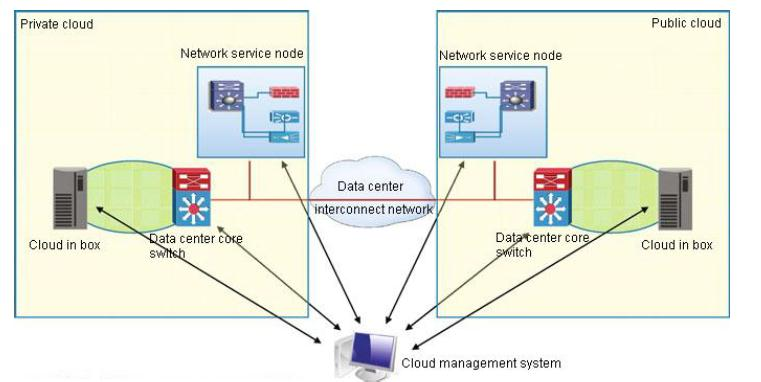
\includegraphics[scale=1]{Gambar36.jpg}\\
\textbf{Gambar 3.6 Arsitektur Network untuk \textit{Hybrid Cloud}}
\end{center}
Gambar 3.6 menjelaskan beberapa komponen utama \textit{network} membentuk suatu jaringan\textit{ private cloud} dan \textit{public cloud}, melalui jaringan \textit{interconnect} maka terjadi penggabungan dua jaringan \textit{cloud} yang berbeda menjadi satu jaringan yang disebut sebagai \textit{hybrid cloud}.\\
\tab Komponen \textit{cloud in box }adalah komponen yang diistilahkan sebagai sel nya \textit{cloud} ( \textit{cloud cell }) berfungsi sebagai \textit{pre-integrated, pre-package} dan secara aktif mengirimkan \textit{service platform} sehingga mudah dan cepat digunakan untuk diimplementasikan dalam jaringan \textit{private} dan \textit{public cloud}.\\
\tab Bentuk fisiknya, berupa \textit{chasis} tunggal layaknya server tetapi memiliki banyak \textit{slot blades ( multiple blades )}, dalam \textit{blade} terdapat beberapa unit komponen komputerisasi, beberapa storage, beberapa processor. \textit{Multiple blade} inilah yang berfungsi untuk \textit{interconnect} semua kombinasi \textit{blade} pada \textit{backplane} dan menyatukan semua koneksi \textit{Ethernet} berkecepatan tinggi ( \textit{high speed} ) yang biasanya berkecepatan 10 gigabyte \textit{fiber optic over Ethernet.}\\
\tab \textit{Core} utama dari software berbasis virtualisasi yaitu \textit{hypervisor}, secara tipikal memiliki kemampuan untuk mengembangkan lingkungan sistemnya melintasi beberapa unit komputerisasi, beberapa unit jaringan atau \textit{networking}, dan beberapa unit \textit{storage} dalam \textit{cloud-in-box}.\\
\tab Dari prespektif \textit{network}, membutuhkan \textit{virtual network switch} yang sudah di-\textit{embeded} ( sudah ditanamkan ) dalam \textit{hypervisor}, seperti yang terlihat pada gambar 3.6.1, sedangkan pada gambar 3.6.2 adalah \textit{ethernet frame} dari \textit{virtual network switch}.\\
\begin{center}
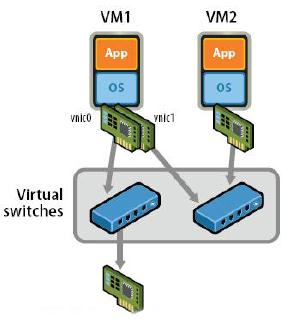
\includegraphics[scale=1]{Gambar361.jpg}\\
\textbf{Gambar 3.6.1 \textit{Virtual Network Switch}}
\end{center}
\begin{center}
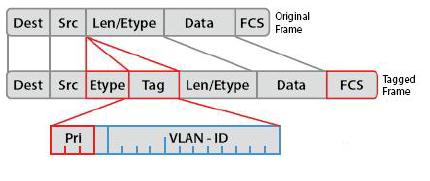
\includegraphics[scale=1]{Gambar362.jpg}\\
\textbf{Gambar 3.6.2}
\end{center}
\tab Komponen \textit{network service node} memegang peranan utama dalam arsitektur \textit{network} dari \textit{hybrid cloud, firewall} pada lapisan ini menjamin keamanan data dalam pengiriman ( \textit{secure transport} ), sedangkan \textit{load balance} pada lapisan ini berfungsi menjaga keseimbangan beban kerja yang terjadi.\\
\tab Manajemen dari \textit{network} arsitektur pada \textit{hybrid cloud} terletak pada \textit{cloud management system}. \textit{Virtual switch} memiliki kemampuan untuk mengimplementasikan aturan keamanan ( \textit{security policies }) ke dalam virtual mesin.\\
\begin{center}
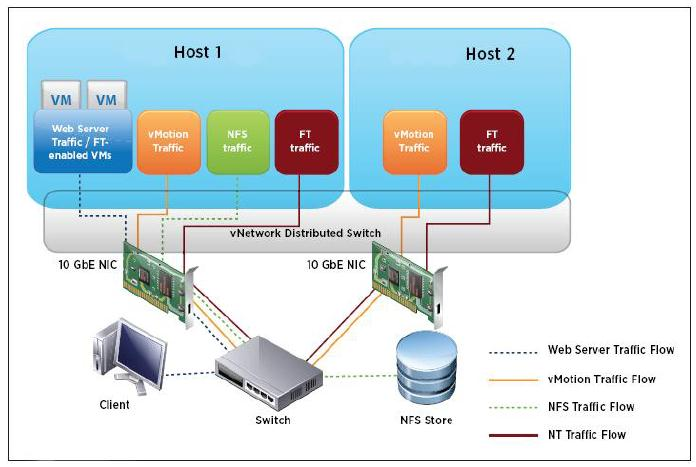
\includegraphics[scale=1]{Gambar363.jpg}\\ 
\textbf{Gambar 3.6.3 \textit{Traffic}}
\end{center}
\tab Pada gambar 3.6.3 menjelaskan aliran \textit{traffic} yang dapat dilakukan oleh \textit{virtual switch}, dimana oleh \textit{vnetwork distributed switch} atau virtual distribusi switch berperan sebagai pengendalian \textit{traffic} dan melakukan pemisahan \textit{traffic} berdasarkan alamat tujuan host.\\
\tab Atas dasar kemampuan dari \textit{vnetwork distributed switch}, maka pemakaian bandwidth menjadi efisien. Gambar 3.6.4 menunjukkan penerapan virtual mesin menggunakan bandwidth yang efisien dalam pemrosesan.\\
\begin{center}
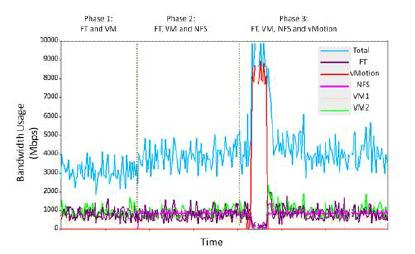
\includegraphics[scale=1]{Gambar364.jpg}\\\textbf{Gambar 3.6.4}
\end{center}
Dengan arsitektur dan kemampuan teknologi virtualisasi, provider cloud menawarkan layanan integrated network kepada pengguna dalam berbagai produk atau layanan :
\begin{itemize}
\item Untuk pengguna ( user ) : \textit{Online storage} atau CloudNAS, VPS ( \textit{virtual private server} )
\item Untuk bisnis : \textit{integrated network, MobileMe iDisk, parallel processing system, automation system, GPS}
\end{itemize}
\let\cleardoublepage\clearpage
\chapter{Penerapan Cloud Computing}
\section{Data Center Telkom}
\tab Teknologi cloud computing di Indonesia telah berjalan, dimana PT. Telekomunikasi Indonesia atau PT. Telkom telah bekerja sama dengan Microsoft dalam hal teknologi cloud computing. Layanan ini dapat membuat perusahaan dengan cepat dan mudah meningkatkan kapasitas penyimpanan, karena didapat secara virtual. Solusi yang dikembangkan oleh PT.Telkom dan Microsoft hadir dalam bentuk Microsoft Windows Exchange dan Office Communications Server Hosted dimana merupakan salah satu jalan untuk membantu bisnis di Indonesia mengadopsi teknologi cloud computing dengan biaya relatif murah. Pihak Microsoft dan PT. Telkom sepakat untuk mengembangkan bisnis cloud  computing  mulai  dari Infrastructure as a Service (IAAS), Platforms as a Service (PAAS) dan Software as a Service (SAAS) yang dikirimmelalui cloud yang aman.\\
Layanan ini mampu memberikan solusi komprehensif bagi bisnis dan insdustri  serta memberikan percepatan dalamnegeri ini pada era teknologi  cloud computing.\\
Ada  beberapa  paket  yang  ditawarkan  oleh  PT.  Telkom  dengan  teknologi   cloud  computing
diantaranya:
\begin{enumerate}
\item Paket Communication dan  Collaboration.\\
Broadband + Exchange + OCS, sebuah bentuk SaaS yang memberikan fitur teknologi microsoft united communication tanpa harus di install. Hosted OCS menawarkan  :  instant messaging dan presence, email dan united messaging, peer-to-peer voice dan video, desktop sharing di microsoft office, communication 207 R2, web-based IM, email, presence dan desktop sharing.
\item Paket  Virtualized Server\\
Broadband + virtual Dedicated Server, sebuah bentuk IaaS. Teknologi VPS (Virtual Private Servers), memungkinkan sebuah perusahaan dapat berbagi  biaya  server dengan pelanggan yang lain dengan tetap memegang kendali penuh terhadap aplikasi mereka. VPS berjalan pada web server dan memberikan akses dengan privasi  penuh dan bandwidth yang terjamin, CPU dan ruang disk.
\end{enumerate}
Pada dasarnya telkom memberikan sistem online data dimana solusi untuk sebuah perusahaan untuk mengelola data, khususnya data konsumen atau calon konsumen, teknologi ini memberikan layanan pengadaan yang bisa memberikan sistem data dan teknologi yang saling terintergrasi, reliable dan update.\\
Pada layanan ini akan dikombinasikan keseluruhan layanan yang diberikan. Produk ini dapat menjamin kegiatan bisnis yang menjamin status data selalu terupdate sepanjang tahun. Dipadu dengan kemampuan SDM yang berpengalaman dalam pengelolaan database, juga system dan data-data yang selalu terjaga dalam kondisi optimal sehingga dapat digunakan untuk berbagai kebutuhan. Hal tersebut diintegrasikan dengan kompetensi utama lainnya dari PT. Infomedia Nusantara yaitu berupa Contact Center Solutions yang dapat memberikan berbagai alternative pengadaan proses inbound/outbound call perusahaan dan juga dengan layanan Produk Konten Infomedia, yang dapat memberikan solusi lain dalam hal pengakuisisian kelengkapan data bagi kebutuhan perusahaan dan layanan outbound service berupa sms dan direct mail.\\
\begin{center}
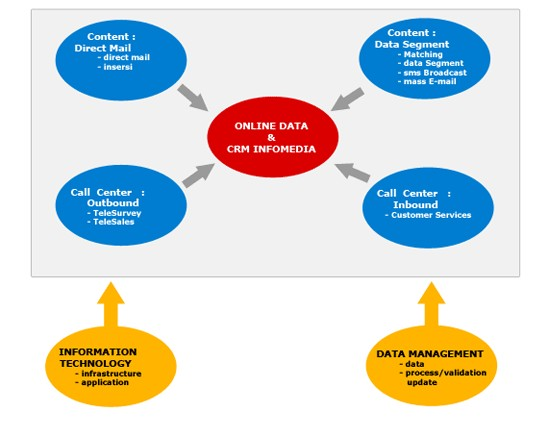
\includegraphics[scale=1]{gambar411.jpg}\\
Gambar 4.1.1  Arsitektur online data
\end{center} 
Layanan ini disediakan dengan menggunakan system online yang mana menghubungkan system data yang digunakan khusus bagi pelanggan dengan database yang terdapat di Infomedia. Dengan data processing system yang online, maka akan memberi kemudahan kepada customer untuk dapat menerima data-data sesuai dengan kondisi data yang ada di Infomedia.\\
\begin{center}
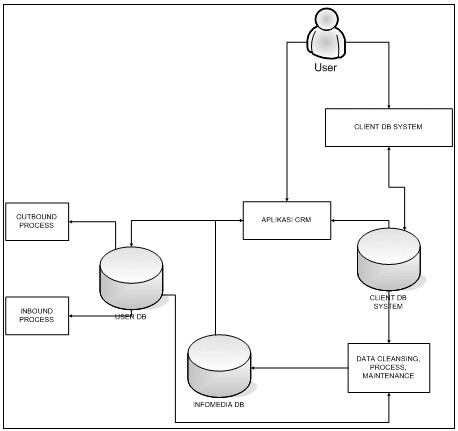
\includegraphics[scale=1]{gambar412.jpg}\\
Gambar 4.1.2  Sistem online data
\end{center}
Tujuh alasan utama menggunakan sistem secara online dimana sistem tersebut  di implementasi kan di sekolahan oleh pihak Telkom,  diantaranya :
\begin{enumerate}
\item Sistemnya serba Online dan Real-Time dapat diakses setiap saat dari mana saja\\
SIAP Online dibangun 100\% berbasis teknologi web versi 2.0 untuk dapat  diakses secara online 24 jam setiap saat dan dan dari mana saja selama Anda memiliki koneksi ke Internet. Setiap ada pengubahan data secara online, sistem SIAP Online akan memprosesnya secara langsung dalam waktu nyata (real time) untuk menjamin kenyamanan dan kesahihan setiap pengubahan (edit) data yang Anda lakukan.
\item Biaya terjangkau dan minim investasi/modal\\
Layanan SIAP Online tidak memerlukan lisensi perangkat lunak (licenced software) khusus sebagaimana produk lainnya. Anda juga tidak memerlukan investasi/modal perangkat server khusus yang terpasang lokal di sekolah atau dinas untuk mengoperasikan sistem SIAP Online. Yang Anda perlukan hanyalah sebuah web  browser di PC/ Laptop Anda yang terkoneksi ke Internet.\\
Semua perangkat utama seperti: server-server, sistem aplikasi, backup data, keamanan data hingga pemeliharaan sistemnya merupakan tanggung jawab TELKOM sebagai penyedia layanan. Dengan demikian layanan SIAP Online akan menurunkan total  biaya penggunaannya untuk Anda, institusi Anda (sekolah dan dinas). Institusi Anda juga tidak perlu melakukan investasi/modal awal yang sangat mahal. Dengan ini  maka  Institusi Anda terhindar dari resiko kerugian investasi/ modal.\\
TELKOM sangat sarankan agar Anda tidak begitu saja mudah percaya dengan layanan SIAP Online kami. Untuk itu kami memberikan kesempatan bagi Anda untuk mempelajarinya secara menyeluruh, kami menyediakan akses versi demo dan versi ujicoba (trial) sebelum Anda benar-benar yakin untuk berlangganan SIAP Online versi komersial.
\item Aplikasinya nyaman dan lengkap sesuai  kebutuhan setiap pengguna\\
SIAP Online tidak hanya menyediakan aplikasi untuk pengelolaan data pendidikan saja seperti: data siswa, data guru, data orangtua/wali siswa, kelas, jadwal, kurikulum mata pelajaran. Beragam aplikasi kami sediakan untuk mendukung terciptanya suasana akademis di lingkungan sekolah dan dinas seperti: sms, email, web sekolah,  pustaka,  dan lain-lain.Untuk kenyamanan Anda mengakses beragam layanan tersebut, SIAP Online menerapkan sistem satu login multi layanan, Anda hanya cukup mengingat satu nama pengguna (username) dan kata kunci (password) untuk mengakses layanan- layanan yang kami sediakan.\\
Kami selalu berupaya memberikan layanan terbaik untuk Anda. Para insinyur pengembang kami akan selalu mengembangkan layanan SIAP Online untuk mengakomodir kebutuhan setiap penggunanya dari waktu ke waktu.\\
Untuk itu kami sangat berharap selalu mendapatkan saran dan masukan dari Anda dalam upaya melengkapi dan menyempurnakan fitur-fitur sistem menyesuaikan dengan kebutuhan Anda. Para insinyur pengembang kami akan berupaya merilis aplikasi/fitur terbaru sesuai masukan dari Anda setiap waktu di SIAP Online dengan nyaman tanpa perlu ada instalasi ataupun kerumitan upgrade/update di sisi Anda sebagai pengguna  aktif SIAP Online. Kenyamanan Anda sangat berarti bagi  kami.
\item Skalabilitas tinggi, aman, handal,  mudah dan cepat diimplementasikan\\
Sistem SIAP Online dirancang menggunakan teknologi berbasis Web versi 2.0 dengan didukung lingkungan awan komputasi (cloud computing) yang handal dan platform yang berarsitektur multi pelanggan (multi-tenant architecture). Anda tidak perlu mengalami kerumitan pengalaman terhadap pengelolaan sistem sendiri, semua hal terkait dengan pengorganisasian, pengembangan dan pemeliharaan sistem dibelakang (backend) layanan SIAP Online merupakan tanggung jawab TELKOM sebagai penyedia layanan.Skalabilitas dan keamanan data pada layanan SIAP Online akan selalu terjaga, kami tidak membatasi jumlah data dan pengguna selama sekolah dan dinas menjadi pelanggan SIAP Online. Data Anda akan selalu disimpan dan dicadangkan (backup) di lingkungan awan komputasi  kami yang tersebar dibeberapa lokasi.\\
Dengan dukungan sistem dibelakang (backend) SIAP Online yang handal, kami juga menyediakan kemudahan bagi insitusi Anda (sekolah dan dinas) untuk menjadi pelanggan SIAP Online, hanya dengan 3 (tiga) langkah mudah, institusi Anda sudah dapat  berlangganan SIAP Online.
\item Terintegrasi  dengan beragamfasilitas dan layanan online lainnya\\
Sebagai bagian dari komitmen kami untuk dapat menyediakan layanan pendidikan yang penuh fitur dan terintegrasi satu dengan yang lain. Kerangka kerja (framework) sistem SIAP Online dirancang terbuka untuk interkoneksi dengan aplikasi, fasilitas dan layanan online lainnya. Baik aplikasi yang dikembangkan oleh TELKOM secara langsung atau sistem yang dikembangkan pihak mitra kerja TELKOM atau yang disediakan oleh pihak ketiga di Internet.Contoh aplikasi yang terintegrasi dengan SIAP Online antara  lain adalah SMS gateway TELKOM Flexi, autentifikasi Speedy SchoolNet, TELKOM iVAS, Flexi Cash, host to host sistempembayaran perbankan, dan berbagai  sistem lainnya.\\
Kami siap membantu secara teknis untuk mengaktifkan layanan GoogleApps bagi institusi Anda sesuai syarat dan ketentuan yang berlaku. Silahkan pelajari prosedur pengaktifan GoogleApps Anda.\\
Melalui integrasi dengan berbagai fasilitas dan layanan inline ini, TELKOM berharap memberikan kemudahan bagi  pengguna SIAP Online
\item Satu login pengguna untuk akses seluruh layanan yang tersedia\\
Seluruh proses otentifikasi, otorisasi dan identifikasi para pengguna (user) pada sistem SIAP Online dirancang sedemikian rupa untuk mendukung upaya satu login multi layanan dengan kerangka kerja single sign on system. Mekanisme ini untuk menambah kenyamanan bagi seluruh pengguna pelanggan SIAP Online dalam mengoperasikan akses ke berbagai layanan online yang kami sediakan dengan hanya mengingat satu login (username and password) saja.\\
Pengaturan hak akses setiap individu pengguna dapat dilakukan secara mandiri oleh admin sekolah atau dinas yang telah berlangganan SIAP Online. Bagi para admin sekolah dan dinas dapat memonitor dan mengendalikan hak akses  para siswa,  guru, dan orangtua siswa dengan mudah dan nyaman.
\item Fleksibel  dan uptodate mengikuti perkembangan aturan pendidikan di Indonesia\\
Pengembangan sistem akan selalu dijaga uptodate oleh kami tidak hanya terbatas pada aplikasi perangkat lunak atau sistem dibelakang (backend). Anda tidak perlu kuatir memodifikasi sistem atau aplikasi di SIAP Online jika diperlukan untuk menyesuaikan dengan aturan-aturan pendidikan yang diberlakukan secara nasional. Percayakan dan serahkan kepada insinyur pengembang kami yang akan membantu Anda dalam melakukan update sistem menyesuaikan dengan aturan-aturan yang berlaku di dunia pendidikan Indonesia dengan konsisten.SIAP Online telah kami rancang untuk turut mendukung kebijakan serta program-program dari Departemen Pendidikan Nasional (Depdiknas). Saat ini sangat kami rekomendasikan bagi para pelanggan SIAP Online untuk basis data siswa dan sekolah menggunakan layanan Dapodik (Data Pokok Pendidikan) yang disediakan oleh Depdiknas.\\
Walaupun demikian, kami telah mengembangkan sistem yang mampu menghadapi berbagai kebutuhan lokal. Beberapa pilihan katalog aturan yang flexibel untuk berbagai pilihan sesuai regualasi lokal  yang berlaku berbeda-beda untuk setiap Dinas Pendidikan.
\end{enumerate}
\section{Virtualisasi  dan integrated network pada PT. Kian Ho Indonesia}
\tab PT. Kian Ho Indonesia merupakan perusahaan distributor bearing resmi di Indonesia dan  bagian subsidiary dari Kian Ho Bearing Pte Ltd yang berkantor pusat di Singapore. Kian Ho Bearing Pte Ltd adalah salah satu perusahaan distributor resmi bearing yang go public memiliki beberapa subsidiary di 7 negara dan banyak cabang yang tersebar di beberapa negara lain.\\
Sebagai subsidiary dari Kian Ho Bearing Pte Ltd, PT Kian Ho Indonesia menerapkan beberapa sistem informasi dan sistem network yang saling terintegrasi untuk menunjang operasional sehari-hari. Beberapa sistem yang diimplementasikan :
\begin{itemize}
\item SCMNavision
\item LPO dan Stockcard web
\item MRTG( Multi Router Traffic Grapher  )
\item Helpdesk dan IT manajemen system
\item VMware
\end{itemize}
SCM Navision merupakan sistem supply chain management yang diimplementasikan untuk menunjang operasional distribusi bearing dari Singapore ke Indonesia, yang nantinya bearing tersebut akan didistribusikan di seluruh area Indonesia ke beberapa supplier baik OEM Indonesia maupun retail bearing di seluruh Indonesia. SCM Navision adalah bagian internal sistemTI dari Kian Ho Bearing Pte Ltd Singapore.\\
LPO dan Stockcard web merupakan sistem berbasis web yang diimplementasikan untuk menunjang operasional pembelian bearing di Indonesia ( antar local distributor bearing di Indonesia ) dan sistem stockcard yang berfungsi mengintegrasikan seluruh asset inventory dari perusahaan PT Kian Ho Indonesia.\\
MRTG merupakan sistem monitoring network penunjang operasional. Seperti MRTG pada umumnya sistem ini untuk memonitor segala aktifitas traffic yang terjadi baik internal network maupun koneksi internet.\\
Helpdesk sistem merupakan sistem helpdesk untuk memonitor aktifitas keluhan karyawan terhadap performance TI. Sedangkan IT manajemen system merupakan sistem integrasi  seluruh perangkat TI berbasis network, aktifitas seluruh asset TI ( workstation komputer, server, printer, router, switch dan PABX ) di kelola dan di monitor melalui satu software atau aplikasi.
\subsection{Integrasi  antar sistem}
\tab Manajemen PT Kian Ho Indonesia menyadari beragamnya aplikasi yang ada dan memperhatikan sisi efisiensi operasional TI. Maka diperlukan satu software yang dapat mengakomodasi dan menjalankan seluruh aplikasi  penunjang serta menghasilkan  infrastruktur TI terkendali.\\
Software tersebut adalah VMware yang merupakan produk  software virtualisasi  dari  vmware inc. Software vmware ini diimplementasikan pada satu server blade, dan menjalankan beberapa aplikasi penunjang operasional dalam sistem operasi yang berbeda – beda sesuai kebutuhan aplikasi tersebut.\\
Sistem operasi yang digunakan adalah linux ( Ubuntu Server ) dan Windows Server. Aplikasi penunjang seperti LPO berbasis web, stockcard berbasis web, sistem helpdesk berbasis web diimplementasikan dalam windows XP, untuk aplikasi SCM Navision lebih bersifat client side dan digunakan melalui  mekanisme RDC ( Remote desktop connection ).\\
Aplikasi penunjang yang lain seperti IT management system dan database dari masing  – masing aplikasi tersebut diimplementasikan ke dalam sistem operasi linux. VMware diimplementasikan dalam sistemoperasi Windows Server Enterprise 2003. Seperti yang terlihat pada gambar 4.2.1.
\begin{center}
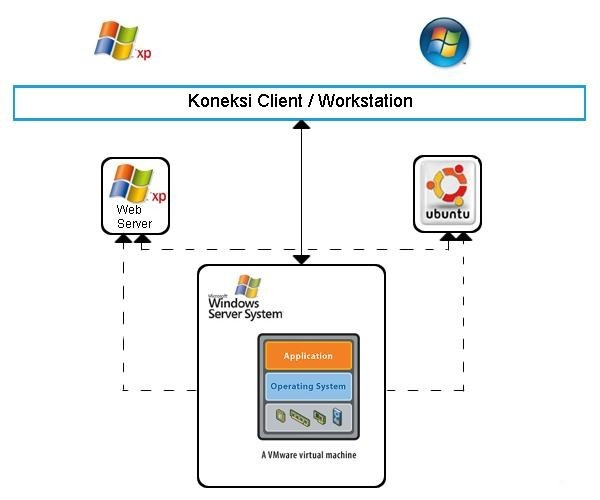
\includegraphics[scale=1]{gambar421.jpg} \\
Gambar 4.2.1 VMware pada Windows Server Enterprise 2003
\end{center}
Topologi jaringan yang terbentuk secara global, seperti yang terlihat pada gambar 4.2.2
\begin{center}
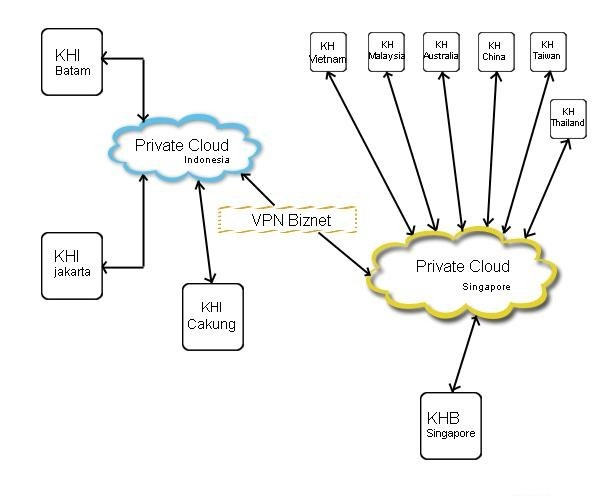
\includegraphics[scale=0.71]{gambar422.jpg} \\
Gambar 4.2.2 Topologi Jaringan Global
\end{center}
Server blade yang menjadi server utama berpusat di Jakarta dan menjadi data center bagi operasional KHI ( Kian Ho Indonesia ). Sedangkan aplikasi penunjang berada dalam mesin virtual, seperti yang terlihat pada gambar 4.2.3
\begin{center}
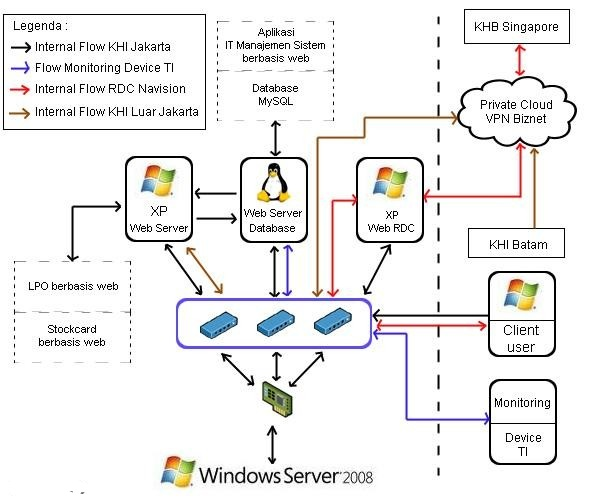
\includegraphics[scale=0.71]{gambar423.jpg} \\
Gambar 4.2.3 Aplikasi Penunjang dalam VM
\end{center}
Windows Server 2008 diimplementasikan ke server blade, dan terbagi dalam tiga mesin virtual yaitu dua buah mesin virtual dengan sistem operasi windows XP, dan satu buah mesin virtual berbasis linux.\\
\tab KHI ( PT Kian Ho Indonesia ) sebagai subsidiary KHB ( Kian Ho Bearing Pte Ltd ) Singapore memiliki autorisasi untuk menerapkan TI policy ( aturan ) secara mandiri untuk diterapkan dalaminfrastruktur  TI di Indonesia.\\
Infrastruktur TI di KHB Singapore menerapkan SCMNavision untuk menunjang operasionalnya, sesuai policy ( aturan ) TI KHB Singapore, semua subsidiary dari KHB diwajibkan untuk menggunakan SCM Navision melalui protocol RDC ( remote desktop connection ) dan koneksi yang terjadi harus melalui VPN internet dengan enkripsi IPSec.\\
Semua pemesanan dan pengiriman barang baik dari Singapore ke Indonesia maupun dari Indonesia ke Singapore melalui software atau aplikasi SCMNavision.\\
\tab Manajemen KHI menyadari pentingnya SCM Navision dalam menunjang  operasional serta menyadari kepentingan internal KHI yang bersifat confidential ( rahasia untuk  KHB  ), maka TI manajemen KHI menyerahkan tanggung jawab koneksi internet ( VPN dan implementasi keamanan transaksi ) kepada provider ISP yaitu  Biznet.\\
Untuk kepentingan internal KHI maka dibuat dua mesin virtual dengan sistem operasi yang sejenis yaitu windows XP ( gambar 4.2.3 ). Mesin virtual pertama menangani dan bertanggung jawab   terhadap   semua   aktifitas  user   ketika  mengakses   web  service,   Pada  mesin  virtual pertama hanya aplikasi yang diimplementasi, tetapi database terkoneksi pada mesin virtual berbasis linux. Aliran alur jaringan dapat dilihat pada gambar 4.2.3 dengan anak  panah berwarna hitam($\rightarrow$).\\
Aplikasi yang diimplementasikan pada mesin virtual pertama adalah LPO berbasis web, dan stockcard berbasis web. Dalam perencanaan TI di kemudian hari skalabilitas dari aplikasi LPO dan stockcard akan ditingkatkan dimana saat ini skalabilitasnya terkoneksi ke BB dan ke email.\\
Aplikasi pada mesin virtual pertama, menggunakan php berbasis framework dengan web servernya adalah Abyss Web Server.
Ketika user dari KHI batam dan KHI cakung terkoneksi ke aplikasi LPO dan stockcard melalui internet, maka server blade yang memiliki IP public dengan kemampuan virtual manajemen sistem vmware, akan menjalankan dan meneruskan request ini ke mesin  virtual  pertama dimana aplikasi LPO dan stockcard diimplementasikan. Aliran alur jaringan dapat dilihat pada gambar 4.2.3 dengan anak panah berwarna coklat (\textcolor{brown}{$\rightarrow$}).\\
/tab Mesin virtual kedua menjadi pusat data dari semua aplikasi internal KHI, database yang digunakan adalah mysql. Aplikasi IT manajemen sistem berfungsi sebagai aplikasi  realtime  yang  memonitor semua device atau peralatan TI yang dijadikan sebagai asset IT.\\
Secara berkala aplikasi IT manajemen sistem akan mengecek kondisi dan status peralatan TI KHI yang berbasis network, hal ini dilakukan dengan tujuan pengendalian atau kontroling terhadap peralatan tersebut, sehingga setiap problem dari peralatan  TI  KHI  dapat  terdeteksi dan mendapatkan alert sistemkepada teamhelpdesk TI KHI. Seperti  yang terlihat pada gambar 4.2.3 dengan anak panah berwarna biru (\textcolor{blue}{$\rightarrow$}).\\
/tab Mesin virtual ketiga merupakan windows XP yang difungsikan sebagai workstation atau komputer client dengan tujuan untuk menyatukan koneksi VPN, dan melakukan remote desktop connection ( RDC ) untuk pemakaian SCM Navision di private cloudnya LHB Singapore
\begin{center}
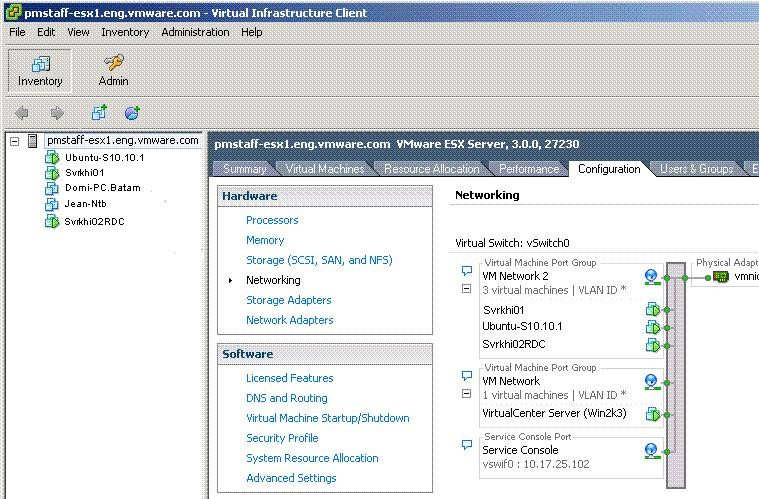
\includegraphics[scale=0.71]{gambar424.jpg} \\
Gambar 4.2.4 interface virtual management  system VMware
\end{center}
\begin{center}
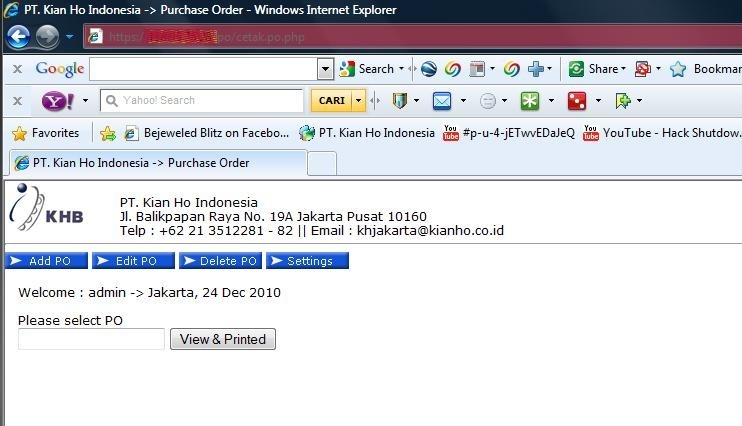
\includegraphics[scale=0.71]{gambar425.jpg} \\
Gambar 4.2.5 aplikasi LPO berbasis web
\end{center}
Gambar 4.2.5 merupakan aplikasi LPO berbasis web yang dapat diakses melalui internet dan untuk keperluan internal. Pengguna memerlukan userid dan password yang setiap bulan akan berganti. Aplikasi ini juga memiliki alert sistem untuk menyetujui transaksi yang terjadi, dan alert tersebut terkirim ke blackberry dan email sistem
\begin{center}
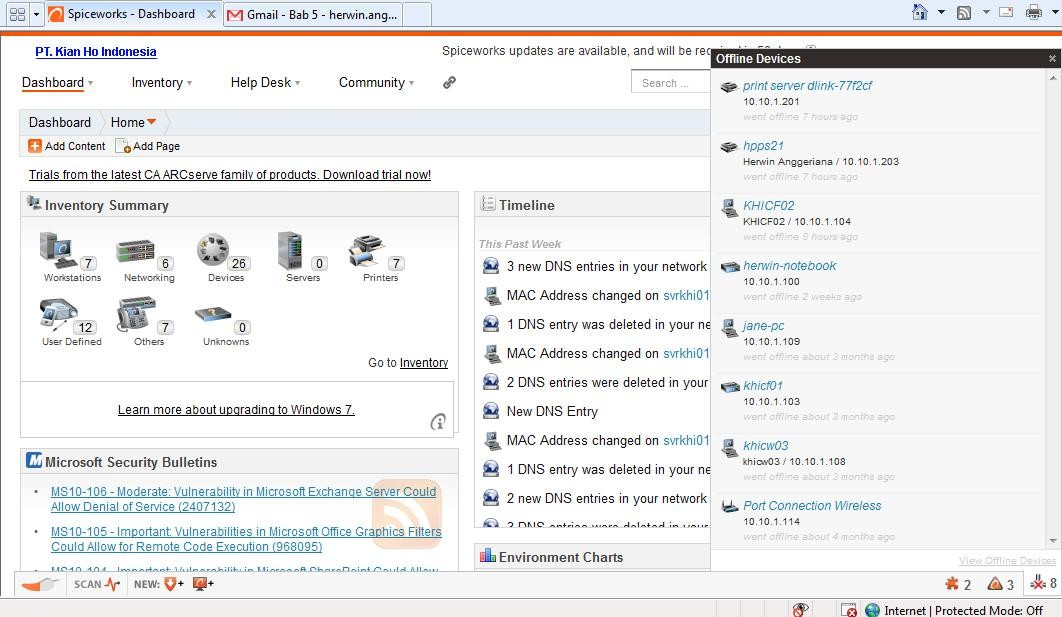
\includegraphics[scale=0.5]{gambar426.jpg} \\
Gambar 4.2.6 aplikasi IT management.
\end{center}
Gambar 4.2.6 merupakan aplikasi IT management system, yang merupakan aplikasi berbasis web dapat diakses melalui internet, dibangun dengan framework php. API yang diterapkan dalamaplikasi ini lebih difokuskan kepada fungsi  monitoring peralatan TI di KHI.
\begin{center}
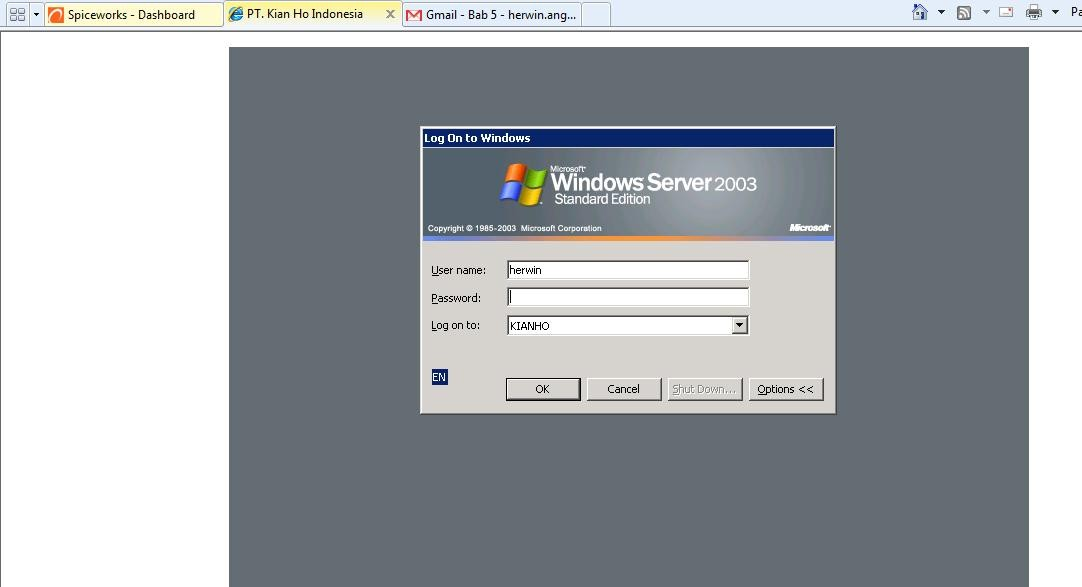
\includegraphics[scale=0.5]{gambar427.jpg} \\
Gambar 4.2.7 remote desktop connection berbasis web.
\end{center}
Gambar 4.2.7 merupakan remote desktop connection berbasis web, diimplementasikan dalam mesin virtual ketiga dengan sistem operasinya windows XP, ketika user  mengakses  mesin virtual ketiga melalui koneksi internet, maka secara automatis mesin virtual ketiga  akan terkoneksi dengan server KHB Singapore.  Aplikasi ini juga menggunakan platform API.\\
Jaringan pada mesin virtual ketiga ini didukung dengan private cloud melalui koneksi internet berbasis VPN IPSec yang disupply oleh provider Biznet.
\begin{center}
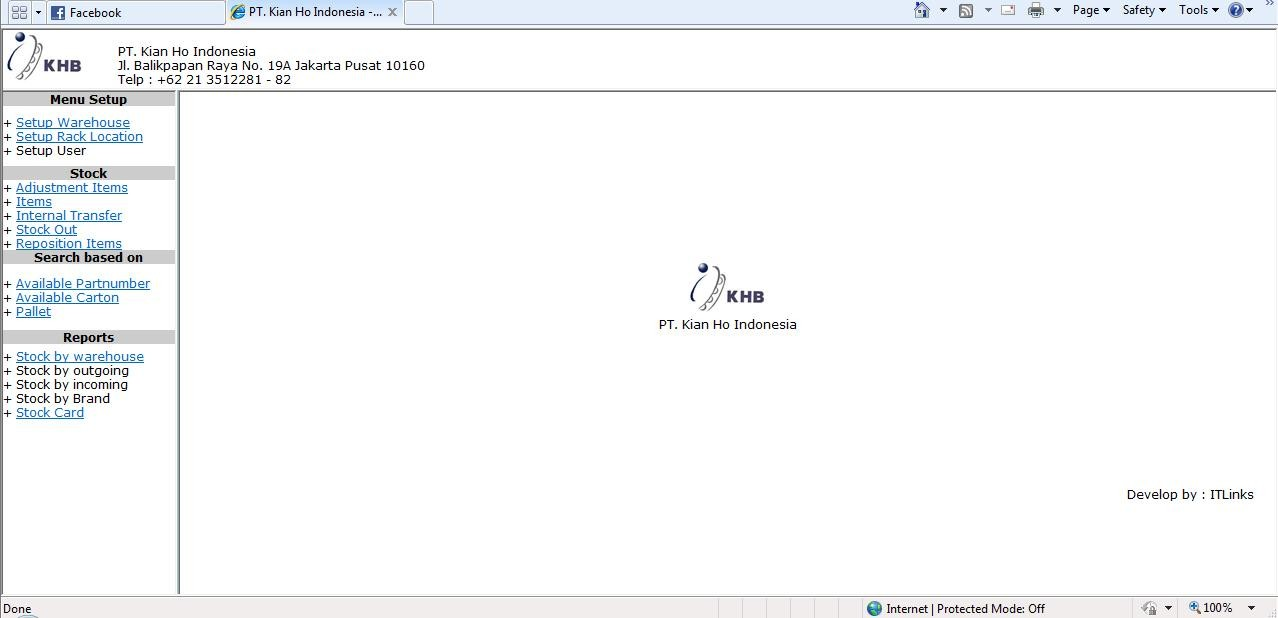
\includegraphics[scale=0.5]{gambar428.jpg} \\
Gambar 4.2.8 aplikasi stockcard berbasis web.
\end{center}
Gambar 4.2.8 merupakan aplikasi stockcard berbasis web yang  diimplementasikan  dalam  mesin virtual pertama, dengan database yang berada di mesin virtual kedua dengan sistem operasi linux.
\let\cleardoublepage\clearpage
\begin{thebibliography}{99}
\bibitem{BarnettAlex} 
Barnett, Alex. So what is this Platformas a Service Thing
\\\texttt{http://alexbarnett.net}

\bibitem{Llorente} 
Llorente, I. M. 
\textit{Towards a new model for the infrastructure grid. Panel FromGrids to Cloud Services in the International Advanced Research Workshop on High Performance Computing and Grids}. Cetraro, Italy, July 2008.
 
\bibitem{Andressen} 
Andressen, Marc. The three kinds of platforms you meet on the Internet
\\\texttt{http://blog.pmarca.com}

\bibitem{MacVittie} 
MacVittie, Lori. As a Service: The many faces of the cloud
\\\texttt{http://devcentral.f5.com/weblogs/macvittie/Default.aspx}

\bibitem{Macvitti} 
MacVittie, Lori. Bursting the Cloud
\\\texttt{http://devcentral.f5.com/weblogs/macvittie/archive/2008/09/03/}

\bibitem{Webopedia} 
Webopedia Computer Dictionary. data center tiers 
\\\texttt{http://www.webopedia.com/TERM/D/data\_center\_tiers.html}

\bibitem{Andreessen} 
Andreessen, Marc. Analyzing the Facebook Platform
\\\texttt{http://blog.pmarca.com/2007/06/analyzing\_the\_f.html}

\bibitem{Meredith} 
Farkas, Meredith. What is Social Software?
\\\texttt{http://www.sociallibraries.com/farkaschap1.pdf}

\bibitem{Takase} 
Takase, Akihiko D. Sc. And Kikuchi, Susumu. Platform Architecture for Networked Businesses
\\\texttt{http://hitachi.com/ICSFiles/afieldfile/2004/06/01/r2000\_04\_101.pdf} 
 
\bibitem{Webopedia} 
Webopedia Computer Dictionary. data center tiers
\\\texttt{http://www.webopedia.com/TERM/D/data\_center\_tiers.html}

\bibitem{Andrei} 
Andrei Hagiu and David B. Yoffie. Business Harvard Review 
\\\texttt{http://www.hbr.org}

\bibitem{Webopedia} 
Jerry Shenk. Log Management in the Cloud
\\\texttt{http://www.sans.org/}
\end{thebibliography}
\let\cleardoublepage\clearpage
\end{document}
